\documentclass[10pt,a4paper,master=cws, masteroption=ai,english,inputenc=utf8]{kulemt}
\setup{title={Secure Compilation of ML Modules},
       author={Matthias van der Hallen},
       promotor={Prof. dr. ir. F. Piessens},
       assessor={Dr. ir. W. Meert \and Dr. D. Devriese},
       assistant={M. Patrignani \and R. Strackx}}
\setup{filingcard, translatedtitle={Veilige Compilatie van ML-stijl Modulesystemen},
        udc=621.1,
        shortabstract={Malware infects many new computers each day.
Some estimates suggest that up to 30\% of all computers are in fact infected.
This malware is transmitted by exploiting bugs in computer software.
In many cases, these bugs abused by the exploit originate from the disparity between the computing model presented by high-level source language and the effective module used by the low-level target language.
\\
These bugs are not prevented by analysis of the source language, for example using formal software verification tools, because they are effectively `introduced' by the process of compilation from source language to target language.
Instead, they must be prevented by strengthening the compilation process in a way that reduces the power of low-level attackers to that of high-level attackers.
Compilers that achieve this provide `secure compilation'.
\\
This work uses the notions of full abstraction and contextual equivalence to formalize the requirements for a secure compilation scheme, and shows how secure compilation can be achieved for MiniML, a subset of the ML language.
As a prerequisite however, the secure compilation scheme assumes that the result of compilation runs on an architecture that provides program counter based access control, called a protected module platform.
\\
The source language for this secure compilation scheme, MiniML, is not object oriented. 
Instead it uses a module system with the powerful notion of a functor to provide modularization of code.
It targets the LLVM Intermediate Representation as a target language.
A formalization of this MiniML source language and the LLVM IR target language is presented, enabling a formalization of the secure compilation scheme to be given as well.}}
%\usepackage[utf8]{inputenc}
\usepackage{amsmath}
\usepackage{amsfonts}
\usepackage{amssymb}
\usepackage{todonotes}
\usepackage{hyperref}
\usepackage{listings}
\usepackage{float}
\usepackage{lmodern}
\usepackage{graphicx}
\usepackage{caption}
\usepackage{subcaption}
\usepackage{xcolor,colortbl}
%\usepackage{longtable}
\usepackage{ltablex}
\usepackage{appendix}
\usepackage{amsthm}
%\usepackage{tabu}
%\usepackage{longtabu}
%\usepackage[sorting=none, style=authoryear, backend=bibtex]{biblatex}
%\addbibresource{bibliography.bib}
%\usepackage[style=mla,babel=hyphen,backend=biber]{biblatex}
%\usepackage[square]{natbib}
%\setcitestyle{authoryear,square}
%\usepackage{courier}

%\setlength\parindent{1em}


\lstset{basicstyle=\ttfamily,breaklines=true, keepspaces=true, columns=flexible, numberstyle=\small,escapeinside={±}{±}}
%\lstset{language=ML}
\lstset{
 morekeywords={where}
}
\renewcommand{\lstlistlistingname}{List of Listings}
\newcounter{line}


\DeclareMathOperator\compat{\ensuremath{\raisebox{1mm}{$\frown$}}}
\DeclareMathOperator\nsimeq{\ensuremath{\simeq\!\!\!\!\!/\ }}
\DeclareMathOperator\rbisim{\ensuremath{\mc{R}}} 
\DeclareMathOperator\impl{\ensuremath{\Rightarrow}} 
\DeclareMathOperator\teq{\ensuremath{\simeq_{T}}}
\DeclareMathOperator\nteq{\ensuremath{\nsimeq\!\!_{T}}}
\DeclareMathOperator\oeq{\ensuremath{\simeq_{O}}}
\DeclareMathOperator\wbis{\ensuremath{\approx}}

%%%%%%%%%%%%%%%%%%%%% fonts
\newcommand{\mt}[1]{\ensuremath{\texttt{#1}}}
\newcommand{\mtt}[1]{\ensuremath{\mathtt{#1}}}
\newcommand{\mf}[1]{\ensuremath{\mathbf{#1}}}
\newcommand{\mi}[1]{\ensuremath{\mathit{#1}}}
\newcommand{\mc}[1]{\ensuremath{\mathcal{#1}}}
\newcommand{\ms}[1]{\ensuremath{\mathsf{#1}}}
\newcommand{\mb}[1]{\ensuremath{\mathbb{#1}}}

%%%%%%%%%%%%%%%%%%%%% shorts
\newcommand{\acron}[0]{\ensuremath{\mbox{FPMAC}}\xspace}
\newcommand{\acrons}[0]{\ensuremath{\mbox{FPMACs}}\xspace}

\newcommand{\OB}[1]{\ensuremath{\overline{#1}}}
\newcommand{\subt}[0]{\ensuremath{<:}}
\newcommand{\xto}[1]{\ensuremath{\xrightarrow{~#1~}}}
\newcommand{\Xto}[1]{\ensuremath{\xRightarrow{~#1~}}}
\newcommand{\xtol}[1]{\ensuremath{\xrightarrow{~#1~}\low}}
\newcommand{\Xtol}[1]{\ensuremath{\xRightarrow{~#1~}\Low}}
\newcommand{\nXtol}[1]{\ensuremath{\xRightarrow{~#1~}\nLow}}
\newcommand{\tol}[0]{\ensuremath{\to}} %{\to\low}}
\newcommand{\low}[0]{\ensuremath{\!\!\!\!\to} }
\newcommand{\Low}[0]{\ensuremath{\!\!\!\!\Rightarrow} }
\newcommand{\nLow}[0]{\ensuremath{\!\!\!\!\!\!\!\!/\!\!\Rightarrow} }
\newcommand{\da}[0]{\ensuremath{^{\downarrow}}}
\newcommand{\ua}[1]{\ensuremath{\uparrow\!\!(#1)}}
\newcommand{\Ua}[0]{\ensuremath{\Uparrow}}
\newcommand{\myset}[2]{\ensuremath{\{#1 ~|~ #2\}}}
\newcommand{\sta}[1]{\ensuremath{\widehat{#1}}}

\newcommand{\toli}[0]{\ensuremath{\to^{\!\!\!\!\!i}\ }}
\newcommand{\tole}[0]{\ensuremath{\to^{\!\!\!\!\!e}\ }}


\newcommand{\jjr}[0]{Java~Jr.\xspace}

\newcommand{\divr}[0]{\ensuremath{\!\!\Uparrow\xspace}}

\newcommand{\totr}[1]{\ensuremath{\lfloor #1 \rfloor}}
\newcommand{\toex}[1]{\ensuremath{\lceil #1 \rceil}}

\newcommand{\fun}[2]{\ensuremath{\mtt{#1}(#2)}}
\newcommand{\dom}[1]{\ensuremath{\fun{dom}{#1}}}
\newcommand{\mex}[1]{\ensuremath{\fun{m_{ext}}{#1}}}
\newcommand{\mse}[1]{\ensuremath{\fun{m_{sec}}{#1}}}
\newcommand{\stu}[0]{\ensuremath{^{\bot}\xspace}}
\newcommand{\ldiv}[0]{\ensuremath{^{\Uparrow L}\xspace}}

\newcommand{\assline}[1]{\arabic{line}~~ \mtt{#1}\stepcounter{line}}

\newcommand{\sps}[0]{\ms{SP_{sec}}\xspace}
\newcommand{\spe}[0]{\ms{SP_{ext}}\xspace}

\newcommand{\TL}[1]{\ensuremath{\ms{Tr}(#1)}}
\newcommand{\trl}[0]{\ensuremath{\ms{Tr^L}}\xspace}
\newcommand{\trs}[0]{\ensuremath{\ms{Tr^S}}\xspace}

\newcommand{\blk}[0]{\ensuremath{(\ms{unknown},m,s)}\xspace}

\newcommand{\comm}[1]{}
%%%%%%%%%%%%%%%%%%%%%%%% typing & rules 
\newcommand{\typerule}[3]{\ensuremath{\begin{array}{c}\textsf{\scriptsize ({#1})} \\#2 \\\hline\raisebox{-3pt}{\ensuremath{#3}}\end{array}}}

\newcommand{\raisedrule}[2][0em]{\leaders\hbox{\rule[#1]{1pt}{#2}}\hfill}

\newcommand{\toprule}[1]{\begin{center}\vspace{1mm}\noindent\raisedrule{0.3mm}\ \raisebox{-0.5ex}{\emph{#1}} \raisedrule{0.3mm}\!\raisedrule{0.3mm}\!\raisedrule{0.3mm}}

\newcommand{\botrule}{\vspace*{2mm}\HRule\end{center}}

\newcommand{\HRule}[0]{\rule{\linewidth}{0.3mm}\vspace*{-1mm}}%\rule{\linewidth}{0.3mm}}

%%%%%%%%%%%%%%%%%%%%%%%% misc
\newcommand{\MP}[1]{\todo[color=blue!30]{TODO:#1}}
\newcommand{\myparagraph}[1]{\smallskip \noindent\noindent\textit{#1.}~~}


%%%%%%%%%%%%%%%%%%%%%%%% environments
\newtheorem{assumption}{Assumption}
\newtheorem{notation}{Notation}


\newenvironment{proofsketch}{\trivlist\item[]\emph{Proof Sketch}.\xspace}{\unskip\nobreak\hskip 1em plus 1fil\nobreak$\Box$\parfillskip=0pt\endtrivlist}


%%%%%%%%%%%%%%%%%%%%%%%% pictures
\pgfdeclarelayer{background}
\pgfdeclarelayer{back2}
\pgfdeclarelayer{foreground}
\pgfsetlayers{background,back2,main,foreground}

\newcommand{\tikzpic}[1]{
\begin{tikzpicture}[shorten >=1pt,auto,node distance=6mm,rounded corners]
\tikzstyle{state} =[fill=white,minimum size=4pt]
#1
\end{tikzpicture}
}
\newcommand{\myfig}[3]{\begin{figure} [!h]
#1
\caption{\label{fig:#2}#3}
\end{figure}}

\newcommand{\myfigb}[3]{\begin{figure} [!b]
#1
\caption{\label{fig:#2}#3}
\end{figure}}

%%%%%%%%%%%%%    Easier way to use references   
\newcommand{\customref}[2]{\hyperref[#2]{#1~\ref*{#2}}}

\newcommand{\myref}[2]{%
  \ifthenelse{\equal{#1}{lst}}{\customref{Listing}{#2}}{
  \ifthenelse{\equal{#1}{fig}}{\customref{Fig.}{#1:#2}}{%
  \ifthenelse{\equal{#1}{def}}{\customref{Definition}{#1:#2}}{%
  \ifthenelse{\equal{#1}{lem}}{\customref{Lemma}{#1:#2}}{%
  \ifthenelse{\equal{#1}{thm}}{\customref{Theorem}{#1:#2}}{%
  \ifthenelse{\equal{#1}{not}}{\customref{Notation}{#1:#2}}{%
  \ifthenelse{\equal{#1}{prop}}{\customref{Proposition}{#1:#2}}{%
  \ifthenelse{\equal{#1}{ax}}{\customref{Axiom}{#1:#2}}{%
  \ifthenelse{\equal{#1}{ex}}{\customref{Example}{#1:#2}}{%
  \ifthenelse{\equal{#1}{propr}}{\customref{Property}{#1:#2}}{%
  \ifthenelse{\equal{#1}{ass}}{\customref{Assumption}{#1:#2}}{%
  \ifthenelse{\equal{#1}{tab}}{\customref{Table}{#1:#2}}{%
  \ifthenelse{\equal{#1}{sec}}{\hyperref[#2]{Section~\ref*{#2}}}{%
  \ifthenelse{\equal{#1}{eq}}{\hyperref[#1:#2]{Equation~(\ref*{#1:#2})}}{%
    \ifthenelse{\equal{#1}{for}}{\hyperref[#1:#2]{Formula~(\ref*{#1:#2})}}{%
  \autoref{#1:#2}%
  }}}}}}}}}}}}}}}}
  
  
%use only when citing Example 1 and 2.  The Example 1 is cited with \myref, in order to obtain the right 2, use \myrefdrop
\newcommand{\myrefand}[2]{%
  \ifthenelse{\equal{#1}{fig}}{\customref{}{#1:#2}}{%
  \ifthenelse{\equal{#1}{def}}{\customref{}{#1:#2}}{%
  \ifthenelse{\equal{#1}{lem}}{\customref{}{#1:#2}}{%
  \ifthenelse{\equal{#1}{not}}{\customref{}{#1:#2}}{%
  \ifthenelse{\equal{#1}{thm}}{\customref{}{#1:#2}}{%
  \ifthenelse{\equal{#1}{prop}}{\customref{}{#1:#2}}{%
  \ifthenelse{\equal{#1}{ax}}{\customref{}{#1:#2}}{%
  \ifthenelse{\equal{#1}{ex}}{\customref{}{#1:#2}}{%
  \ifthenelse{\equal{#1}{propr}}{\customref{}{#1:#2}}{%
  \ifthenelse{\equal{#1}{ass}}{\customref{}{#1:#2}}{%
  \ifthenelse{\equal{#1}{tab}}{\customref{}{#1:#2}}{%
    \ifthenelse{\equal{#1}{lis}}{\customref{}{#1:#2}}{%
  \ifthenelse{\equal{#1}{sec}}{\hyperref[#1:#2]{\ref*{#1:#2}}}{%
  \ifthenelse{\equal{#1}{eq}}{\hyperref[#1:#2]{(\ref*{#1:#2})}}{%
    \ifthenelse{\equal{#1}{for}}{\hyperref[#1:#2]{(\ref*{#1:#2})}}{%
  \autoref{#1:#2}%
  }}}}}}}}}}}}}}}}
  
\newcommand{\etal}[0]{\textit{et al.}\xspace} 



%%%%%%%%%%%%%%%%%%%%%%listing options
\lstdefinelanguage{Java} %thanks to whoever did this
{morekeywords={abstract, all, and, as, assert, but, check, disj, else, exactly, extends, fact, for, fun, iden, if, iff, implies, in, Int, int, let, lone, module, no, none, not, one, open, or, part, pred, run, seq, set, sig, some, sum, then, univ, package, class, public, private, null, return, new, interface, extern, object, implements, System, static},
sensitive=true,morecomment=[l][\small\itshape]{--},morecomment=[l][\small\itshape]{//},morecomment=[s][\small\itshape]{/*}{*/},basicstyle=\small,
%basicstyle=\ttfamily,
numbers=left,numberstyle=\scriptsize,tabsize=2,numbersep=3pt,breaklines=true,lineskip=-2pt,stepnumber=1,captionpos=b,breaklines=true,breakatwhitespace=false,showspaces=false,showtabs=false,
%frame=single,
columns=fullflexible,escapeinside={(*@}{@*)},
literate={->}{{$\to$}}1 {^}{{$\mspace{-3mu}\widehat{\quad}\mspace{-3mu}$}}1
{<}{$<$ }2 {>}{$>$ }2 {>=}{$\geq$ }2 {=<}{$\leq$ }2
{<:}{{$<\mspace{-3mu}:$}}2 {:>}{{$:\mspace{-3mu}>$}}2
{=>}{{$\Rightarrow$ }}2 {+}{$+$ }2 {++}{{$+\mspace{-8mu}+$ }}2
{<=>}{{$\Leftrightarrow$ }}2 {+}{$+$ }2 {++}{{$+\mspace{-8mu}+$ }}2
{\~}{{$\mspace{-3mu}\widetilde{\quad}\mspace{-3mu}$}}1
{!=}{$\neq$ }2 {*}{${}^{\ast}$}1 %{.}{$\cdot$}1
{\#}{$\#$}1
}
\lstset{language=Java,numbersep=5pt,frame=single}

%\bibliography{bibliography}

\begin{document}
%\newcommand{\emphref}[1]{\emph{}}
\newcommand{\MiniML}{\mbox{MiniML}} %The stylish representation of MiniML
\newcommand{\cmath}[1]{\ensuremath{\mathit{#1}}} %correct Math text
\newcommand{\lsttext}[1]{\lstinline[mathescape]!#1!} %inline text as in listings
\newcommand{\longspace}{\;\;\;\;\;\;}
\newcommand{\inlinecode}{\texttt}
\newcommand{\expl}[1]{{\text{\footnotesize#1}}}
\newcommand{\LLVMIR}{\mbox{LLVM IR}}
%\newcommand{\compile}[1]{\mathit{\left[\left[#1\right]\right]}}
\newcommand{\compiled}[1]{#1^{\downarrow}}
%\newcommand{\makes}{& \rightarrow}
\newcommand{\ova}{\overline{\alpha}}
\newcommand{\gray}{\cellcolor{lightgray}}
\newcommand{\earlier}[2]{{\protect\myref{#1}{#2}} on {\protect\mypageref{#2}}}
\newcommand{\intertextt}[1]{
& & \\
\multicolumn{3}{@{}p{\textwidth}@{}}{\indent#1}\\
& & \\
}
\newcommand{\annot}[1]{[#1]}
\newcommand{\nl}{\\ & &}
\newcommand{\makes}{& \ensuremath{\rightarrow} &}
\newcommand{\compile}[1]{[[#1]]}
\newcommand{\mypageref}[1]{Page~\pageref{#1}}

%Describe an attack nicely.
\newcommand{\surroundrule}[2][0.3em]{
\leavevmode\raisedrule[#1]{1pt}#2\raisedrule[#1]{1pt}}
\newenvironment{attack}[1]{\par\par\noindent\hspace{-1ex}\surroundrule{#1}\vspace{-0.5em}\par\par}{~\vspace{0.5em}\par\par\noindent\leavevmode\raisedrule[1em]{1pt}\\}
%\begin{flushleft}


\hypersetup{colorlinks=false, pdfborder={0 0 0}}

\begin{preface}
I would like to thank everyone who helped me to produce this master thesis.
First, I would like to thank my promoter,
prof. dr. ir. Frank Piessens, for providing me with this opportunity.
Next, many thanks go out to my supervisors, M. Patrignani and R. Strackx for supporting me throughout the year.
Futhermore, I would like to thank my friends and classmates with whom many moments of joy or frustration could be shared.
Finally, I would like to thank my family for the encouragement and moral support I was lucky to receive.
\end{preface}

\tableofcontents*
\listoffigures
\lstlistoflistings

\begin{abstract}
Malware infects many new computers each day.
Some estimates suggest that up to 30\% of all computers are in fact infected.
This malware is transmitted by exploiting bugs in computer software.
In many cases, these bugs abused by the exploit originate from the disparity between the computing model presented by high-level source language and the effective module used by the low-level target language.

These bugs are not prevented by analysis of the source language, for example using formal software verification tools, because they are effectively `introduced' by the process of compilation from source language to target language.
Instead, they must be prevented by strengthening the compilation process in a way that reduces the power of low-level attackers to that of high-level attackers.
Compilers that achieve this provide `secure compilation'.

This work uses the notions of full abstraction and contextual equivalence to formalize the requirements for a secure compilation scheme, and shows how secure compilation can be achieved for MiniML, a subset of the ML language.
As a prerequisite however, the secure compilation scheme assumes that the result of compilation runs on an architecture that provides program counter based access control, called a protected module platform.

The source language for this secure compilation scheme, MiniML, is not object oriented. 
Instead it uses a module system with the powerful notion of a functor to provide modularization of code.
It targets the LLVM Intermediate Representation as a target language.
A formalization of this MiniML source language and the LLVM IR target language is presented, enabling a formalization of the secure compilation scheme to be given as well.
\end{abstract}

%\begin{abstract*}
%\end{abstract*}


\mainmatter
\chapter{Introduction}

In today's technology-driven world, computer software is used by nearly everyone on a daily basis.
The near omnipresence of malware trying to infect computers makes \emph{safety} a continuous concern for anyone involved in the creation of this computer software.
Partly, this can be done by verifying that no bugs exist in the source code of the software, for example using verification software~\cite{Verifast:paper,Verifast:tutorial}.

However, a formal verification of the source code can only show that no source-level bugs exist.
After a program's source code has been written, it is usually compiled to a target language such as assembly that can be executed.
This target language most often is substantially different from the source language.
These differences are a direct consequence of the simplified computing model that high-level languages usually offer to the programmer.
For example, high-level languages often hide the fact that values have to be represented using target-language concepts, saved in computer memory.
The compilation process reintroduces these concerns.

In many instances, malware exploits target-level bugs introduced by this compilation process~\cite{OVSPaper,Younan:2012:RCC:2187671.2187679}.
These bugs do not show up during formal verification of the source code, as they are only introduced when the abstract computing model used on source-level is traded in for the concrete target-level computing model.

To provide security, the compilation process itself must be strengthened, so that it guarantees that any source-level security guarantees are preserved throughout the compilation step from source language to target language.
If this is achieved, then any software that is attack-free on the source-level is attack-free as well on the target-level.
A compilation scheme able to provide these guarantees is rightly called secure.
Effectively, such a compilation scheme reduces the capabilities of a target-level attack to those of a source-level attack.
The aim of this thesis is to describe how secure compilation can be achieved for a \emph{functional} language that implements an \emph{ML-style} module system.

%This is formalized using the \emph{full abstraction}~\cite{Abadi} concept.

\section{Secure Compilation}
\label{sec:SecureCompilation}
Software programs or libraries are usually written in a source language, to be followed by compilation to a target language.
Often, the main reason for this distinction is that it is easier to reason about the program in the source language than at the target language.
This is because the source language works at a higher level of abstraction than the target language.

For example, a high-level source language such as Java abstracts away all concerns a programmer might have about how to handle computer memory.
The representation of an object defined by the programmer in memory, as well as the location of this object is all hidden away.
Effectively, the source language takes the burden of handling these daunting tasks away from the programmer.

This is a form of \emph{data abstraction}: objects are described by their properties and the functionality they offer, not by their implementations.
Here data abstraction concerns hiding the implementation of basic types by bits in memory, but most high-level languages offer the same software principle by allowing abstract data types. 
An abstract data type is implemented using basic types offered by the source language, but whenever a value of this type is used, only its described properties and abstract functionality are available.

Data abstraction is part of an abstraction paradigm provided by a source language, called \emph{information hiding}.
Information hiding happens any time that some value, function or datatype is implemented, but its use is restricted: it is hidden.

Another abstraction paradigm that the source language can provide is called \emph{modularization}.
Modularization offers a way to group closely related functionality together. For example, in Java this would correspond to a class or a group of classes, called a package.

Modularization and information hiding are closely related and affect each other to allow for \emph{encapsulation}, where the internal representation is hidden so that it influences only a small, identifiable region of the program~\cite{Pierce}.
The information hiding mechanisms of Java for example, the \lstinline[language=Java]{private, public, protected} and \lstinline[language=Java]{default} access modifiers, differ from one another in how they handle the different modularization mechanisms: classes and packages.
Public functionality can be used everywhere, private functionality only within the same class, whereas the default access modifier allows access from any class within the same package.
\\[1em]
These abstractions not only make it easier for the programmer to reason about the correctness of software, they also provide a way to describe security properties.
When a value or function is marked with an access modifier, any programmer rightly assumes these access rights are indeed enforced.
A value marked \lstinline[language=Java]{private} can only be read of modified by certain parts of the code.
In security terms these access modifiers provide \emph{confidentiality} and \emph{integrity}.
Even formal verification tools to keep the software free from bugs assume the enforcements of these access rights.

The target language, however, does not always offer these abstractions.
For example, when executing software, the values created by this software must be saved in memory, using a certain representation.
The platform on which the target language runs might not provide access control for this memory, which means values saved in memory might be readable by any code running on the platform.

Software code must be saved somewhere as well, and doing this might corrupt control flow, for example by overwriting a return address~\cite{OVSPaper}.
Such an attack might result executing functionality that was supposed to be hidden.

\subsubsection{Full Abstraction}
\label{sec:fullabstraction}
Secure compilation is a compilation process that does preserve these source-level security properties when compiling to the target language.
In this work, this property of a compiler is formalized as \emph{full abstraction}~\cite{Abadi}.
Full abstraction uses the idea of \emph{contextual equivalence} to formalize security guarantees.

Contextual equivalence is an equivalence relation on programs.
The contextual equivalence relation $O_{1} \simeq O_{2}$ expresses that two programs $O_1$ and $O_2$ are indistinguishable from each other, even when running them in combination with any other program $O_C$ called the context.
Informally, this corresponds with there being no \emph{observable} differences between $O_1$ and $O_2$.
Formally, $O_{1} \simeq O_{2}$ means:

\[
    \forall O_C : O_C[O_{1}] \rightarrow c \iff O_C[O_{2}] \rightarrow c
\]
where $O_{C}[.]$ is a program where a certain component is missing. 
$O_{C}[O_1]$ is the program that results from linking $O_C$ with $O_1$, where $O_1$ is used as the missing component.

Note that contextual equivalence does indeed imply security guarantees are enforced.
Suppose that two programs $O_1$ and $O_2$ differ only by a value that is supposedly confidential.
If it were possible for any context to read or modify this value, then this context provides a counter example for the statement that two programs that use a different hidden value are contextually equivalent.
%Breaking a security guarantee means disproving contextual equivalence.
\\[1em]
As contextual equivalence implies that security guarantees are enforced, secure compilation can be formalized as providing \emph{full abstraction}, meaning contextual equivalence is preserved and reflected when compiling a program $O_1$ to its corresponding target language program $\compiled{O_1}$. 
Formally:

\[
    O_{1} \simeq O_{2} \iff \compiled{O_{1}} \simeq \compiled{O_{2}}
\]

In the remainder of this text, the program $O_1$ or $O_2$ presents the secure code, an encapsulated entity for which some security guarantees hold.
The secure compilation of this encapsulated entity is called the self-protected module or \emph{SPM}.
The secure code is provided and compiled to an \emph{SPM}, and is linked to an insecure target level context $\compiled{O_C}$

\section{Protected Module Architecture}
\label{sec:protectedmodulearchitecture}
As explained in \myref{sec}{sec:SecureCompilation}, a secure compilation scheme is a compilation scheme that preserves source level security guarantees in the target language.
Such a preservation of security guarantees is only possible if some form of access controlled memory is available.

Indeed, if no protection of any memory where possible, no confidentiality could ever be preserved, as values would always be readable directly from memory.
For this reason, the securely compiled module is to an architecture that provides \emph{program counter based access control}~\cite{PCBAC} or \emph{PCBAC}.
Such an architecture is called a \emph{Protected Module Architecture}. 
The term \emph{program counter based access control} refers to the fact that the validity of a memory access depends on the current location of the program counter.

The semantics of the access control imposed by the platform are given in \myref{fig}{fig:AccessControlSemantics}.
This work uses the same memory access control model as given by Agten et al. in~\cite{Agten:2012:SCM:2354412.2355247}.
As shown by Patrignani et al.~\cite{Patrignani} the same access control model can be used to provide secure compilation for more advanced concepts object oriented programming concepts.

\begin{figure}[htb]
    \centering
	\begin{tabular}{|c|c|c|c|c|}
		\hline
		From \textbackslash To & \multicolumn{3}{c|}{Protected} & Unprotected \\
		& Entry Point & Code & Data & \\ \hline
		Protected & r x & r x & r w & r w x \\ \hline
		Unprotected & x & & & r w x \\ \hline
	\end{tabular}
    \caption[PCBAC Semantics]{Program counter based access control semantics as specified in Agten et al.~\cite{Agten:2012:SCM:2354412.2355247}. \label{fig:AccessControlSemantics}}
\end{figure}

The \emph{SPM} created by secure compilation is loaded in the \emph{protected} memory.
The code associated with an \emph{SPM} is located in the code section of the protected memory, memory allocations are done within the data section of protected memory.
An \emph{SPM} must also provide a list of \emph{entry points}, which are specific positions within the protected code section.
The insecure context is loaded in \emph{unprotected} memory.

The access control mechanism imposes that the insecure context can only divert control flow to entry points or other parts of the unprotected memory.
Its read and write access is also limited to the unprotected memory.
The \emph{SPM} has \emph{read} as well as \emph{execute} permissions for its entire code section, including its entry points.

There are already a few architectures that support these program counter based access control semantics, or a variation of them~\cite{Fides, Salus, Sancus}.

\section{Thesis Structure}
This thesis aims to show how secure compilation can be achieved for a \emph{functional} language that implements an \emph{ML-style} module system.
For this, a source language, \emph{\MiniML}, is defined as a subset of the functionality provided by the ML programming language.

A target language to which \MiniML\ will be compiled has to be chosen as well.
In this thesis, the \emph{LLVM Intermediate Representation} is used.
The LLVM Intermediate Representation is a language used in the LLVM compiler project.
As a language it is only slightly more abstract than assembly, and it is specifically designed as an intermediate step in the compilation of different high-level source languages to assembly.

This offers the benefit that compilation to the intermediate language can be performed, and afterwards transformations can be done on the intermediate language to optimize it for different architectures.
Afterwards, the LLVM Intermediate representation can be compiled to assembly code for a specific architecture, for example an architecture providing the necessary access control sketched in \myref{sec}{sec:protectedmodulearchitecture}.
\\[1em]
The following list gives a roadmap of how each chapter contributes to the thesis goal of showing how secure compilation of a language with an \emph{ML-style} module system is possible.

\begin{itemize}
\item 
\myref{chap}{chap:ACompilationExample} describes a first version of the \MiniML\ language, mimicking some of the basic functionality provided by the ML language and its module system, using an example: An implementations of a Caesar cipher.

It also describes the target-language, \LLVMIR, and shows how compilation from \MiniML\ to LLVM might normally occur.

It concludes by describing the security issues that must be solved and shows how secure compilation would address these using the example.

\item
\myref{chap}{chap:formalspecification} gives a formalization of both the \MiniML\ source language and the \LLVMIR\ target language.
It then formally describes a secure compiler for this first version of \MiniML.

\item
\myref{chap}{chap:AdvancedConcepts} introduces some more advanced ML concepts to \MiniML.
Specifically, \emph{higher order functions} and \emph{functors}.

\item
\myref{chap}{chap:FormalizationOfAdvancedConcepts} extends the formalization of \MiniML\ given in \myref{chap}{chap:formalspecification} to include the advanced concepts that were introduced to \MiniML\ in \myref{chap}{chap:AdvancedConcepts}.

It proceeds by extending the formalization of the secure compiler of \myref{chap}{chap:formalspecification}.

\item
\myref{chap}{chap:InformalProof} details how full abstraction of a compilation scheme can be proven.
%, and gives an informal argument suggesting that the compilation scheme presented in \myref{chap}{chap:FormalizationOfAdvancedConcepts}

\item
\myref{chap}{chap:conclusion} gives an overview of possible improvements or extensions of the work presented here.
It also formulates a conclusion to this thesis.
\end{itemize}

\chapter{A Compilation Example}
\label{chap:ACompilationExample}
This chapter firstly informally describes the \mbox{MiniML} source language (\myref{sec}{sec:MiniML}), a subset of the ML language whose syntax and semantics are reminiscent of those of Standard ML.
\myref{sec}{sec:MLExample} then introduces an example program that will be used to show the secure compilation scheme.
This chapter continues by describing the LLVM intermediate language to which the first translation occurs (\myref{sec}{sec:LLVM}).
This chapter concludes by translating the earlier proposed example program, showing the resulting LLVM code.
%The secure compilation scheme is shown from an example program written in the source language, \mbox{MiniML}, which is a subset of the ML language. Its syntax and semantics are reminiscent of those used in Standard ML.

\section{MiniML}
\label{sec:MiniML}
The ML language is a functional programming language which is well known for its module system.
This module system aims to group data and code together into coherent entities, called the modules.

A \emph{structure} is the most basic type of module.
It can be defined using the \lsttext{struct} construct and provides a set of bindings for types, values and functions.
A structure specifies a name for the binding and the corresponding value, called \emph{implementation}.
Structures provide the possibility of grouping related code and data, fulfilling the need of \emph{encapsulation} in software.
However, the need for \emph{data abstraction} is not yet fulfilled.
\myref{lst}{code:DictionaryStructureExample} shows how a dictionary of strings to strings might be implemented by a module.
~
\begin{lstlisting}[frame=single, language=ML,caption=An example structure showing the definition of a dictionary in ML, label=code:DictionaryStructureExample,numbers=left]
structure Dictionary =
    struct
        type dictionary = (string * string) list
        val emptyDictionary = []
        fun insert d, x, y = (x,y)::d
    end
\end{lstlisting}

\myref{lst}{code:DictionaryStructureExample} firstly defines a type dictionary, which is defined to be a type synonym for a list of string pairs, a value representing the empty dictionary (\lsttext{emptyDictionary}) and a function for inserting data into the dictionary (\lsttext{insert}).

As it stands, the dictionary type is a type synonym for lists of string pairs, and any such list could be used where a dictionary is expected.
However, the concept of a dictionary does not require users to know that the dictionary type is implemented as a list of string pairs.
According to the principle of data abstraction, it is favourable to hide this information from the user of the dictionary module.

Here the idea of a signature comes into play.
A signature groups a set of types, values and functions without providing an implementation.
It provides a way of abstracting over structures that implement the same logical concept using a different implementation.
A possible signature for dictionaries is shown in \myref{lst}{code:SignatureDictionaryExample}.
~
\begin{lstlisting}[frame=single, language=ML, caption=An example signature showing the declaration of a dictionary in ML, label=code:SignatureDictionaryExample, numbers=left]
signature DICTIONARYSIGNATURE =
    sig
        type dictionary
        val emptyDictionary : dictionary
        val insert: dictionary -> string -> string -> dictionary
    end
\end{lstlisting}

A signature guarantees that two implementations of the same logical concepts are interchangeable for each other by standardizing the way an implementation communicates with the other code.
It can also abstract the fact that the current implementation for dictionaries uses lists, as well as obscuring any helper methods that the specific implementation defines in order to simplify its internal workings.
This last functionality of a signature is a way to perform \emph{information hiding}.

%In order to simplify this study, the ML language is simplified to its core, resulting in the smaller \mbox{MiniML} language.
%This will, at first, only feature modules.
%Later on, It will be extended with more advanced concepts of ML, such as functors.

The \mbox{MiniML} fragment discussed here was chosen to encorporate the idea of modules, more complex language features will be added later.

\section{A Cipher In \MiniML}
\label{sec:MLExample}
\myref{lst}{code:Example} presents a simple example program that consists of the definition of a signature that represents symmetric cyphers, a concept used in cryptography.
This example was chosen since the modules related to cryptography are usually under more scrutiny with regards to the privacy of their internal values.
The code in \myref{lst}{code:Example} defines a signature \lsttext{SYMMETRICCIPHER}.
This signature describes the common traits between modules that implement a symmetric cipher.
In order to implement a symmetric cipher, one must have a credential, i.e. the key, and two functions, \lsttext{encrypt} and \lsttext{decrypt}, which take data and credentials.
The \lsttext{encrypt} function takes the raw data and encodes it in a way only those with knowledge of the correct credentials can later use the \lsttext{decrypt} function to transform the encoded data back into the raw data.

\begin{lstlisting}[frame=single, language=ML,numbers=left, label=code:Example, caption=Example of a security sensitive module specifying and implementing a symmetric cypher.]
signature SYMMETRICCIPHER =
    sig 
        type cred
        val newcredentials : cred
        val encrypt: int -> cred -> int
        val decrypt: int -> cred -> int
    end

structure Caesar :> SYMMETRICCIPHER =
    struct
        type cred = int
        fun newcredentials = rand
        fun encrypt a cred = (a + cred)%26
        fun decrypt a cred = (a - cred)%26
        val seed = 3
        fun rand = time.now * seed
    end
\end{lstlisting}

From line 8 of \myref{lst}{code:Example} onwards the definition of a structure called \lsttext{Caesar} is given.
\lsttext{Caesar} implements the \lsttext{SYMMETRICCYPHER} signature.
In this context, \lsttext{Caesar} provides the \lsttext{newcredential}, \lsttext{encrypt} and \lsttext{decrypt} functions.
For internal use it also possesses the necessary characteristics of a pseudorandom number generator, namely a seed value and a rand function that provides a pseudorandom number.
It is necessary to hide the seed value from users since this would allow attackers to predict the output of the pseudorandom number generator.

The \lsttext{Caesar} structure is forced to conform to the signature \lsttext{SYMMETRICCIPHER} by means of \emph{opaque ascription (\lsttext{:>})}.
This not only forces the module to implement all the necessary elements of the signature, but it also restricts the means of interaction with the module to those elements that are explicitly mentioned in the interface.
It is this notion of \emph{opaque ascription} that dictates what it means for this module to be secure.
Concretely, to be secure, this module hides its \lsttext{rand} function and its seed value from any outside code, only allowing the code internal to the structure to access this value or call the function.

\subsection{Compilation of \MiniML}
\label{sec:DefinitionOfCompilation}
Compilation of \MiniML\ reflects the compilation of the ML language.
As in ML, the \MiniML\ compilation process takes a \MiniML\ program as a collection of \emph{files} that contain signatures and structure definitions.
Conventionally, \MiniML\ processes each file in order of the collection, and separately, as a unit of compilation.

Within each file it processes the definitions in the order that they are listed in the file. It expects the resulting order in which it processes the definitions to correspond to a \emph{directed acyclic graph} or \emph{DAG}.
This means that a definition can only use elements that were defined \emph{before} its own definition.

When talking about the secure compilation of \MiniML, the remainder of this text will expect that a file containing all secure signature and structure definitions is passed to the compiler first.
This represents the secure module or \emph{SPM}, which contains all secure code.

Next, all code representing the context is compiled separately and later linked to the result of the compilation of the secure
\todo{This is an important remark} 
As a result, the definitions of structures in secure code can not directly depend on elements that are defined only later, in the insecure context.

%This example can later be broadened so that the \lsttext{Caesar} structure becomes a functor that is parameterized to use an external module as its PRNG.

\section{LLVM Intermediate Representation}
\label{sec:LLVM}
This section introduces the LLVM intermediate representation.
It also specifies the expected LLVM intermediate representation code for the example in \myref{lst}{code:Example}.

\subsection{LLVM}
LLVM, short for \emph{Low Level Virtual Machine} is the name of a project providing many different and closely affiliated utilities concerned with the compilation process.
One of the important utilities being used in this work is LLVMs intermediate representation.
This intermediate representation is defined in an attempt towards providing a shared abstraction that the compilers of many languages can use.
From this point on, any form of optimization can be done on the LLVM intermediate representation, and thus might be shared between the different high-level languages.

When all required optimizations are performed, one can compile the intermediate language into machine code and perform linking of all necessary code.
Any special modification necessary to run on specific target platforms can be shared as well.
In order to focus on the security of the compilation, the more aggressive optimization capabilities of LLVM will not be used.
\\[1em]
The secure compiler for \mbox{MiniML} will translate \mbox{MiniML} code into this intermediate representation.
It is possible to write a program in this LLVMs intermediate representation (LLVM IR) using one of three different and equivalent encodings:
\begin{itemize}
\item A bitcode format
\item Textual assembly language
\item A symbolic representation
\end{itemize}

This thesis will use the textual assembly language as representation for LLVM IR programs, because this makes examples and results more understandable and human readable.
While it is possible to generate LLVM IR programs using the LLVM API, this work chooses to generate the human readable intermediate code itself, because it offers more direct control over the resulting translation.

The benefit of LLVMs intermediate representation is not limited to the points mentioned above.
The LLVM intermediate representation works at a higher level of abstraction than standard assembly does.
Two important additional aspects make the intermediate representation used by LLVM of a higher level of abstraction than standard assembly code:

\begin{description}
\item[Type System] More information about the program is captured by LLVM than when using regular assembly, using LLVMs type system
\item[SSA] For optimization purposes, the LLVM IR adheres to the \emph{static single assigment} paradigm, or \emph{SSA}.
This implies that every register can be assigned a value only once. However, this restriction poses no real hindrance to a functional language as \mbox{MiniML}
\item[Register Limitations]  The LLVM intermediate representation abstracts away the fact that real architectures have only a given amount of registers.
Instead, one can write a program assuming an infinite amount of registers.
This results in many more variables in use than available registers.
In a later compilation stage this consequence is remedied using the technique of \emph{spilling}.
Variable spilling occurs by mapping the variables in use to the smaller set of available registers, saving all variables that could not be assigned to a register in RAM memory in the stack.
%\to do{This is important for the secure compilation (clearing registers after function calls end). It might be necessary to rework this subsection to stress this more.}
\end{description}

\subsection{Translating \MiniML\ concepts to LLVM}
\label{sec:translation}
Compiling from \MiniML\ to LLVM IR means the high level abstractions made in \mbox{MiniML}, for example \emph{signatures} and \emph{structures}, must be mapped to lower level constructs that are available in the LLVM intermediate representation.
This section presents these different mappings.

\begin{description}
\item[File]
A file with ML structures and signatures inside it is a separate unit of compilation.
Its signatures and structures are typechecked and compiled together. 
When a file is compiled, there can only be dependencies on values that were defined in an earlier unit of compilation, since the compilation of \MiniML\ expects a directed acyclic graph, as explained in \myref{sec}{sec:DefinitionOfCompilation}.

LLVM already provides the concept of a module as a separate unit of compilation.
This means each LLVM module is compiled to a single different object file.
Firstly, an LLVM module declares which external functions will be provided by other code, and then continues by defining and implementing its own code and data.
These definitions and external references are compiled into a single object file.
LLVM poses no restrictions on the access of data and functions within a single module.
This is poses no problem for files containing multiple secure structures. Since they are first typechecked together before being compiled toghether, a secure structure will never access a hidden component of another secure structure.

The access of data and functions from within other modules \emph{is} restricted by LLVM: the object file to which a module is compiled is accompanied by a link table.
This link table specifies which methods are defined and made externally visible, which is used to match the declaration of external functions with their implementation in other object files.
The link tables represent what other code knows about the definitions contained within the compiled module.


\item[Structures]
Structures are a collection of types and value definitions.
As such they can be compiled by compiling every one of their components.

Structures also provide namespaces: 2 structures str$_{1}$ and str$_{2}$ can both define a value t without resulting in a clash of names.
When compiling structures by compiling every one of their components, this situation should not introduce a clash of names either.
This is guaranteed by identifier prefixing: When a component $x$ within str$_{1}$ is compiled, the compilation is not bound to $x$ but to str$_{1}.x$ instead.


%LLVM already provides the concept of a module as a separate unit of compilation. This means each LLVM module is compiled to a single different object file. Firstly, an LLVM module declares which external functions will be provided by other code, and then continues by defining and implementing its own code and data. These definitions and external references are compiled into a single object file. LLVM poses no restrictions on the access of data and functions within a single module, but in order to manage the access of data and functions from within other modules, the object file to which a module is compiled is accompanied by a link table specifying which methods are defined and made externally visible, which is used to match the declaration of external functions with their implementation in other object files. The link tables represent what other code knows about the definitions contained within the compiled module.

%This means that LLVM already provides a way of performing code and data encapsulation.

%  When compiling these modules the result is a single object file. Each of these object files is accompanied by a.

%The functionality offered by LLVM IR modules makes them the right target  to map the different ML structures onto.

\item[Functions]
LLVM provides the concept of a function as a set of basic blocks of code. 
These LLVM IR functions allow us to modify the visibility of a function using the linkage keyword. 
%The concept of a function as a basic building blocks allows us to specify the visibility of these blocks towards outside code. 

When linking the object files that result from the compilation of different modules, LLVM looks for the implementation of externally declared functions in the different object files, keeping into account whether or not the code was in fact declared to be visible outside the module. It is possible to map ML functions directly to their LLVM counterpart.

\item[Signatures]
While structures can be mapped directly onto the concept of a module in LLVM, the information provided in signatures will mainly affect metadata in the resulting code or influence the specific implementation of different elements inside the modules.

When a structure is opaquely ascribed, or \emph{sealed} by a signature, we must make sure that the values and functions defined in the structure but not specified in the signature are not externally visible. The first step in protecting these internal functions consists of marking these members as private in the module corresponding to the ML structure. This will filter these members from the object files link table. %This way these private members are protected from access by any of the external code generated by the same compiler.

%Structures will be mapped onto the different modules, while the information provided in the signatures will mainly affect metadata in the resulting code, or influence the specific implementation of different elements inside the modules.

\item[Fields]
The translations of a field is a getter function without arguments.
This is necessary because \begin{itemize}
 \item The value might not be defined as a constant, but as the result of a call to a pure function.
 This does not violate the constraint that a field must represent an unmutable value, because the result of a pure function call will always result in the same result. 
When translated, this function must be executed however and the result must be passed.
\item These values are readable by any code.
As shown later, when it is read by the insecure context, certain precautions must be taken.
This is impossible when fields are translated to constants.
 \end{itemize}

%Translations of the fields happens as global constants within a module. Since their value is unchanging, the \emph{SSA} paradigm poses no real limitation.

\end{description}

\section{Translation Example: The Caesar Cipher}
In order to study the compilation scheme, the example ML code in \myref{lst}{code:Example} is translated to LLVM IR.

The code given to the compiler is treated as a single file containing all secure or trusted structures.
In the case of \myref{lst}{code:Example}, this consists of only the \lsttext{Caesar} structure.
As mentioned in \myref{sec}{sec:translation}, this is compiled to a single LLVM module.

Before discussing the translation of \myref{lst}{code:Example}, the security concerns that MiniML introduces have to be discussed.

\subsection{MiniML-specific security concerns}

\subsubsection{Ordering of Fields and Module Expressions}
The necessity of reordering field definitions in a target-level object was shown by Agten et al.~\cite{Agten:2012:SCM:2354412.2355247}.
In \MiniML\ the same argument holds, not only for fields, but for the order of structure definitions as well.

The order in which structures and signatures are defined, or the order of fields within a structure is to a large extent unimportant for the behavior of a \MiniML\ program.
As long as no structure is used before it is defined, differently ordered \MiniML\ programs are contextually equivalent.
The order of field definitions within a structure has no result on the behavior of the program either.

The ordering of structure or field definitions in \LLVMIR\ might be leaked however, when examining the pointers to different fields.
If contextually equivalent but differently ordered \MiniML\ programs would be translated to diffently ordered \LLVMIR\ programs, the results would not be contextually equivalent.

To guarantee \emph{full abstraction}, it is thus necessary to ensure that all contextually equivalent but differently ordered \MiniML\ programs result in the same ordering of definitions in \LLVMIR.
This can be accomplished by alphabetically ordering structures, and the fields within their structures, when outputting the \LLVMIR\ program.

\subsubsection{Stack Switching}
As described by Agten et al.~\cite{Agten:2012:SCM:2354412.2355247}, when code execution switches from protected code to unprotected code or back, the security of the run-time stack must be protected.
Therefore the stack is split unto two parts, the secure stack and the insecure stack.
These are respectively located in secure and insecure memory.
The following precautions, as described by Agten~\cite{Agten:2012:SCM:2354412.2355247} are then taken:
\begin{itemize}
\item When the secure code is entered in an entry point, the stack pointer is modified to point to the secure stack, whose location is saved in a field in the data section.
This field is called the \emph{shadow stack pointer}.
There is another field reserved in the data section as well, to keep track of the value of the stack pointer before modification.
\item At each exit point, the stack is restored to its previous
address in unprotected memory, and the location of the \emph{shadow stack pointer} is updated.
\end{itemize}

Because this is only necessary when publicly available functions are called from the unprotected code, every publicly available function is made available through a publicly available stub which will take care of these security measures.
This publicly available stub will then forward execution to an internal function (i.e. not publicly available) which will strictly focus on the implementation of the function itself.
It assumes the necessary security precautions are taken, and can be used directly within the secure code.

\subsubsection{Register Clearing}
Any communication in \mbox{MiniML} normally only occurs through information passed along by returns and method calls.
In the case of low level architecture however, all communication occurs through the unprotected memory, through flags and through the CPU registers.
This means that a low level attacker can try to perform side channel communication.

In order to prevent the leaking of protected data through side channels, it is important to ensure that the information passed through unprotected memory, flags and registers is restricted to that information being passed by the returns and method calls in \mbox{MiniML}.
Thus, any callback or return to untrusted code must\cite{Agten:2012:SCM:2354412.2355247}:
\begin{itemize}
\item Clear the flags
\item Clear the registers, except those being used to pass a parameter or a return value.
\end{itemize}

If these registers and flags, which were possibly modified by the protected code, are not reset when returning execution to unprotected memory, code running in the unprotected memory will be able to read the values in these registers and flags, breaking confidentiality. The code could even modify these values, resulting in a modification of control flow if execution is later returned to the protected code while expecting these values to be uncorrupted.

However, since the LLVM intermediate representation does not allow multiple assignments to the same registers, it is impossible to clear a register simply by overwriting its value.
Furthermore, the LLVM IR does not know how many registers it can use, instead assuming an infinite amount of registers, as mentioned earlier. This means that clearing these registers must happen later on in the compilation process, introducing an extra LLVM pass.

This clearing can once again happen inside the stub, keeping the internal functions free from any code related to security concerns.

\subsubsection{Opaque types}

The \mbox{MiniML} language allows a programmer to define ones own types using the type keyword. Taking another look at the Dictionary example of \myref{lst}{code:DictionaryStructureExample}, this happens for example on line 2. The modules internal representation of a dictionary is a list of string pairs, but clearly this is some internal choice that the programmer does not want to make explicit, which is why the type synonym 'dictionary' is kept opaque, as can be seen in \myref{lst}{code:SignatureDictionaryExample}, line 2, where the external specification of a type is not revealed to be a list of string pairs.

This is a means of information hiding, if someone were to later rewrite this dictionary structure in such a way that its internal representation becomes a pair of string lists, as in Figure , this would be a perfectly valid change. This change should not result in any changes to the external code, since the specific implementation choice for the dictionary type was not made explicit.

\begin{lstlisting}[frame=single, language=ML, label=code:DictionaryStructureExample2,caption={An alternative structure defining a dictionary.}]
structure Dictionary =
    struct
        type dictionary = (string list * string list)
        val emptyDictionary = ([],[])
        fun insert((fst,snd), x, y) = (x::fst, y::snd)
    end
\end{lstlisting}

Even more so, one would expect the two programs/modules to be contextually equivalent! However, clearly, if no checking is performed on functions expecting something of type dictionary, a low level attacker could discriminate between the two using the following tactic: call a function expecting a dictionary argument with a self-created list of string pairs. If it gives the expected results, the dictionary implementation being used is the one given in \myref{lst}{code:DictionaryStructureExample}. If not, it is the module described in \myref{lst}{code:DictionaryStructureExample2}, expecting a pair of string lists. This breaks contextual equivalence.

The code must assure that any object, passing as an argument of type dictionary, was in fact created by the module code itself (using the emptydictionary method). If not, it should raise an error (even if the object has the correct type according to the synonyms) in order to prevent an attack on centextual equivalence in the same spirit as the one described above.

This restriction can be enforced by a technique called masking, introduced by M. Patrignani et al~\cite{Patrignani}. 
This works by ensuring that the code creating a dictionary never returns a pointer to this dictionary itself, instead saving this dictionary in an internal list in protected memory.
The index in this list can then be returned and used as a mask for the real object.

All publicly available functions\footnote{These consist only of security related stubs that call the internal implementation of functions that were publicly available in \MiniML.} in the module that expect a dictionary as their argument then no longer get a pointer to this dictionary object in memory, but instead get the index of the desired dictionary in the internal list.

When these publicly available functions receive the index, they get the pointer associated with the index from the internal list and check whether it points to the right type of object.


%\todo{The explanation of why extra type information might prove necessary. However: The argument must be presented in a more careful manner. Furthermore, this also depends on whether a separate list is being used per type or not. If a separate list is being used anyway, instead of a central list of masked objects, then the extra type information proves unnecessary, or rather, it is already implicitly available.}

\subsection{Translation}
The translation to LLVM intermediate representation is given in code in \myref{lst}{llvm:Example}

\begin{lstlisting}[frame=single,numbers=left, language={[x86masm]Assembler}, caption=LLVM IR for the example,
label=llvm:Example]
%int = type i64
%Caesar.cred = type {%int, %int}

declare i8* @malloc(%int)
declare void @free(i8*)
declare void @exit(%int)

define %int @Caesar.decrypt(%int %arg0, %int %arg1) {
   %arg1int = call %int @unmask(%int %arg1)
   %arg1type = call %int @unmasktype(%int %arg1)
   %check1 = icmp eq %int %arg1type, 4
   br i1 %check1, label %Continue, label %Error
   
   Continue:
   %arg1ptr = inttoptr %int %arg1int to %Caesar.cred*
   %ret = call %int @Caesar.decrypt_internal(%int %arg0, %Caesar.cred* %arg1ptr)
   ret %int %ret
   
   Error:
   call void @exit(%int -1)
   unreachable
}

define private %int @Caesar.decrypt_internal(%int %a, %Caesar.cred* %credptr) {
   %loccred = getelementptr inbounds %Caesar.cred* %credptr, i32 0, i32 0
   %cred = load %int* %loccred 
   %x = sub %int %a, %cred
   %y = urem %int 26, %x 
   ret %int %y
}

define %int @Caesar.encrypt(%int %arg0, %int %arg1) {
   %arg1int = call %int @unmask(%int %arg1)
   %arg1type = call %int @unmasktype(%int %arg1)
   %check1 = icmp eq %int %arg1type, 4
   br i1 %check1, label %Continue, label %Error
   
   Continue:
   %arg1ptr = inttoptr %int %arg1int to %Caesar.cred*
   %ret = call %int @Caesar.encrypt_internal(%int %arg0, %Caesar.cred* %arg1ptr)
   ret %int %ret
   
   Error:
   call void @exit(%int -1)
   unreachable
}

define private %int @Caesar.encrypt_internal(%int %a, %Caesar.cred* %credptr) {
   %loccred = getelementptr inbounds %Caesar.cred* %credptr, i32 0, i32 0
   %cred = load %int* %loccred
   %x = add %int %a, %cred
   %y = urem %int 26, %x
   ret %int %y
}

define %int @Caesar.newcredentials(){
   %credptr = call %Caesar.cred* @Caesar.newcredentials_internal()
   %credint = ptrtoint %Caesar.cred* %credptr to %int
   %ret = call %int @mask(%int %credint,%int 4)
   ret %int %ret
}

define private %Caesar.cred* @Caesar.newcredentials_internal(){
   %rand = call %int @Caesar.rand()
   %ptr1 = call i8* @malloc(%int 16)
   %ptr = bitcast i8* %ptr1 to %Caesar.cred*
   %locval = getelementptr inbounds %Caesar.cred* %ptr, i32 0, i32 0
   store %int %rand,%int* %locval
   %loctype = getelementptr inbounds %Caesar.cred* %ptr, i32 0, i32 0
   store %int 4, %int* %loctype
   ret %Caesar.cred* %ptr
}

define private %int @Caesar.rand() {
   %t = call %int @Caesar.seed()
   ret %int %t
}

define private %int @Caesar.seed() {
   ret %int 3
}
\end{lstlisting}

This code, that implicitly is part of a module, consists of a list of \emph{global values}, denoted by the @ sign.
Every value, be it a global function or a global variable, has a \emph{linkage} type associated with it.
Linkage types control the accessibility of of variables and functions. The two linkage types in use are \lsttext{private}, which makes a value only accessible by objects inside the same module, and the default linkage type, \lsttext{external}.

The code in \myref{lst}{llvm:Example} specifies 9 different global values, corresponding to the 5 definitions in the \lsttext{Caesar} structure and their 4 public stubs. It also defines one type, corresponding to the cred type.
As mentioned earlier, the ordering of these functions is alphabetically.
\begin{description}
\item[cred type] To start the translation, a type definition for the cred type is given on line 2.
It is represented as a structure, where first the effective structure is represented, and then an \%int is reserved to keep track of the type.
Here, the number 4 is chosen to correspond with the cred type.

\item[encrypt \& decrypt] The first translated functions are the \lsttext{encrypt} en \lsttext{decrypt} functions. The translation starts with the definition of \lsttext{@Caesar.decrypt_internal} on line 24 in the code of \myref{lst}{llvm:Example}, and that of \lsttext{@Caesar.encrypt_internal} on line 48.
Both definitions use linkage type private.
Since these functions are available in ML for untrusted code, stubs are provided as entry points where security precautions can be made. These can be found on lines 8-22 and 32-46.

The definitions of these stubs take only \%int values as arguments.
Since no linkage type is explictly specified, linkage type `external'  is used.

The stubs know that the second argument to the internal function must be of type \%Caesar.cred*, so they use the @unmask function to get the corresponding \%Caesar.cred* value, and type check it.

The definitions of the internal functions take one \%int and one \%Caesar.cred* as argument.
They can read the integer value that this cred represents by accessing the representation in the using the getelementptr function in combination with the pointer \%Caesar.cred*.

The body of the internal function uses the effective values in two calls to arithmetical assembly functions and returns the result.

\item[newcredentials] Next is the \lsttext{newcredentials} function.
On lines 56-61 in the code of \myref{lst}{llvm:Example}, a stub for the function is defined and its return type is declared to be \%int, since it returns an index in the masking list.

On line 57, the stub calls the internal function, receiving a pointer value of type \%Caesar.cred*.
It casts this pointer to an \%int, and saves the \%int as well as type information in the masking list using a call to \lsttext{@mask}.
This returns an index which can be returned to the context.

%This proxy acts as a wrapper around the real translation of \lsttext{newcredentials} that can be seen on lines 6-9. This proxy is the entry point to the function that is made available to the untrusted code. This proxy can perform the security precautions that have to be taken when taking values from or returning values to the untrusted code.

The body of the internal function \lsttext{@Caesar.newcredentials\_internal} implements the functionality of the ML \lsttext{newcredentials} function.
\lsttext{@Caesar.newcredentials\_internal} performs a call to the rand function, saving the resulting return value and creating a pointer to it.
This pointer is returned.

\item[rand] The function \lsttext{rand} is defined starting line 74 and onwards in \myref{lst}{llvm:Example}.
As the structure \lsttext{Caesar} is opaquely ascribed by the signature \lsttext{SYMMETRICCIPHER}, and the value \lsttext{rand} is not specified in this signature, it should be hidden from any outside components. 
It also follows that no proxy is necessary for the \lsttext{seed} function.

In its body, it returns the value of the seed.

\item[seed] The value \lsttext{seed} is translated to a getter function.
For the same reasons as the variable \lsttext{rand}, its linkage type is set to private. 

The definition of \lsttext{seed} can be seen on lines 79-81 in the code of listing~\myref{lst}{llvm:Example}
\end{description}

\section{Lessons learnt}

This chapter gave an introduction to the \mbox{MiniML} language, which was chosen because of its special module system and how it specifies security aspects. Formalizing the \mbox{MiniML} language semantics will be the topic of \label{chapter:formalspecification}.

Furthermore, LLVM and its intermediate representation was introduced as the target language.

The chapter proceeded by describing the compilation scheme, showing how \emph{structures} can be mapped to LLVM \emph{modules}, followed by a translation of its \emph{fields} and \emph{functions} to global variables and LLVM \emph{functions}.

\emph{Signatures} were shown to have no translation to a single LLVM concept, instead having an influence on the translation of the modules that it \emph{seals} in linkage types and more subtle ways.

The chapter concluded with a discussion about preventing side channel communication, which makes it necessary to clear registers and flags when calling or returning to any external code.

The existence of opaque types in \mbox{MiniML} means that objects of these opaque types can only be created by methods inside the module that declares the type synonym. To ensure this, the use of masking and the tracking of type information proved necessary.

\chapter{Formal Specification}
\label{chap:formalspecification}
In this chapter the source language, \MiniML, and the target language, LLVM IR, will be formally specified. 

First the syntax of \MiniML\ within which a program can be defined will be introduced.
Next, the typing rules that a correct program must adhere to is shown.
Lastly, the operational semantics determine what a correct program must do once it runs.

\section{MiniML}
\subsection{Syntax}
\label{sec:ch2syntax}
First this section introduce the syntax of the \MiniML\ language, as seen in \myref{fig}{fig:CoreSyntax}, \myref{fig}{fig:ModuleSyntax} and \myref{fig}{fig:ProgramSyntax}.
Like ML, the \MiniML\ syntax is composed of three parts~\cite{Milner:1997:DSM:549659}: the \emph{Core} language, a \emph{Module} language, and the concept of a \emph{Program}. 
The three languages, \emph{Core}, \emph{Module} and \emph{Program} each have their corresponding valid \emph{expression}s.
The division between \emph{Core} and \emph{Module} mostly correlates to the concepts of `programming in the small' and `programming in the large'~\cite{Milner:1997:DSM:549659,DeRemer:1975:PLV:390016.808431} respectively.
This separation of programming in the large and programming in the small aims to help programmers to introduce the right degree of modularity in their software.

\subsubsection{Core language}
The \emph{Core} mainly consists of \emph{value expressions} \cmath{e}. 
These express the manipulation of values and execution of functions to implement small algorithms or control logic.
Every value expression \cmath{e} needs to have a corresponding type \cmath{\tau}, otherwise the expression is not \emph{sound}.
The \emph{Core} language syntax is shown in \myref{fig}{fig:CoreSyntax}.

\begin{figure}[htb]
%\begin{subfigure}{0.4\textwidth}
%\centering
\begin{align*}
\begin{aligned}
%\text{Program } \\
%P\; ::= \; & \overline{\mathit{Mod}};\;e & \\
%\\
\text{Val Exp } \\
e \; ::= \; &\mathit{num \; n \;}     &\expl{(natural number)} \\
&|\;\mathit{id}                       &\expl{(value identifier)}\\
&|\;\mathit{StrId.id}                 &\expl{(struct value)}\\
&|\;e_{1}e_{2}                        & \expl{(function application)}\\
&|\;\lambda(x:\tau)\;.\;e             &\expl{(lambda function)}\\
&|\;\text{\lsttext{let}}\; x : \tau \; =\; e_{1}\; \text{\lsttext{in}} \; e_{2}
                                      &\expl{(let binding)}\\
%&\longspace \longspace \;\;\;\   \\
&|\;(e_{1}, e_{2})                    &\expl{(pair)}\\
&|\;e.\#1 \;| \;e.\#2                 &\expl{(pair projection)}\\
&|\;[]                                &\expl{(empty list)}\\
&|\;e::e                              &\expl{(list concatenation)}
% &|\;\mathit{letrec} \; p \; = \; e_{1} \; in \; e_{2} \\
%&|\; \mathit{if(e_{1}) \; then \; e_{2} \; else \; e_{3}}\\
% &|\;\mathit{p.left}\; | \; \mathit{p.right} \\
% &|\;\mathit{fix\;e} \\
\\
\text{Identifiers } \\
x \; ::= \; &id                      & \expl{(value identifier)}\\ 
&|\;StrId                            & \expl{structure identifier}\\
% &|\;F_{i}\\
% &|\;M_{i}.id\\
\\
\text{Types }\\
\tau \; ::= \; &\text{\lsttext{int}} &\expl{(int type)}\\
&| \; \mathit{StrId}.t                &\expl{(struct type)}\\
% &| \; \mathit{bool} \\
&| \; \tau_{1} \rightarrow \tau_{2}  & \expl{(function type)}\\
&| \; \alpha                         & \expl{(type variable)}\\
&| \; \tau_{1} \times \tau_{2}       & \expl{(pair type)}\\
&| \; [\tau]                         & \expl{(array type)}\\
% &| \; \alpha\\
%\\
%\text{Access Path } \mathit{path} \; ::= \; &\mathit{M_{i}}\\
% &|\;F_{i}(\overline{\mathit{M_{i}}})\\
%&|\;\mathit{this}\\
%\\
%\\
\end{aligned}
\end{align*}
\caption{Core language syntax\label{fig:CoreSyntax}}
\end{figure}


\subsubsection{Module language}
The \emph{Module} language uses \emph{module expressions} \cmath{me} to specify how the small parts of \emph{Core} expressions can be `glued together' or \emph{composed} into larger, working programs.
Its syntax is shown in \myref{fig}{fig:ModuleSyntax}.

The \emph{Module} language brings encapsulation and namespaces to \MiniML.
The \emph{Module} language does this by introducing the concept of a \emph{structure}, as was informally explained in \myref{sec}{sec:MiniML}.
A structure is defined using a \lsttext{struct} expression, and bound to an identifier \cmath{StrId} using the \lsttext{structure} expression.
It consists of a body of definitions which is denoted in the syntax as $\overline{\mathit{\delta}}$, using the bar notation for lists\footnote{
The bar notation uses $\emptyset$ as the empty set and the comma (,) as the prepend operator.
For example: $\overline{\mathit{\delta}}$ could be the empty set $\emptyset$ or it could be $id = e:\tau, \overline{\delta}$.}.
In its body, a structure \cmath{StrId} can bind values \cmath{id} to a value expression \cmath{e}, or can define a new type \cmath{t}.

Just as types in the \emph{Core} language limit the number of valid or \emph{sound} value expressions, signatures restrict the number of well-typed module expressions.
Signatures are named and bound to their identifier using the \lsttext{signature} expression. 
They are defined using the \lsttext{sig} expression, and their body consists of abstract type definitions, type synonyms and value declarations.

A structure can be ascribed a signature using \emph{transparant} ($:$) or \emph{opaque} ($:>$) ascription.
\begin{description}
\item[Transparant ascription] Transparant ascription \cmath{StrId : SigId} lets the implementation of type definitions in the underlying structure \cmath{StrId} propagate through, while hiding from external view any values that were not declared in the signature \cmath{SigId}.
\item[Opaque ascription] Opaque ascription \cmath{StrId :> SigId} restricts the external view of the structure to the values and types declared inside the signature \cmath{SigId}.
If a type \cmath{t} is declared abstract in \cmath{SigId}, its implementation is not known to any code not local to the structure.
\end{description}

In order to obtain a more simple language to study, \MiniML\ signatures restrict their declarations to a subset \cmath{T} of the \emph{Core} types \cmath{\tau}. 
The subset \cmath{T} contains only \emph{opaque} types defined by structures, the int and function types.
As a result, any value that is accessible from outside the structure itself can only get parameters and return values of type \lsttext{int}, of an opaque type or of a function combination of those types.

This results in arrays \cmath{[\tau]} and pairs \cmath{\tau_{1} \times \tau_{2}} not being primitive types for module expressions.
Only within a structure can a value be treated as an array or pair, if the value is of an opaque type that is defined:
\begin{enumerate}
\item Within the same structure.
\item With an implementation containing the array or pair type.
\end{enumerate}

\begin{figure}[!htb]
\begin{align*}
\begin{aligned}
%
\text{Mod Exp }\\
\mathit{me} ::= \; & \text{\lsttext{structure}} \;  \mathit{StrId : SigId} = \text{\lsttext{struct}}\; \overline{\mathit{d}}\; \text{\lsttext{end}}
                                             & \expl{(Trans. struct. binding)}\\
&|\; \text{\lsttext{structure}} \;  \mathit{StrId :> SigId} = 
\text{\lsttext{struct}}\; \overline{\mathit{d}}\; \text{\lsttext{end}}
                                             & \expl{(Opaque struct. binding)}\\
&|\; \text{\lsttext{signature}} \; SigId = 
\text{\lsttext{sig}}\; \Sigma \; \text{\lsttext{end}} 
                                             & \expl{(sig. binding)}\\
%
\text{Definition }\\
%d \; ::= \; &\mathit{id}=e:\tau                    & \expl{(value def.)} \\
d \; ::= \; &\text{\lsttext{val}}\ \mathit{id}=e:\tau   & \expl{(value def.)} \\
& |\; \text{\lsttext{fun}}\  \mathit{id}\ \overline{x}\ =e:\tau   & \expl{(value def.)} \\
& |\; \text{\lsttext{type}}\ \ova\ t= \tau           & \expl{(type def.)} \\
% TO DO: type variables
%
\text{Signature body } \\
\Sigma \; ::= \; &\overline{\delta}                    & \expl{(Signature body)}\\
%
\text{Declaration }\\
\delta \; ::= \; & \text{\lsttext{type}}\ \ova\ t  & \expl{(abstract type declaration.)} \\
& | \; \text{\lsttext{type}}\ \ova\ t = T          & \expl{(type synonym)} \\
& | \; \text{\lsttext{val}}\ \mathit{id}:T         & \expl{(value declaration)} \\
%
\text{Shared type } \\
T \; ::= \; &\text{\lsttext{int}}                  & \expl{(type int)} \\
&| \; \mathit{StrId}.t \ \overline{\tau}           & \expl{(struct type)}\\
&| \; \overline{T_{1}} \rightarrow T_{2}           & \expl{(function type)}\\
&| \; \alpha                                       & \expl{(type variable)}
%\text{Fun type} \\
%T_{F} \; ::= \; & T \rightarrow T_{F}              & \expl{(function type)}
%T_{}
\end{aligned}
\end{align*}
\caption[Syntax: Module Language]{Module language syntax. \label{fig:ModuleSyntax}}
\label{fig:Syntax}
\end{figure}


\subsubsection{Program}
A \MiniML\ program consists of a set of \emph{Module expressions}.
%, denoted as \cmath{\overline{\mathit{me}}}. 
It is then concluded by a single naked value expression \cmath{e}, functioning as the main entry point of the program.
This description of a program allows us to first specify a set of signatures as well as a set of structures conforming to those signatures.
The syntax of a Program is shown in \myref{fig}{fig:ProgramSyntax}

\begin{figure}[!htb]
\captionsetup{skip=0pt}
\begin{align*}
\begin{aligned}
\text{Program } \\
%\mathit{P} ::= \; &\overline{\mathit{me}}, e & \expl{(Program definition)}
\mathit{P} ::= \; & \mathit{me}, P & \expl{(Module expression prefix)}\\
&|\; e & \expl{(Program entry point)}\\
\end{aligned}
\end{align*}
\caption[Syntax: Program Language]{Program language syntax. \label{fig:ProgramSyntax}}
\label{fig:Syntax}
\end{figure}


%A signature $\Sigma$ is a module type and is represented by a list of \emph{declarations}. A declaration $\Delta$ specifies the type of an value identifier or the signature of a module identifier.
%\\[2ex] 
%A module can be seen as a special case of functors. A module specifies a signature and module body and is uniquely identified with an identifier $M_{i}$. The module body is represented as a list of definitions $\overline{d}$. A module $M_{i}$ with body $\overline{d}$ conforms to a signature $S_{i}$ if every identifier in $S_{i}$ has a definition in the module body, and its typing does not violate the one specified in the signature.
%\\[2ex]
%Functors $F_{i}$, presented as a generalization of modules, specify \todo{Is it always possible to specify the interface of a module? In our simple system, yes, There can be no problem with opaque types since we don't support them.} their own signature, $S_{i}$, as well as a set of signatures upon which it depends, $\overline{S_{n}}$. It then specifies a functor body in which those modules can be used. The functor can be given a set of modules that conform to the dependent signatures. We say the functor is applied to a set of modules. The result of this application behaves as a module that conforms to the interface $S_{i}$ that the functor specified for itself.

%\subsubsection{Syntax example}
%We now give an example of a syntactically correct \mbox{MiniML} program.

%\begin{figure}[!htbp]
%\begin{verbatim}
%test
%\end{verbatim}
%\caption{Syntax example}
%\label{code:SyntaxExample}
%\end{figure}

\subsection{Type system}
\label{sec:MLTypeSystem}
Having defined the syntax for \MiniML\ and its parts, this section formalizes the static semantics, also called its \emph{type system}.
As stated in \myref{sec}{sec:ch2syntax}, types and signatures restrict the world of possible programs to those that consist of \emph{sound} or \emph{well-typed} module and value expressions.
It is the type system that formalizes when exactly a module expression \cmath{me} is of the correct signature \cmath{SigId}, or a value expression \cmath{e} of the correct type \cmath{\tau}.

The \MiniML\ language type system is based on the Hindley-Milner type system~\cite{Hindley1969,Milner78atheory}.
While the Standard ML implementation provides type inference using the Damas-Milner type inference algorithm~\cite{Damas:1982:PTF:582153.582176}, the \MiniML\ language assumes type annotations are available, written by the programmer.
This is by no means a fundamental restriction, the \MiniML\ language does not deviate from ML enough to prohibit the use of type inference.

\subsubsection{Type judgements and Contexts}
The type system validates programs by checking that a program \cmath{P} consists solely of \emph{sound} or \emph{well-typed} module expressions \cmath{me} and value expressions \cmath{e}.
%This checking will be done using rules that describe when a single expression \cmath{e} or \cmath{me} is well-typed.
%Formally, the type checker will perform typing judgements
This checking is done using \emph{typing judgements} that state whether a single expression \cmath{e} or \cmath{me} is well-typed.
The typing judgement of an expression \cmath{e} is symbolized by: 
\[\vdash e:\tau\]

The well-typedness of an expression \cmath{e} however does not depend on the expression \cmath{e} in isolation.
Instead, parts of the program processed earlier by the type checker can have an influence on the well-typedness of the single expression \cmath{e}.
This dependence of an expression \cmath{e} on earlier expressions is formalized using the idea of a \emph{context} $\Gamma$~\cite{Pierce}. 

This context keeps track of the type assumptions and type definitions as well as structure and signature definitions made earlier.
It stores the facts that the type system has already established to be true.
The structure of a context $Gamma$ is shown in \myref{fig}{fig:MiniMLContexts}.

To access the mappings from \cmath{StrId} or \cmath{SigId} to its signature, its definitions or its declarations, the context allows for projections. For example $\Gamma[\mathit{StrId}].\overline{d}$ will look up the mapping $(\mathit{StrId} \mapsto \lbrace \Sigma,\overline{d}\rbrace)$ in $\Gamma$ and project this to the $\overline{d}$ specified in the mapping. A lookup will \emph{fail} if the identifier has no mapping in the context.

\begin{figure}[!htb]
\begin{align*}
\begin{aligned}
\text{Context }\\
\Gamma ::=\; &\emptyset     & \expl{(Empty context)}\\
&| \; (\mathit{id}:\sigma),\Gamma          & \expl{(identifier type assumption)}\\
&| \; (t = \tau), \Gamma                   & \expl{(type definition)}\\
&| \; (\mathit{StrId} \mapsto \lbrace \Sigma,\overline{d}\rbrace), \Gamma 
                                           & \expl{(Structure definition)}\\
% &| \; (F_{i} \mapsto \lbrace \Sigma, \overline{\Sigma_{n}}, \overline{d} \rbrace), \Gamma \\
&| \; (\mathit{SigId} \mapsto \Sigma), \Gamma
                                           & \expl{(Signature definition)}
\end{aligned}
\end{align*}
\caption[Contexts]{Contexts in the MiniML type system.}
\label{fig:MiniMLContexts}
\end{figure}

With the addition of contexts, type judgements become relations between a context $\Gamma$ and expressions \cmath{me} or \cmath{e}, formalized as $\Gamma \vdash e:\tau$.
This states that an expression or other part of the syntax is well-typed within the specified context $\Gamma$.

When typing judgement of a structure and its definitions occurs, the type system returns a new typing context $\Gamma'$ to perform subsequent typing judgements.
In this resulting context, all subsequent expressions must be well-typed.

The $\Gamma \vdash \Diamond$ judgement is a statement of well-formedness of a context $\Gamma$. 
A context is well-formed if the keyset of the lookup table it represents conforms to the standard notion of a set, meaning every key is used only once.
This makes it invalid to rebind structures or signatures.

The possible typing judgements can be seen in \myref{fig}{fig:TypingJudgements}.

\begin{figure}[!htb]
\begin{align*}
\text{ExpressionTyping } ::=\;&\Gamma \vdash e: \sigma \\
\text{ModuleTyping } ::= \; &\Gamma \vdash \mathit{me} \rightarrow \Gamma' \\
%\mathit{StrId}:\mathit{SigId} \rightarrow \Gamma' \\
%\text{DefinitionTyping } ::= \; &\Gamma \vdash d \rightarrow \Gamma' \\
%\text{DeclarationTyping } ::= \;&\Gamma \vdash \Delta \\
\text{Well-formedness } ::=\;&\Gamma \vdash \Diamond
\end{align*}
\caption[Typing Judgements]{Typing judgements in the MiniML type system.}
\label{fig:TypingJudgements}
\end{figure}

\subsubsection{Type-schemes}
The typing judgements, in their contexts, do not type an expression using a type $\tau$. Instead they use an extension on the regular type $\tau$ called a type-scheme $\sigma$.
The concept of a type-scheme is shown in \myref{fig}{fig:MiniMLTypeSchemes}.
%First, the concept of a type-scheme is introduced, as shown in \myref{fig}{fig:MiniMLTypeSchemes}.

\begin{figure}[!htb]
\begin{align*}
%\begin{aligned}
%\text{Context }\Gamma ::=\; &\emptyset \\
%&| \; (\mathit{id}:\sigma),\Gamma \\
%&| \; (\mathit{StrId} \mapsto \lbrace \mathit{SigId},\overline{d}\rbrace), \Gamma \\
%% &| \; (F_{i} \mapsto \lbrace \Sigma, \overline{\Sigma_{n}}, \overline{d} \rbrace), \Gamma \\
%&| \; (\mathit{SigId} \mapsto \Sigma), \Gamma
%\end{aligned}
%\begin{aligned}
%\longspace
%\end{aligned}
\begin{aligned}
\text{Type-Scheme } \sigma \; ::= \; &\tau \\
&| \; \forall \alpha . \sigma
\end{aligned}
\end{align*}
\caption[Type Schemes]{Type-schemes in the MiniML type system.}
\label{fig:MiniMLTypeSchemes}
\end{figure}

A type-scheme, sometimes called polytype, introduces a type of polymorphism called let-poly\-morphism~\cite{Pierce} by taking a type variable $\alpha$ in the definition of $\tau$, and quantifying it with the universal quantifier $\forall$.
This allows any concrete types $\tau$ to `match' to the type variable, whereas an unquantified type variable $a$ is unique and only matches itself.
Note that the definition of a type-scheme assures that the resulting type-scheme is in \emph{prenex normal form}, i.e. a string of quantifiers concluded by a quantifier-free ending.

\begin{description}
\item[Free variables]
Looking at a type-scheme $\sigma$ in \myref{fig}{fig:MiniMLTypeSchemes}, it is clear that some of the type variables $\alpha$ are quantified, and others are not.
Those type variables that are not quantified are called `free' variables.
The set of free variables within a type-scheme $\sigma$ is denoted by the predicate\cmath{\ free(\sigma)}, and the value of this predicate is computed as follows:

\begin{align*}
\begin{aligned}
\cmath{free(int)} &= \cmath{\emptyset}\\
\cmath{free(StrId.t\ \overline{\tau})} &= \cmath{\bigcup_{\tau \in \overline{\tau}} free(\tau)}\\
\cmath{free(\alpha)} &= \cmath{\{\alpha\}}\\
\cmath{free([\tau])} &= \cmath{free(\tau)}\\
\cmath{free(\tau_{1} \times \tau_{2})} &= \cmath{free(\tau_{1}) \cup free(\tau_{2})} \\
\cmath{free(\overline{\tau_{1}} \rightarrow \tau_{2} )} &= \cmath{free(\tau_{2}) \cup \bigcup_{\tau \in \overline{\tau_{1}}} free(\tau)}
\end{aligned}
\end{align*}
\end{description}

The type-scheme introduces polymorphism because it possible for two type-schemes to match, even if they are not exactly the same.
For example, the identity function \inlinecode{id} is typed $id:\forall \alpha. \alpha \rightarrow \alpha$.
Because any type can be accepted as being of type $\alpha$ one can use the same \inlinecode{id} function everywhere regardless of the arguments type.

The way that two type-schemes match, even if they are not the same, is given by the two relations called \emph{specialization}/\emph{generalization}.
Instinctively, the relations corresponds to the idea that a type variable $\alpha$ can be exchanged for any type $\tau$, but that this must happen in a consistent way.

%Because it is clear from the definition of a type-scheme in \myref{fig}{fig:MiniMLTypeSchemes} 

%\\[2ex]
%Our type system will also need to keep track of the type assumptions and the module, functor and signature definitions. This represents the notion of a \emph{context}. It is in this context that typing will happen. While type checking, the context is what the type checker uses to keep track of the facts it already knows.
%\\[2ex]
%To access mappings from these contexts, we will introduce projections. For example $\Gamma[M_{i}].\overline{d}$ will look up the mapping $(M_{i} \mapsto \lbrace S,\overline{d}\rbrace)$ in $\Gamma$ and project this to the $\overline{d}$ specified in the mapping. A lookup will \emph{fail} if the identifier has no mapping in the context.

\begin{description}
\item[Type-scheme specialization:]
The specialization relation $\sigma_{1} \geq \sigma_{2}$ expresses that $\sigma_{2}$ is more specialised than $\sigma_{1}$. This means that the following rule\footnote{A rule uses the notation \cmath{\frac{premise}{conclusion}} where \cmath{premise} is the set of conditions for that must be hold before the conclusion holds.} determines the specialization relation.
% $\sigma_{2}$ can be expressed as $\forall \beta_{i}...\beta_{m}.\sigma_{2}'$ and $\sigma_{1}$ as $\forall \alpha_{1}...\forall \alpha_{n}.\sigma_{1}'$, $\sigma_{2}$ is more specialised than $\sigma_{1}$ iff $\sigma_{2}'=[\alpha_{i} \mapsto \sigma_{i}]\sigma_{1}'$ and $\beta_{i} \in free(\sigma_{1})$. In other words, 
%

\[
\tag{specialization}
\frac{\tau_{2}=[\alpha_{i} \mapsto \tau_{i}]\tau_{1} \longspace \beta_{i} \not\in\mathit{free(\forall\alpha_{1}...\forall \alpha_{n}.\tau_{1})}}
{\forall\alpha_{1}...\forall\alpha_{n}.\tau_{1}\geq \forall \beta_{i}...\forall \beta_{m}\tau_{2}'}
\]

In other words, a more specialized type-scheme can be obtained by consistently replacing quantified type variables $\alpha_{i}$ in the more general type-scheme by a type $\tau_{i}$.
This type $\tau_{i}$ is allowed to contain type variables itself.
However, no type variable that was free in the more general type-scheme can become quantified in the more specialized type-scheme.

The first condition gives one the possibility to specify the type of a type variable. This second condition forbids one to \emph{rescope} a type variable in the process.

\item[Type-scheme generalization:]
Type-scheme generalization is the opposite process of type-scheme specialization. However, whereas specialization can be expressed independent of the context, whether or not one is allowed to generalize, is dependent on the context. Generalisation allows one to quantify an unquantified variable, as long as it does not appear unquantified in any type assumption already made in the current context.
\end{description}

\[
\tag{generalization}
\frac{\Gamma \vdash e:\sigma \longspace \alpha \not\in \mathit{free(\Gamma)}}{\Gamma \vdash e : \forall \alpha . \sigma}
\]

\subsubsection{Signature Matching}
\label{sec:StructuralTyping}
Just like set of valid value expressions \cmath{e} is restricted by the type system using types, the set of valid structure expressions is restricted using \emph{signature ascription}. As mentioned earlier, these ascriptions happen either \emph{transparant} or \emph{opaque}.
This subsection explains how a structure expression is restricted by a signature using the \emph{signature matching} relation.

Every structure expression has a corresponding \emph{principal signature}, symbolized by \cmath{PS(\overline{d})}, where \cmath{\overline{d}} is the body of the \lsttext{struct} expression.
The principal signature of a structure expression consists of all type specifications and all values with their corresponding types.

When a structure is ascribed a signature, its principal signature must \emph{match} with the ascribed signature.
In this matching, the principal signature is called the \emph{candidate}, while the ascribed signature is called the \emph{target}.
The signature matching relation is formalized using $\mathit{\Sigma_{target}}\succeq\mathit{\Sigma_{candidate}}$.

For a \emph{candidate} signature to match its \emph{target}, any value or type specification in the \emph{target} signature must have an equivalent specification in the \emph{candidate} signature.
\begin{enumerate}
\item For types, this means that for each type in the \emph{target}, there is a type in the \emph{candidate} with the same name.
If \emph{target} carries a definition for the type, \emph{candidate} must provide the same definition.
\item For values, this means that for each value in the \emph{target}, there exists a value with the same name in the \emph{candidate} whose type is at least as general as the corresponding type in the \emph{target}.
\end{enumerate}

These signature matching constraints allow the expression of a structure to have a principal signature that is more broad than its ascribed signature.
It can define more types or values, and provide existing values with more general types.
These types and values can be used locally within the structure, but not in non-local code.

The effective signature of a structure \cmath{StrId} with body \cmath{\overline{d}} is denoted with \cmath{ES(\overline{d})}, which corresponds to
\begin{itemize}
\item all type definitions present in \cmath{\overline{d}}, and the value declarations present in \cmath{SigId} $\Leftrightarrow$ \cmath{StrId} was transparantly ascribed with signature \cmath{SigId}.
\item The signature bound to \cmath{SigId} $\Leftrightarrow$ \cmath{StrId} was opaquely ascribed with signature \cmath{SigId}.
\end{itemize}

Type definitions and value declarations in a signature can contain type variables.
However, all type variables are assumed be quantified universally.
This means for example that a type definition written as $type\ \overline{\alpha}\ t = \tau$ contained in $\overline{d}$ results in a type definition $t\ \overline{\alpha} = \forall \alpha_{1}...\forall \alpha_{n}.\tau$ as an element of \cmath{ES(\overline{d})}.
\\[1em]
Note that signatures are in fact a set of type bindings and type definitions.
Since a context can contain type bindings and type definitions as well, it is possible to take the union of a signature and a context $\Gamma$.


\subsubsection{Type Rules}
Using the type judgements specified earlier, it is possible to create a set of rules that specify when an expression \cmath{e} or \cmath{me} is valid.
Some expressions are well-typed unconditionally and in any context, for example rule T-Num in the typing rules in \myref{fig}{fig:TypeRulesCore}.
Others are only typed correctly if for example a certain subexpression is correctly typed. In this case, the typing rule becomes of the form shown in rule T-App.

The typing rules are divided in rules concerning the core language in \myref{fig}{fig:TypeRulesCore}, rules concerning the \emph{Module} language in \myref{fig}{fig:TypeRulesModule} and rules for the \emph{Program} language in \myref{fig}{fig:TypeRulesProgram}.
%\clearpage
\begin{figure}[htb]
\begin{align*}
&\frac
{\Gamma \vdash me \rightarrow \Gamma' \longspace \Gamma' \vdash \Diamond \longspace \Gamma' \vdash P}
{\Gamma \vdash me, P}
\end{align*}
\caption{Typing rules for the Program language. \label{fig:TypeRulesProgram}}
\end{figure}

\begin{figure}[htb]
\begin{align*}
%&\Gamma \vdash true : bool \tag{T-True} \\
%&\Gamma \vdash false : bool \tag{T-False} \\
&\Gamma \vdash num \; n : nat \tag{T-Num}
\\[1em]
\tag{T-Mono}
&\frac{\sigma_{2} \geq \sigma_{1} \longspace id:\sigma_{2} \in \Gamma}{\Gamma \vdash id:\sigma_{1}}
\\[1em]
\tag{T-App}
&\frac{\Gamma \vdash e_{1}:\overline{\tau_{2}} \rightarrow \tau_{1} \longspace \Gamma \vdash \overline{e_{2}}:\overline{\tau_{2}} \longspace \tau_{1} \neq \tau_{3} \rightarrow \tau_{4} \longspace \forall \tau \in \overline{\tau_{2}} : \tau \neq \tau_{3} \rightarrow \tau_{4}}
{\Gamma \vdash e_{1} \overline{e_{2}}:\tau_{1}}
\\[1em]
%\tag{BuildContext1}
%& id:\sigma \rightarrow \emptyset, (id:\sigma) \\ \\
%\tag{BuildContext2}
%%&\frac{p_{1}:\sigma_{1} \rightarrow \Gamma_{1} \longspace p_{2}:\sigma_{2}\rightarrow \Gamma_{2}}
%{(p_{1},p_{2}):\sigma_{1}\times \sigma_{2} \rightarrow \Gamma_{1}\cup \Gamma_{2}} \\ \\
%\tag{T-Fun}
%&\frac{p:\tau_{2} \rightarrow \Gamma_{2} \longspace \Gamma_{2} \cup \Gamma_{1} \vdash e:\tau_{1}}
%{\Gamma_{1} \vdash \lambda(p:\tau).e:\tau_{2} \rightarrow \tau_{1}} \\ \\
%
%\tag{T-IfThenElse}
%&\frac{\Gamma \vdash e_{1}:bool \longspace \Gamma \vdash e_{2}:\tau \longspace \Gamma \vdash e_{3} : \tau}
%{\Gamma \vdash if \; e_{1} \; then \; e_{2} \; else \; e_{3} : \tau} \\ \\
%
%\tag{T-Pair}
%&\frac{\Gamma \vdash e_{1}:\tau_{1} \longspace \Gamma \vdash e_{2}:%\tau_{2}}
%{\Gamma \vdash (e_{1},e_{2}) : \tau_{1}\times\tau_{2}} \\ \\
%\tag{T-PairLeft}
%&\frac{\Gamma \vdash p:\tau_{1}\times\tau_{2}}
%{\Gamma \vdash \mathit{p.left} : \tau_{1}} \\
%\\
% \tag{T-PairRight}
%&\frac{\Gamma \vdash p:\tau_{1}\times\tau_{2}}
%{\Gamma \vdash \mathit{p.right} : \tau_{2}} \\
%\\
\tag{T-Let}
&\frac{\Gamma \vdash e_{2}:\sigma \longspace \Gamma, x:\sigma \vdash e_{1}:\tau}
{\Gamma \vdash let\;p\;=\;e_{2}\;in\;e_{1}:\tau}
\\[1em]
\tag{T-Gen}
&\frac{\Gamma \vdash e:\sigma \longspace \alpha \not\in \mathit{free(\Gamma)}}{\Gamma \vdash e : \forall \alpha . \sigma}
\\[1em]
\tag{T-Pair}
&\frac
{\Gamma \vdash e_{1}:\tau_{1} \longspace \Gamma \vdash e_{2}:\tau_{2})}
{\Gamma \vdash (e_{1},e_{2}):\tau_{1} \times \tau_{2}}
\\[1em]
\tag{T-List}
&\frac
{\Gamma \vdash e_{1}:\tau \longspace \Gamma \vdash e_{2}:[\tau]}
{\Gamma \vdash e_{1}::e_{2}:[\tau]}
\\[1em]
\tag{T-EmptyList}
&\Gamma [] : \forall \alpha.[\alpha]
\\[1em]
\tag{T-PairLeft}
&\frac
{\Gamma \vdash e:\forall \alpha . \tau \times \alpha}
{\Gamma \vdash e.\#1:\tau}
\\[1em]
\tag{T-PairLeft}
&\frac
{\Gamma \vdash e:\forall \alpha . \alpha \times \tau}
{\Gamma \vdash e.\#2:\tau}
\end{align*}
\caption{Typing rules for the Core language. \label{fig:TypeRulesCore}}
\end{figure}

\begin{figure}[htbp]
\begin{align*}
\tag{T-Signature}
&\Gamma \vdash SigId = \Sigma \rightarrow (\mathit{SigId} \mapsto \Sigma),\Gamma
\\
\\
\tag{T-Structure}
&\frac
{\Gamma[SigId].\Sigma \succeq \mathit{PS}(\overline{d}) \longspace PS(\overline{d}) \cup \Gamma \vdash \overline{d}}
{\Gamma \vdash StrId : SigId = \overline{d} \rightarrow (\mathit{StrId} \mapsto \lbrace \mathit{ES}(\overline{d}), \overline{d}\rbrace),\Gamma}
\\
\\
\tag{T-ValDef}
&\frac
{\Gamma \vdash e:\tau}
{\Gamma \vdash \text{\lsttext{val}}\ \mathit{id} = e:\tau}
\\
\\
\tag{T-FunDef}
&\frac
{\overline{(x = \tau_{2})} \cup \Gamma\ \vdash e:\tau_{1}}
{\Gamma \vdash \text{\lsttext{fun}}\ \mathit{id}\ \overline{x}= e:\overline{\tau_{2}} \rightarrow \tau_{1}}
\\
\\
\tag{T-TypeDef}
&\frac
%{\forall \alpha_{i} \in \overline{\alpha} : \alpha_{i} \in \tau}
{\overline{\alpha} = \mathit{free(\tau)}}
{\Gamma \vdash \text{\lsttext{type}}\ \overline{\alpha}\ t = \tau}
%\\
%\\
%\tag{T-Structure-opaque}
%&\frac
%{\Gamma[SigId].\Sigma \succeq PS(\overline{d})}
%{\Gamma \vdash StrId :> SigId = \overline{d} \rightarrow (\mathit{StrId} \mapsto \lbrace%\Gamma[SigId].\Sigma, \overline{d} \rbrace ),\Gamma}
\\
\\
\tag{T-ModVar}
&\frac
{StrId.id:\sigma \in \Gamma[StrId].\Sigma}
{\Gamma \vdash \mathit{StrId.id} : \tau}
\\
\\
\tag{T-ModTransType}
&\frac
{\Gamma \vdash e:\sigma_{1} \longspace t\ \overline{\alpha} = \sigma_{2} \in \Gamma[\mathit{StrId}].\Sigma \longspace \sigma_{2} \geq \sigma_{1}}
{\Gamma \vdash e : \mathit{StrId.t}\ \overline{\tau}}
\\
\\
\tag{T-ModTransType2}
&\frac
{\Gamma \vdash e:\mathit{StrId.t}\ \overline{\tau} \longspace t\ \overline{\alpha} = \sigma_{2} \in \Gamma[\mathit{StrId}].\Sigma \longspace [\bigcup_{\tau_{i} \in \overline{\tau}} \alpha_{i} \mapsto \tau_{i}]\sigma_{2} = \sigma}
{\Gamma \vdash e:\sigma}
%This rule says that if an expression evaluates to a StrId.t type in an expression, the type must be transparent, or it must come from StrId.id with that type.
%\\
%\\
%&\frac{
%\emptyset \vdash \overline{d}\rightarrow \Gamma' }
%{PS(\overline{d})} \\
\end{align*}
\caption{Typing rules for the Module language. \label{fig:TypeRulesModule}}
\end{figure}


%\begin{figure}
%\begin{align*}
%%\\ \\
%%\tag{T-Letrec}
%%&\frac{\Gamma \vdash let\;p\;=\;\mathit{fix}\;(\lambda p.e_{2})\;in\%;e_{1}:\tau}
%%{\Gamma \vdash letrec\;p\;=\;e_{2}\;in\;e_{1}:\tau} \\ \\
%%\tag{T-Fix}
%%&\frac{\Gamma \vdash e : \tau \rightarrow \tau}
%%{\Gamma \vdash \mathit{fix\;e} : \tau} \\
%%\displaybreak
%\\
%\tag{T-ModVarThis}
%&\frac{\sigma \geq \tau \longspace this.id:\sigma \in \Gamma}
%{\Gamma \vdash this.id : \tau} \\ 
%\\
%\tag{T-ModVarOther}
%&\frac{
%\Gamma \vdash M_{i}
%\longspace id:\tau \in \Gamma[M_{i}].\Sigma}
%{\Gamma \vdash \mathit{M_{i}.id} : \tau} \\
%\\
%%\tag{T-FunctorVar}
%%&\frac{\overline{\Gamma \vdash M_{1..n}}
%%\longspace
%%\overline{\Sigma_{3} \succeq \Gamma[M_{1..n}].\Sigma}
%%\longspace
%%\Gamma \vdash F_{i}(\overline{M_{1..n}})
%%\longspace
%%id:\tau \in \Gamma[F_{i}].\Sigma_{1}}
%%{\Gamma \vdash \mathit{F_{i}(\overline{M_{1..n}}).id}:\tau} \\
%%\\
%\tag{T-Module}
%&\frac{
%\emptyset \vdash \Gamma[M_{i}].\overline{d}\rightarrow \Gamma' \longspace \Gamma' \vdash \Gamma[M_{i}].\Sigma_{i}}
%{\Gamma \vdash M_{i}} \\
%\\
%%\tag{T-Functor}
%%&\frac{
%%\emptyset \vdash [\overline{M_{1..n} \mapsto M_{arg}}]\overline{d} \rightarrow \Gamma' \longspace \Gamma' \vdash \Gamma[F_{i}].\Sigma}
%%{\Gamma \vdash F_{i}(\overline{M_{args}})}\\
%%\\
%\tag{T-ModInterfaceField}
%&\frac{(x:\tau) \in \Gamma \longspace \Gamma \vdash \Delta}
%{\Gamma \vdash (x:\tau),\Delta}\\
%\\
%\tag{T-ModInterfaceModule}
%&\frac{(M=\lbrace \Sigma_{2}, \overline{d} \rbrace^{M}) \in \Gamma
%\longspace \Sigma_{1} \succeq \Sigma_{2} 
%\longspace \Gamma \vdash \Delta}
%{\Gamma \vdash (M:\Sigma_{1}),\Delta}\\
%\\
%\tag{T-ModBodyV}
%&\frac{ (x:\tau),\Gamma \vdash \overline{d} \rightarrow \Gamma' \longspace \Gamma \vdash e:\tau}
%{\Gamma \vdash (x=e:\tau),\overline{d} \rightarrow (x:\tau),\Gamma'} \\
%\\
%\tag{T-ModBodyM}
%&\frac{\Gamma \vdash \lbrace\Sigma, \overline{d} \rbrace^{M_{i}} }
%{\Gamma \vdash (\mathit{M_{i}=\overline{d}}:\Sigma),\overline{d} \rightarrow (M_{i}=\lbrace \Sigma,\overline{d} \rbrace),\Gamma'} \\
%\\
%\tag{T-EmptySet}
%&\frac{\Gamma \vdash \Diamond}
%{\Gamma \vdash \emptyset}
%\end{align*}
%\caption{Typing rules for the Module language. \label{fig:TypeRulesModule}}
%\end{figure}


\clearpage
\subsection{Operational semantics}
\label{sec:MLOperationalSemantics}
\begin{figure}[htb]
\begin{align*}
\text{Value }v ::=\;&\mathit{num\;n} \\ %\; \mathit{true} \; | \; \mathit{false} \\
&|\ (v,v) \\
&|\ [v]
%&|\ \lambda p.e\\
\\
\text{Module Table } T\; ::= \;&\emptyset \\
&| \; (\mathit{StrId} \mapsto %\lbrace \mathit{SigId},
\overline{d}
%\rbrace
), T \\
%&| \; (F_{i} \mapsto \lbrace \Sigma, \overline{\Sigma_{n}}, \overline{d} \rbrace), T \\
%&| \; (\mathit{SigId} \mapsto \Sigma), T\\
\\
\text{Evaluation } ::= & T \vdash P \rightarrow T \vdash P' \\
\end{align*}
\caption[Operational Semantic Entities]{Relations and entities of the operational semantics.\label{fig:MiniMLOperationalSemanticEntitiesAndRelations}}
\end{figure}

The operational semantics defines a module table T, and the evaluation relation, shown in \myref{fig}{fig:MiniMLOperationalSemanticEntitiesAndRelations}.
This module table contains mappings from the %, module and functor identifiers to their definition and and the evaluation relation. 
module identifiers to their definition. 

The module table T allows looking up the definition behind a certain identifier and accessing a certain part of it using projection. $T[\mathit{StrId}].\mathit{SigId}$ will give access to the \cmath{SigId} in the definition of \cmath{StrId}. 

The evaluation relation allows the evaluation of an expression $e$ to a (simpler) expression $e'$, while potentially making a lookup in T.

\subsubsection{Rules}
In \myref{fig}{fig:MiniMLOperationalSemantics}, the evaluation rules of a \MiniML\ program are shown.
It first collects evaluates module expressions, skipping \lsttext{signature}-bindings and adding \lsttext{structure}-bindings to the 
When a field inside a module is referenced, the reference can be evaluated to its definition, with the exception that all references to fields \cmath{y} defined within the module are correctly substituted with \cmath{StrId.y}.

\begin{figure}[htb]
\begin{align*}
%\tag{E-IfTrue}
%&T \vdash if \; true  \; then \; e_{1} \; else \; e_{2} \rightarrow T \vdash e_{1}\\
%\tag{E-IfFalse}
%&T \vdash if \; false \; then \; e_{1} \; else \; e_{2} \rightarrow T \vdash e_{2}\\ \\
%\tag{E-IfThenElse}
%&\frac{T \vdash e_{1} \rightarrow T \vdash e_{1}'}
%{T \vdash if \; e_{1} \; then \; e_{2} \; else \; e_{3} \rightarrow T \vdash if \; e_{1}' \; then \; e_{2} \; else \; e_{3}}\\ \\
\tag{E-PairLeft}
&\frac{T \vdash e_{1} \rightarrow T \vdash e_{1}'}
{T \vdash (e_{1},e_{2}) \rightarrow T \vdash (e_{1}',e_{2})}
\\
\\
\tag{E-PairRight}
&\frac{T \vdash e_{2} \rightarrow T \vdash e_{2}'}
{T \vdash (e_{1},e_{2}) \rightarrow T \vdash (e_{1},e_{2}')}
\\
\\
\tag{E-Let}
&\frac{T \vdash e_{1}\rightarrow T \vdash e_{1}'}
{T \vdash let \; p \; = \; e_{1} \; in \; e_{2} \rightarrow T \vdash let \; p \; = \; e_{1}' \; in \; e_{2}}
\\ \\
\tag{E-LetV}
&T \vdash let \; id \; = \; v \; in \; e \rightarrow T \vdash [id \mapsto v]e \\ \\
%\tag{E-LetRec}
%& T \vdash letrec\;p=\;e_{1} \; in \; e_{2} \rightarrow T \vdash let \; p \; = %fix(\lambda p.e_{1}') \; in \; e_{2} \\ \\ 
%\tag{E-Fix}
%&\frac{T \vdash e\rightarrow T \vdash e'}
%{T \vdash fix(e) \rightarrow T \vdash fix(e')}\\ \\
%\tag{E-FixRec}
%&T \vdash fix(\lambda(p.e)) \rightarrow T \vdash [p \mapsto (fix %(\lambda(p.e))]e \\
%\\
%\tag{E-PatternMatch}
%&T \vdash let \; (p_{1},p_{2}) \; = \; (e_{1},e_{2}) \; in \; e_{3} \rightarrow
%let \; p_{1} \; = \; e_{1} \; in \;
%(let \; p_{2}  \; = \; e_{2} \; in \; e_{3}) \\ \\
\tag{E-App1}
&\frac{T \vdash e_{1} \rightarrow T \vdash e_{1}'}
{T \vdash e_{1} \overline{v} \rightarrow T \vdash [\overline{x} \mapsto \overline{v}]e_{1}'}
\\
\\
\tag{E-App2}
&\frac{T \vdash \overline{e_{2}} \rightarrow T \vdash \overline{v}}
{T \vdash e_{1}\;\overline{e_{2}} \rightarrow T \vdash e_{1};\overline{v}}
\\
\\
%\tag{E-Lambda}
%&T \vdash (\lambda x . e) \; v \rightarrow T \vdash [x \mapsto v]e \\ \\
%\tag{E-MatchLambda}
%&T \vdash (\lambda (p_{1},p_{2}) . e_{3}) \; (e_{1},e_{2}) \rightarrow T \vdash (\lambda p_{1}.(\lambda p_{2}.e_{3})\;e_{2})\; e_{1} \\
%%\displaybreak
%\\
\tag{E-ModField}
&\frac{\longspace (x=e':\tau) \in T[\mathit{StrId}].\overline{d} \longspace e=[\mathit{this}.y\mapsto \mathit{StrId}.y]e'\;\forall (this.y \in e')}
{T \vdash \mathit{StrId}.x \rightarrow T \vdash e}\\
\\
\tag{E-StructDef}
&T \vdash \mathit{StrId:SigId = \overline{d},P} \rightarrow (\mathit{StrId} \mapsto \overline{d}), T \vdash P \\
%\mathit{(StrId \mapsto \lbrace SigId,\overline{d}\rbrace),T} \vdash P} \\
\\
\tag{E-SigExp}
&T \vdash \mathit{SigId = \Sigma, P} \rightarrow T \vdash P
%\\
%\tag{E-FunVar}
%&\frac{\longspace (x=e':\tau) \in T[F_{i}].\overline{d} \longspace %e=[M_{1..n} \mapsto M_{args}][this.y\mapsto F_{i}%(\overline{M_{args}}).y]e'\;\forall (this.y \in e')}
%{T \vdash F_{1}(\overline{\mathit{StrId}_{args}}).x \rightarrow T \vdash e}
\end{align*}
\caption[\MiniML\ Evaluation Rules]{\MiniML\ evaluation rules.\label{fig:MiniMLOperationalSemantics}}
\end{figure}


%\todo{How to express the substitution of all references to argument placeholder module names to the modules names given at execution}
%\todo{provide a desugar function}
%\end{flushleft}

\clearpage
\section{LLVM Intermediate Representation}
The LLVM Intermediate Representation is a language very reminiscent of assembly.
In contrast to assembly, it is strongly typed, and operates with a slightly higher level of abstraction.

This section largely builds on the work of Jianzhou Zhao et al. in formalizing the \LLVMIR~\cite{Zhao:2012:FLI:2103656.2103709}.
Their paper formalizes a reduced part of the LLVM IR in order to create mathematically verified program transformations.
It provides a language syntax as well as static and dynamic semantics.

\newcommand{\kw}[1]{\text{\lsttext{#1}}}
\subsection{Syntax}
In \myref{fig}{fig:LLVMSyntax}, their reduced syntax of LLVM IR is given, with some small changes.\begin{figure}[!htb]
\begin{align*}
\begin{aligned}
\text{Modules }\mathit{mod} ::= &\overline{\mathit{prod}} \\
\text{Products }prod ::= & \mathit{id =\ }\kw{global}\ \mathit{typ}\ \mathit{const}\ \mathit{align}\ |\ \kw{define} \mathit{\ typ\ id(\overline{arg})\{\overline{b}\}}\\
&|\ \kw{declare} \mathit{\ typ\ id(\overline{arg})} \\
\text{Types } \mathit{typ} ::= &\kw{i} \mathit{sz\ |\ } \kw{void} \mathit{\ |\ typ*\ |\ \left[sz \times typ\right]\ |\ \lbrace\ \overline{typ_{j}}^{j}\ \rbrace\ |\ typ\ \overline{typ_{j}}^{j}\ \rbrace\ | id} \\
\text{Values } \mathit{val} ::= &\mathit{ id\ |\ cnst} \\
\text{Binops } \mathit{bop} ::= &\kw{add} \ |\ \kw{sub}\ |\ \kw{mul}\ |\ \kw{udiv}\ |\ \kw{sdiv}\ |\ \kw{urem}\ |\ \kw{srem}\ |\ \kw{shl}\ |\ \kw{lshr}\ |\ \kw{and}\\
&|\ \kw{or}\ |\ \kw{xor} \\
\text{Float Ops } \mathit{fbop} ::= &\mathit{fadd \ |\ fsub \ |\ fmul \ |\ fdiv \ |\ frem} \\
\text{Extension } \mathit{eop} ::= &\mathit{zext \ |\ sext \ |\ fpext} \\
\text{Cast op } \mathit{cop} ::= &\mathit{fptoui \ |\ ptrtoint \ |\ inttoptr \ |\ bitcast} \\
\text{Trunc op } \mathit{trop} ::= &\mathit{trunc_{int} \ |\ trunc_{fp}} \\
%
%
\text{Constants } \mathit{cnst} ::= &\mathit{isz\ Int\ |\ fp\ Float\ |\ typ\ *\ id\ |\ (typ*)\ null\ |\ typ\ zeroinitializer} \\
&\mathit{|\ typ\overline{[cnst_{j}]}^{j}\ |\ \overline{\lbrace cnst_{j} \rbrace}^{j}\ |\ typ\ undef\ |\ bop\ cnst_{1}\ cnst_{2}} \\
&\mathit{|\ fbop\ cnst_{1}\ cnst_{2}\ |\ trop\ cnst\ to\ typ\ |\ eop\ cnst\ to\ typ}\\
&\mathit{|\ cop\ cnst\ to\ typ\ |\ getelementptr\ cnst\ \overline{cst_{j}}^{j}}\\
&\mathit{|\ select\ cnst_{0}\ cnst_{1}\ cnst_{2}\ |\ icmp\ cond\ cnst_{1}\ cnst_{2}}\\
&\mathit{|\ fcmp\ fcond\ cnst_{1}\ cnst_{2}}\\
%
%
\text{Blocks } \mathit{b} ::= &\mathit{l\ \overline{\phi}\ \overline{c}\ tmn} \\
\phi\ \text{nodes } \phi ::= &\mathit{id} \text{ = phi } \mathit{typ \overline{[val_{j} , l_{j} ]}^{j}}\\
%\phi\ \text{nodes} \mathit{\phi} ::= &\mathit{id\ =\ } \text{phi} typ [val_{j} , l_{j} ] \\
\text{Tmns } \mathit{tmn} ::= &\mathit{br\ val\ l_{1}\ l_{2} \ |\ br\ l \ |\ ret\ typ\ val\ |\ ret\ void\ |\ unreachable} \\
\text{Commands } \mathit{c} ::= &\mathit{id\ =\ bop(int\ sz)\ val_{1}\ val_{2}\ |\ id\ =\ fbop\ fp\ val_{1}\ val_{2}}\\
&\mathit{|\ id\ =\ load(typ*)\ val_{1}\ align\ |\ store\ typ\ val_{1}\ val_{2}\ align}\\
&\mathit{|\ id\ =\ malloc\ typ\ val\ align\ |\ free(typ * )\ val}\\
&\mathit{|\ id\ =\ alloca\ typ\ val\ align\ |\ id\ =\ trop\ typ_{1}\ val\ to\ typ_{2}}\\
&\mathit{|\ id\ =\ eop\ typ_{1}\ val\ to\ typ_{2}\ |\ id\ =\ cop\ typ_{1}\ val\ to\ typ_{2}}\\
&\mathit{|\ id\ =\ icmp\ cond\ typ\ val_{1}\ val_{2}\ |\ id\ =\ select\ val0\ typ\ val_{1}\ val_{2}\ }\\
&\mathit{|\ id\ =\ fcmp\ fcond\ fp\ val_{1}\ val_{2}\ |\ option\ id\ =\ call\ typ_{0}\ val_{0}\ \overline{param}}\\
&\mathit{|\ id\ =\ getelementptr(typ*)\ val\ \overline{val_{j}}^{j}}
%\text{} \mathit{} ::= &\mathit{} \\
%\text{} \mathit{} ::= &\mathit{} \\
%\text{} \mathit{} ::= &\mathit{} \\
%\text{} \mathit{} ::= &\mathit{} \\
\end{aligned}
\end{align*}
\caption[Syntax: LLVM]{The reduced LLVM Syntax, largely built upon Jianzhou Zhao et al. \cite{Zhao:2012:FLI:2103656.2103709} \label{fig:LLVMSyntax}}
\end{figure}

The syntax shows the idea of a module, which corresponds to a unit that can be compiled separately from other modules.
Later, all modules are put together in a stage called \emph{linking}.

A module consists, among others, of definitions and declarations:
\begin{description}
\item[Definitions] are named values, whose name is unique within a module, defined within the module itself.
They can be defined with linkage type `private', which means that the linkage phase will not allow other modules to address these values.
\item[Declarations] represent dependencies on values defined externally.
They can then be used within the module.
Later, the linking phase will couple this declaration to an implementation provided by a different module.
\end{description}
\clearpage
\section{Formalized Compiler}
\label{sec:formalizedcompiler}
This section formalizes the secure compilation process.
The compilation process is a translation of a program \cmath{P} expressed in \MiniML\ to a program written in the \LLVMIR.
It is symbolized as the translation function $\compile{\bullet}$.


The compiler formalized here aims to be 
%part of
a secure compiler, it takes a set of module expressions and translates them to \LLVMIR\
%in a fully abstract~\cite{Abadi,Agten:2012:SCM:2354412.2355247} manner.
to allow for fully abstract~\cite{Abadi,Agten:2012:SCM:2354412.2355247} binary protected modules or \emph{SPM}s.
As explained in \myref{sec}{sec:},\todo{refer to introduction, to be written} fully abstract compilation uses the notion of \emph{contextual equivalence}~($\simeq$)~\cite{Agten:2012:SCM:2354412.2355247}.

These requirements of the compiler are interpreted as follows: The program \cmath{P} given to the compiler is a set of module expressions \cmath{me} that represent the secure code.
This set of module expressions \cmath{me} is compiled separately from any other, insecure code to an \LLVMIR\ program \cmath{\compiled{P}} which can be processed to a fully abstract \emph{SPM}.
%This set of module expressions \cmath{me} has to be compiled in a fully abstract way to \LLVMIR\ \cmath{P\downarrow}.
This means that if this \cmath{\compiled{P}} is later compiled further to an object file and linked together with a context \cmath{C}, there exists no context \cmath{C} that can tell from \cmath{\compiled{P}} from the compilation \cmath{\compiled{P'}}, where \cmath{\compiled{P'}} is the compilation result of a source-level contextually equivalent \MiniML\ program \cmath{P'}.

The result of the translation $\compile{\bullet}$ is expected to run as an \emph{SPM} on a low-level machine model as used in \cite{Agten:2012:SCM:2354412.2355247,Patrignani}.
This model provides program counter based access control, or \emph{PCBAC}\footnote{https://distrinet.cs.kuleuven.be/software/pcbac/\#platforms}.
The semantics of this program counter based access control are given in \myref{fig}{fig:PCBAC}.

\begin{figure}[htb]
    \centering
	\begin{tabular}{|c|c|c|c|c|}
		\hline
		From \textbackslash To & \multicolumn{3}{c|}{Protected} & Unprotected \\
		& Entry Point & Code & Data & \\ \hline
		Protected & r x & r x & r w & r w x \\ \hline
		Unprotected & x & & & r w x \\ \hline
	\end{tabular}
    \caption[PCBAC Semantics]{Program counter based access control semantics as specified in Agten et al.\cite{Agten:2012:SCM:2354412.2355247}. \label{fig:PCBAC}}
\end{figure}

The result of the translation will be loaded within the protected code, and its data section will correspond to the protected data section of the pcbac model.
The formalization of the translation function \cmath{\compile{\bullet}} will provide clear annotations for additional actions that can not be specified within the \LLVMIR\ language.
These are actions such as the specification of entry points in the \emph{SPM} layout or the clearing of low-level registers and flags.

\subsection{Formalization}
First, all module expressions are sorted based on the name used in the binding.
Two programs with differently ordered module expressions \cmath{me} are contextually equivalent as long as long as no module expression \cmath{me} has unresolved dependencies on other module expressions when it is bound.
Sorting module expressions based on the name used in the binding makes sure that all \MiniML\ programs that provide the same set of bindings result in an \LLVMIR\ program with the corresponding bindings happening in the same order.

\begin{tabularx}{\textwidth}{@{}l c X@{}}
%\compile{$\overline{me}$} \makes \compile{sort($\overline{me}$)}\\

\cmath{\compile{\overline{me}} = \compile{me_1,me_2,\ldots, me_n}} \makes \text{sort(}\cmath{\compile{me_1}, \compile{me_2},\ldots,\compile{me_n}}\text{)}\\

\intertextt{
Then, all module expressions can be translated individually.
The signature \cmath{SigId} used in the ascription of \cmath{StrId} is saved:
}
\cmath{\compile{me}} \makes \cmath{\compile{StrId:SigId = \overline{d}}}\\
%\compile{\cmath{me, \overline{me}}} \makes \compile{sort($\overline{me}$)} \\
\compile{\cmath{StrId:SigId = \overline{d}}} \makes \compile{$\overline{d}$}\cmath{^{SigId}}\\

\intertextt{
All fields in a module are sorted alphabetically as well. 
This is done for the same reason as the sorting of module expressions: two \MiniML\ programs \cmath{P} differing only in the order of their fields are contextually equivalent.
To prevent leakage of this ordering in the target-level, outputting the fields in the target language happens in a fixed ordering.
}

\cmath{\compile{\overline{d}}^{SigId} = \compile{d_1,\ldots,d_n}^{SigId}} \makes \text{sort(}\cmath{\compile{d_1}^{SigId},\ldots,\compile{d_n}^{SigId}}\text{)}\\
%\cmath{\compile{\overline{d}}^{SigId}} = \compile{me_1,me_2,\ldots, me_n}^{SigId}} \makes \text{sort(} \cmath{\compile{me_1}, \compile{me_2},\ldots,\compile{me_n}}\text{)}\\

%\compile{$\overline{d}$}\cmath{^{SigId}} \makes \compile{sort($\overline{d}$)}\cmath{^{SigId}} %\\
%
%\intertextt{
%The compiler can now continue by translating the elements specified within the module expression.
%Every definition is translated separately.
%}
%\compile{$\overline{d}$}$^{\mathit{SigId}}$ \makes \compile{$d$}$^{\mathit{SigId}}$;\compile{$%\overline{d}$}$^{\mathit{SigId}}$\\

\intertextt{
Now, every definition is translated separately.
The translation of a definition depends on a number of things:
\begin{itemize}
\item Whether the definition is that of a type or that of a field.
%The definition of a type is not translated to LLVM.
\item Whether or not the value is local to the structure \cmath{StrId}.
This depends on the value being declared in the signature \cmath{SigId}.
\end{itemize}
}

\compile{\lsttext{type}$\ \ova\ t= \tau$} \makes \lsttext{\%t = type $\ \{\tau\}$} \nl
\annot{The type and its definition are tracked.
The type is assigned a unique integer $\ \tau_{int}$ to identify it.
This way, when a masked pointer is received in an entry stub, its type can be checked.}\\
& & \\
\compile{\lsttext{val} $id = e : \tau$}$^{\mathit{SigId}}$ \makes \lsttext{define private\ $\tau$* @}$id$\lsttext{_internal()\{} \compile{$e$}$^{\mathit{SigId}}$ \lsttext{\}} \nl
\annot{The next part is only included if the value is declared in the signature}\nl
\lsttext{define private \%int @}$id$\lsttext{_stub() noinline\{} \nl
\annot{\setlength{\leftskip}{3.5ex} Switch stack, move parameters.}\nl
\longspace \lsttext{\%0 = call $\ \tau$* @}$id$\lsttext{_internal()} \nl
\longspace \lsttext{\%1 = ptrtoint $\ \tau$* \%0 to \%int} \nl
\longspace \lsttext{\%2 = call \%int @mask(\%int \%1,\%int $\ \tau_{int}$)} \nl
\longspace [Switch stack, clear registers.] \nl
\longspace \lsttext{ret \%int \%2} \nl
\lsttext{\}} \nl
\lsttext{define \%int @}$id$\lsttext{()\{} \nl
\annot{Add entry point in SPM metadata for @\cmath{id}, pointing to this location.}\nl
\longspace \lsttext{\%ret = tail call \%int @}\cmath{id}\lsttext{()} \nl
\longspace \lsttext{ret \%int \%ret}\nl
\lsttext{\}} \\
& & \\
\compile{\lsttext{fun\ $\cmath{id\ \overline{x} = e : \tau}$}}$^{\mathit{SigId}}$ \makes \lsttext{define private\ $\tau$* @}$id$\lsttext{_internal($\mathit{\overline{\tau_{x}*}\ \overline{x}}$)\{}\nl
\longspace \compile{$e$}$^{\mathit{SigId}}$ \nl
\lsttext{\}} \nl
\annot{The next part is only included if the value is declared in the signature}\nl
\lsttext{define private \%int @}$id$\lsttext{_stub($\mathit{\overline{\%int}\ \overline{y}}$) noinline\{} \nl
%\longspace [Switch stack, move parameters, add entry point in SPM for @\cmath{id}]\nl
\annot{\setlength{\leftskip}{3.5ex} Switch stack, move parameters.}\nl
\longspace \lsttext{$\overline{\%z}$ = call \%int @unmask($\overline{\%int}\ \overline{\%y}$)} \nl
\longspace \lsttext{$\overline{\%t}$ = call \%int @unmasktype($\overline{\%int}\ \overline{\%y}$)} \nl
\longspace \lsttext{$\overline{\%c}$ = icmp eq \%int $\ \overline{\%t}$\ $\overline{\%\tau_{x,int}}$}\nl
\longspace \lsttext{br i1 $\ \overline{\%c}$, label \%Continue, label \%Error}\nl
\nl
\longspace \lsttext{Continue:} \nl
\longspace \lsttext{$\overline{\%x}$ = inttoptr \%int\ $\overline{\%z}$ to $\ \overline{\tau_{x}*}$} \nl
\longspace \lsttext{\%0 = call $\ \tau$* @}$id$\lsttext{_internal($\overline{\tau_{x}*}\ \overline{\%x}$)} \nl
\longspace \lsttext{\%1 = ptrtoint $\ \tau$* \%0 to \%int} \nl
\longspace \lsttext{\%2 = call \%int @mask(\%int \%1, \%int $\ \tau_{int}$)} \nl
\longspace [Switch stack, clear registers and flags.] \nl
\longspace \lsttext{ret \%int \%2} \nl
\nl
\longspace \lsttext{Error:}\nl
\longspace \lsttext{call void @exit(i32 -1)}\nl
\longspace \lsttext{unreachable}\nl
\lsttext{\}} \nl
\lsttext{define \%int @}$id$\lsttext{($\mathit{\overline{\%int}\ \overline{y}}$)\{} \nl
\annot{Add entry point in SPM metadata for @\cmath{id}, pointing to this location.}\nl
\longspace \lsttext{\%ret = tail call \%int @}\cmath{id}\lsttext{($\mathit{\overline{\%int}\ \overline{y}}$)} \nl
\longspace \lsttext{ret \%int \%ret}\nl
\lsttext{\}} \\
\intertextt{The code of the \lsttext{@mask}, \lsttext{@unmask} and \lsttext{@unmasktype} functions is given in \myref{lst}{lst:maskcode} in \myref{app}{app:LLVMCode}. 
It provides a naive implementation of \lsttext{@mask}, \lsttext{@unmask} and \lsttext{@unmasktype} functions using linked lists.}
\intertextt{If a function receives polymorphic arguments, for example \lsttext{createPair :: a -> a -> Pair a}, the internal functions arguments are of type \lsttext{\%tyvar*}.
When the function is called from insecure code, the stub loads the parameters from the masking list and wraps them in a \lsttext{\%tyvar}.

Before passing these arguments to the internal function, the compiler inserts code to check the consistency of the underlying type equation, using the \lsttext{@tyvarcheck} function.
The code implementing \lsttext{@tyvarcheck} is given in \myref{lst}{lst:tyvarcheck} in \myref{app}{app:LLVMCode}.

As an example, \myref{sec}{sec:PolymorphicExample} in \myref{app}{app:LLVMCode} provides an example of the compilation of a polymorphic function.
}
\end{tabularx}

The code of the \lsttext{@mask}, \lsttext{@unmask} and \lsttext{@unmasktype} functions is given in \myref{lst}{lst:maskcode} in App. \ref{App:LLVMCode}. 
It gives a more naive implementation of \lsttext{@mask}, \lsttext{@unmask} and \lsttext{@unmasktype} functions using linked lists.

The translation of an expression poses no additional security concerns and is compiled to the function or value body.
Since \myref{sec}{sec:DefinitionOfCompilation} states the module expressions making up the \emph{SPM} are compiled in a separate file, before the context, nothing in these expressions can depend on things defined in insecure code.
This is not a fundamental restriction, it is possible to have these expressions depend on outside code by either:
\begin{itemize}
\item Allowing dependencies on the context to be hardcoded, which would correspond to the high-level \MiniML\ interpretation that the contex split up in two parts.
The first part is compiled before the file containing the secure module expressions, the second part after the secure module expressions.

The resulting security issues could by resolved by introducing a returnback entry point into the \emph{SPM}, as described by Agten et al.\cite{Agten:2012:SCM:2354412.2355247}.
\item Adding the functionality of callbacks to the language, using closures.
\end{itemize}

\section{Conclusion}
This chapter formally specified a simple version of the \MiniML\ source-language and the \LLVMIR\ target-language.
It then gave a formal representation of the secure compiler from \MiniML\ to \LLVMIR.

The \MiniML\ language as sketched here does not yet contain the more advanced concepts found in MLs well-known module language.
The next chapter aims to rectify this by introducing both \emph{higher-order functions} and \emph{functors} to the \MiniML\ language.

% some of the more advanced concepts within ML to \MiniML.

%\mathit{id}\ \overline{x}\ =e:\tau

%\begin{align*}
%\begin{aligned}
%\compile{\overline{me}} \makes \compile{sort(\overline{me})}\\
%%\intertext{
%%Next, all module expressions can be translated individually.
%%The signature \cmath{SigId} used in the ascription of \cmath{StrId} is saved:
%%}
%\compile{me, \overline{me}} \makes \compile{me};\compile{\overline{me}}\\
%\compile{StrId:SigId = \overline{d}} \makes \compile{\overline{d}}^{\mathit{SigId}}\\
%\intertext{
%All fields in a module are sorted alphabetically as well. 
%This is done for the same reason as the sorting of module expressions: two \MiniML\ programs \cmath{P} differing only in the order of their fields are contextually equivalent.
%To prevent leakage of this ordering in the target-level, outputting the fields in the target language happens in a fixed ordering.
%}
%\compile{\mathit{\overline{d}}}^{\mathit{SigId}} \makes \compile{\mathit{sort(\overline{d})}}^{\mathit{SigId}} &\\
%\intertext{
%The compiler can now continue by translating the elements specified within the module expression.
%Every definition is translated separately.
%}
%\compile{\overline{d}}^{\mathit{SigId}} \makes \compile{d}^{\mathit{SigId}};\compile{\overline{d}}^{\mathit{SigId}} &\\
%\intertext{
%The translation of a definition depends on a number of things.
%\begin{itemize}
%\item Whether the definition is that of a type or that of a field.
%%The definition of a type is not translated to llvm.
%\item Whether or not the value is local to the structure \cmath{StrId}.
%This depends on the value being declared in the signature \cmath{SigId}.
%\end{itemize}
%}
%\compile{\text{\lsttext{val} } id = e : \tau}^{\mathit{SigId}} \makes \text{\lsttext{define private i32 @}}id\text{\lsttext{_internal()\{}} \compile{e}^{\mathit{SigId}} \kw{\}} &\\
%&\text{\lsttext{define i32 @}}id\text{\lsttext{()\{}} \\
%&\text{\lsttext{\%0 = call @}}id
%\text{\lsttext{_internal()}}\\
%\text{ptrtoint
%&\kw{\%1 = call @mask()}\\
%&\text{\lsttext{ret \%0\}}}&\\
%%\compile{\bar{S};\bar{M};e} \makes \compile{\bar{M}}^{\bar{S}};\compile{e}\\ 
%%%\compile{\bar{M}}^{\bar{S}}\makes \compile{M_{i}:S_{i} = \bar{d}};\compile{\bar{M}}^{\bar{S}}\\
%%%\compile{M_{i}:S_{i} = \bar{d}} \makes \compile{\bar{d}}^{S_{i}} \mathit{\ with\ } S_{i} \in \bar{S} \\
%%%\compile{d:\bar{d}}^{S_{i}} \makes \compile{d}^{S_{i}};\compile{\bar{d}}^{S_{i}}
%\end{aligned}
%\end{align*}
\chapter{Advanced ML Concepts}
\label{chap:AdvancedConcepts}

This chapter extends the capabilities of the subset of the ML language. \myref{sec}{sec:HOF} introduces \emph{higher-order functions} and discusses how they can be compiled securely. Afterwards, \myref{sec}{sec:Functors} explains \emph{functors} and their addition to MiniML. %This chapter continues by showing how the concepts learnt while adding higher-order functions can aid the low-level implementation of functors in \myref{sec}{sec:Functors}.
%The impact of these additions to the language is reviewed.

\section{Higher-Order Functions}
\label{sec:HOF}

A \emph{higher-order function} is a function that allows other functions to be given as input or returns a function as output. \mbox{MiniML} by treats functions as first-class values, meaning that functions represent an entity that can be passed around as a parameter or return value and can be assigned to a variable.

\smallskip
An example of a higher-order function is shown in \myref{lst}{code:LexicalScopingExample}. 
The function \lsttext{addCurried} takes an argument \lsttext{x} and as a result returns another function.
Therefore, \lsttext{addCurried} is a higher-order function.

Since \mbox{MiniML} uses what in literature is known as \emph{lexical scoping}, the function that addCurried returns is allowed access to the non-local or free variable \lsttext{x}, even though it is not defined within the local scope of the function, because its defined scope \emph{lexically surrounds} the definition of the function.

%Since \mbox{MiniML} uses lexical scoping, functions can be defined as shown in \myref{lst}{code:LexicalScopingExample}. The function \lsttext{addCurried} takes an argument \lsttext{x} and as a result returns another function. Therefore, it is a higher-order function. The function \lsttext{innerFunction} has access to the non-local or free variable \lsttext{x}, even though it is not defined in the local scope.

\begin{lstlisting}[frame=single, language=ML,caption={[Lexical Scoping]The use of lexical scoping calls for closures.}, label=code:LexicalScopingExample,numbers=left]
fun addCurried x = 
  let innerFunction y = x + y in innerFunction
\end{lstlisting}

%fun addCurried x = someSPMFunction x
%This is an example of currying.
%Effectively it says:
%fun addCurried x = \y z-> someSPMFunction x y z
%And thus it is owned by the insecure code
%Complex arguments in x are copied when the function is effectively called.
%In the other case, where the secure code creates the closure, complex arguments are already
%copied at the function call of the function creating the closure
%
%It is possible to discern between these two cases. This is no problem (I think).


This raises the need to add the concept of \emph{closures} to \mbox{MiniML}.
A closure consists of a simple function reference together with a referencing environment which contains all the free variables that are available due to the lexical scoping rules.
When a function is created using a call to \lsttext{addCurried} (and possibly saved in a variable to call it later on) this function must be able to access the variable \lsttext{x} that was given as a parameter to \lsttext{addCurried}.
The function entity created and possibly saved in a variable in other words must keep track of the non-local variables it has access to.
This list of non-local variables and their values is called the \emph{referencing environment}.

It is possible for these free variables to be complex data such as arrays or abstract data types, for example the Dictionary from \myref{lst}{code:DictionaryStructureExample}. 

Security concerns regarding higher-order functions present themselves in several different ways:

\begin{itemize}
\item The code of the function can be defined within trusted code or untrusted code.
\item When is a closure saved within trusted memory or within untrusted memory?
\item Every free variable of a higher order function can originate from trusted or untrusted code alike.
How do the origin of the free variable and the location of the closure interact?
\item Closures can be passed around as a value, enabling them to cross the security boundary.
\end{itemize}

This thesis will assume that the referencing environment is saved in the trusted memory when the closure is created in secure code, and in untrusted memory when it is created in untrusted code.
The creation of a closure happens when a function is used as a value.
For example, \myref{lst}{code:LexicalScopingExample} returns the \lsttext{innerFunction} that it defines as a value.
If \myref{lst}{code:LexicalScopingExample} is located in secure code, its referencing environment and pointer is saved in trusted memory.
If it were located in insecure code, the closure would be located in untrusted code.
The location of a closure in memory defines the security status of a closure: A secure closure is one that is saved in trusted memory.

\label{sec:OnlyLambdaClosures}
For named functions, whose name can be used to pass them as a value, the code where their name is used defines the security status.
For example in \myref{lst}{code:implicit}, the closure that represents the add function is considered to be created by the code of \myref{lst}{code:implicit}, even if this is the insecure context.

This is explained by looking at the unsugared version of this code, as shown in \myref{lst}{code:explicit}.
In this desugared form, it is clear that the code presented in \myref{lst}{code:explicit} creates the closure.
The desugared form finds its justification in examples where the function is already passed one or more of its parameters while leaving the remaining parameters unspecified, a technique called \emph{currying}.
This technique allows for the function insert, defined by the dictionary code of \myref{lst}{code:DictionaryStructureExample}, to be passed as a value with the dictionary into which the key-value pair must be inserted already defined using this code: \lsttext{let closureValue = insert emptyDictionary}.

\begin{lstlisting}[frame=single, language=ML,caption={[Predefined Function Passing]Passing a predefined function.}, label=code:implicit,numbers=left]
foldl (add) emptyList values
\end{lstlisting}

\begin{lstlisting}[frame=single, language=ML,caption={[Predefined Function Passing: Unsugared]Passing a predefined function, unsugared.}, label=code:explicit,numbers=left]
foldl (\x y -> add x y) emptyList values
\end{lstlisting}

Now that the security status of closures had properly been defined and the closure value itself is assigned to trusted or untrusted memory, it is possible to look at the other problems of higher-order function handling, such as the origin of free variables, or the passing of closures across the security boundary.


%Whether or not something is a secure closure is determined by the code that creates the closure.

%Are even the predefined functions represented as closures?

%The origin of free variables of the higher-order function could be trusted or untrusted code alike, just as the function can be defined in either trusted or untrusted code.
%This allows for a case by case analysis of the four distinct combinations of pointer and variable(s).

\subsection{Secure Free Variables For A Secure Closure}

In this case, the code that is executed when the closure is called runs within the \emph{SPM} itself.
The \emph{function pointer} and the \emph{referencing environment} are both in secure memory and are protected from any tampering by the target-level access control model and the checking performed upon compilation.

\subsection{Insecure Free Variables For A Secure Closure}
\label{sec:insecurevaluessecureclosure}
If a closure is created by trusted code with free variables stemming from untrusted code, the values of these free variables should be copied to the referencing environment inside the closure. This is in contrast to the more straightforward low-level solution of having a pointer in the referencing environment to the original value in insecure memory.
This need for copying arises because the low-level code could otherwise change the value of the free variable at any time, as it would be located inside untrusted memory, even mid-execution of the higher-order function.
\myref{lst}{code:CopyFreeVariables} gives an example of two functions that are vulnerable to this kind of attack.

\begin{lstlisting}[frame=single, language=ML,caption={[Copy Free Variables]Changing free variables inside untrusted memory mid-execution can break contextual equivalence.}, label=code:CopyFreeVariables,numbers=left]
fun generateClosure1 freevar =
  let innerFunction x =
    (let b = freevar
    in x + callback 2 + b)
  in innerFunction

fun generateClosure2 freevar = 
  let innerFunction x = x + callback 2 + freevar
  in innerFunction
\end{lstlisting}

The two functions shown in \myref{lst}{code:CopyFreeVariables} are contextually equivalent in \mbox{MiniML}.
Their compiled versions however are not contextually equivalent unless the free variables from untrusted code are copied to the trusted memory.
If no copying of free variables occurs, an attacker could set distinguish a module using \lsttext{generateClosure1} from one using \lsttext{generateClosure2} using the following attack:


\begin{attack}{Call-by-value Attack}
\begin{enumerate}
\item After calling the closure, the attacker forces execution to temporarily be passed back to the unsafe code.
This is achieved in \myref{lst}{code:CopyFreeVariables} by means of the callback function. 
Even when no callbacks are available this type of attack remains possible. For example, in a more powerful language providing a multithreaded environment, this can be forced using a context switch.
\item The context uses the fact that \lsttext{freevar} is saved in unprotected memory to change the value of \lsttext{freevar}. This not possible in the source language, but the target language provides no guarantees against modification of the unprotected memory.
\item If the implementation of \lsttext{generateClosure1} was used, then the result of the closure application depends on when exactly execution was temporarily switched to the attackers context.
If this happened after copying the value of \lsttext{freevar} to \lsttext{b}, which is saved in protected memory, then the result of the closure will not reflect the change of value of \lsttext{freevar} by the attackers context.
If the execution switch happens before this copying of \lsttext{freevar} into protected memory, then the result will be computed using the changed value of \lsttext{freevar}.

In contrast, a version using  \lsttext{generateClosure2} never copies the value of \lsttext{freevar} into protected memory. 
Therefore the result of the closure will allways be computed using the changed value of \lsttext{freevar}.
\end{enumerate}
\end{attack}


The attack described above shows that it is possible to manipulate the low-level versions of the code of \myref{lst}{code:CopyFreeVariables} in such a way that the two different functions do not give the same result. 
Consequently, this means that the contextual equivalence of the compiled code is broken, whereas the source code is unaffected by the attack.
After all, the source language does not allow the memory location of the parameter that was passed to be changed. As a result, step 2 is only possible in the low-level language.

This problem is effectively mitigated by ensuring that upon \emph{application} of the closure every value is copied to the secure environment, conforming to a value-passing call semantic.

%Todo: Evaluate the following paragraph, and add it.
However, the \MiniML\ language as described in this work restricts the values that can pass the border between secure code and insecure context to values of either type int or an opaque  type.
Int types are always passed using their effective value.
Opaque types are not susceptible to the attack described above because they can only be manipulated using functions from the structure that declared the opaque type.

%the only values that can pass the border between secure code and insecure context are of an 

%To do: Remark that this is necessary for complex data in regular function calling as well.

%To do: what if the free-variable IS a reference. Then we must follow the reference chain all the way?! No, we follow high-level semantics, and Ref's make MiniML storage aware. ≈If a Reference to storage is created by the attackers context, and this reference is passed as a parameter, it is okay for the attacker to change the value in the storage location, as long as the location remains the same. 

\subsection{Insecure Free Variables For An Insecure Closure}

This combination entails no interaction between the attackers context and the \emph{SPM} beyond the regular means of function calling.
This means that it is not necessary to introduce security measures beyond those discussed in the previous chapters.
How closures and their values are represented is only important to the extent to which implementation for this case and the other cases might be shared by tackling the problem in a generic way.

\subsection{Secure Free Variables For An Insecure Closure}

As stated in \myref{chap}{chap:ACompilationExample}, values originating from secure code should not leave the safety of secure memory provided by the low-level acces control model.
Instead, these values passed must be masked and represented in the insecure code by their masking index.
These same measures are necessary when working with closures.
As long as we obey these measures, and represent secure free variables in the referencing environment by their masking index, they are not susceptible to tampering, illegal disclosure or any other manipulation attacks.
The only way to interact with these secure free variables is by passing them as parameters to functions within the \emph{SPM}.
This shows that the added power of closures does not require any new security measures for this interaction between \emph{SPM} and the attackers context.

%\to do{Should I move this subsection upwards, to right after the discussion of secure closures, or is it more logical to first explain all different free-variable/ closure security status combinations?}
\subsection{Cross-boundary Passing Of A Secure Closure }
Now that it is possible to have a secure closure as a first class value, it can be passed as an object across the boundary between \emph{SPM} and the attackers context.
This section explores the security measures that must be taken when this occurs.
If an \emph{SPM} would pass a closure generated inside its body to the untrusted code, the untrusted code could change the value of the function pointer and inspect or change the values saved in the referencing environment.

Each of these actions break contextual equivalence:
\begin{description}
\item[Change pointer value.] The pointer to the code might be changed to code that makes certain assumptions about the structure used to implement abstract data types.
%For example, if the environment contains 
This way, the context could discern between contextually equivalent SPMs in which the assumptions may or may not hold. 
%\to do{provide vulnerability example}
\item[Inspect environment values.]
Assumptions about the way abstract data types are structured can be checked by inspecting the environment values.
%\to do{provide vulnerability example}
\item[Change environment values.] Changing values in the reference environment allows an attacker to discern between a higher order function that first copies its free variables and an equivalent higher order functions that does not, as shown in \myref{lst}{code:CopyFreeVariables}.
\end{description}

As a result, the closure entity itself should not be passed across the boundary between the \emph{SPM} and the trusted code.
Instead, the closure should be masked\todo{as explained in}, and its corresponding index in the masking map of the \emph{SPM} is passed to the untrusted code.
%The code pointer inside the closure now points to 
In order to later execute the closure, the \emph{SPM} should offer a \emph{closure-evaluation entry point}.
This entry point first takes a pointer to a closure in the masking map.
Then, because it is located within the \emph{SPM}, the entry point is able to jump to the function pointer specified by the closure and run the function code.

\subsection{The Closure-Evaluation Entry Point}

Because closures can be passed freely, it is possible for insecure code to obtain a closure value.
Of course this insecure code is allowed to make use of the closure, and execute the underlying function.
Execution of a closure is also called the \emph{evaluation} of the closure.
Application of a secure closure by the code in this context is not possible in a direct and straightforward way: the context is not capable of jumping to the code representing the closure because the code that corresponds to the closure might not be located at an entry point of the \emph{SPM} and because it has only knowledge of the masking index of the closure.

To allow insecure code to execute a closure, the \emph{SPM} offers one generic \emph{closure-evaluation entry point}. This entry point should:

\begin{enumerate}
\item Take a masked index as a parameter
\item Allow for an unspecified amount of other parameters to be passed as well, which will be relayed as parameters to the function represented by the closure.
\item Copy the parameters provided by the attackers context in order to prevent \emph{call-by-value attacks} as shown in \myref{lst}{code:CopyFreeVariables}.
\item Look up the masked index and retrieve the closure being referenced, i.e. the function pointer and the referencing environment containing the free variables.
\item Jump to the function pointer providing copies of any parameters it might require, as well as the referencing environment.
\item When execution of the closure is finished, the closure-evaluation entry point provides cleanup of the copied values and performs the tasks necessary for all entry points to the \emph{SPM} code such as register and flag emptying.
\end{enumerate}
%
%The code that implements these different requirements and responsabilities is shown in \myref{lst}{llvm:EvalEntryPoint}.
%
%\begin{lstlisting}[frame=single,numbers=left, language={[x86masm]Assembler}, caption={[Generic Closure Evaluation: Pseudocode]The generic closure-evaluation entry point.},
%label=llvm:EvalEntryPoint]
%fun closureEvalEntryPoint(maskingIndex, spilledParameterPointer)
%    if(! checkIfClosure(maskingMap, maskingIndex)){ //fails if the index does not exist or does not reference a closure.
%        closure = lookUp (maskingIndex) maskingMap //lookUp
%        secureSpilledParameterPointer = copy(spilledParameterPointer)
%        jump (getFunctionPointer(closure))
%        cleanup()
%end 
%\end{lstlisting}

\section{Functors}
\label{sec:Functors}
This section introduces the MiniML concept of functors. Functors can be seen as \emph{functions} from structures to structures.
They accept a structure that conforms to a given signature and create a different structure as a result.

Functors are a way of parametrizing structures.
They can be used to implement a structure that depends on behavior provided by another structure, making only limited assumptions regarding the way this behavior is implemented.
This method of abstraction can be used to create generic data structures.

For example, using functors the dictionary example from \myref{chap}{chap:ACompilationExample} can be made into a more generic data structure. 
The dictionary structure as given in \myref{lst}{code:DictionaryStructureExample} is not type independent since only values of type string are allowed to be used as keys.

Ideally however, how a dictionary works would be described in a generic way that does not care whether the key is of type string, int or any other type.
Instead, it needs only the assurance that some specific functionality is provided by the type.
%This is possible using functors.
%Using functors, it is possible to rewrite the dictionary example in a way that describes how dictionaries work regardless of whether the key is of type string, int, or any other type.
The generic dictionary using functors is shown in \myref{lst}{code:DictionaryFunctor}. 
Its alternative implementation is shown as well in \myref{lst}{code:DictionaryFunctorAlternative}.

\begin{lstlisting}[frame=single,numbers=left, language=ML, caption={[Dictionary Functor Example]A generic dictionary that can take any type of the EQUAL typeclass as its key.},
label=code:DictionaryFunctor, morekeywords={where}]
signature DICTIONARY =
    sig
        type key
        type 'a dictionary
        val emptyDictionary : 'a dictionary
        val insert : 'a dictionary -> key -> 'a -> 'a dictionary
        val lookup : 'a dictionary -> key -> 'a
    end

signature EQUAL =
    sig
        type t
        val equal : t -> t -> bool
    end

structure StringEqual: EQUAL = 
    struct
        type t = string
        fun equal t1 t2  = case String.compare(t1,t2)
                                of EQUAL => true
                                | _ => false
    end
    
functor DictionaryFn (KeyStruct:EQUAL) :> DICTIONARY where type key = KeyStruct.t =
    struct
        type key = KeyStruct.t
        type 'a dictionary = (key * 'a) list
        val emptyDictionary = []
        fun insert d x y = (x,y)::d
        fun lookup |[] x = error
                   |(key,value):ds x = if(KeyStruct.equal key x)
                                     then value
                                     else (lookup ds x)
    end
    
structure StringDict = DictionaryFn(StringEqual);
\end{lstlisting}
%https://www.cs.cmu.edu/~rwh/introsml/modules/subfun.htm
%http://www.cs.cmu.edu/~15150/previous-semesters/2012-spring/resources/lectures/20.pdf
%http://www.disi.unige.it/person/MoggiE/LP/SML/SML-harper/functors.htm
%http://caml.inria.fr/pub/papers/xleroy-applicative_functors-popl95.pdf
%\todo{Edit custom environment so that listings don't pagebreak}

\begin{lstlisting}[frame=single,numbers=left, language=ML, caption={[Alternative Dictionary Functor]The alternative implementations of the dictionary.},
label=code:DictionaryFunctorAlternative, morekeywords={where}, basicstyle=\ttfamily]
functor DictionaryFn(KeyStruct:EQUAL) :> DICTIONARY where type key = KeyStruct.t =
    struct
        type key = KeyStruct.t
        type 'a dictionary = (key list * 'a list)
        val emptyDictionary = ([],[])
        fun insert (a,b) x y = (x::a,y::b)
        fun lookup |[] x = error
                   |(key:ks, value:vs) x = if(KeyStruct.equal key x)
                                         then val
                                         else (lookup (ks,vs) x)
    end
\end{lstlisting}

In order to parametrize over the type of key, the dictionary signature of \myref{lst}{code:SignatureDictionaryExample} was expanded with an extra type named \lsttext{key}, as shown in line 3 of \myref{lst}{code:DictionaryFunctor}.
On top of that, lines 10-14 specify a signature \lsttext{EQUAL} that defines the interface to which a type must comply in order to be a possible key for a dictionary.
Lines 15-21 specify a structure \lsttext{StringEqual} that conforms to the signature needed to act as a key type for a dictionary.

Finally, lines 24-34 show how we define a functor.
First the argument structures and their corresponding signatures are specified, in this case \lsttext{KeyStruct}, whose signature must match signature \lsttext{EQUAL}.
Next, the structure resulting from functor application is bound to the \lsttext{DICTIONARY} signature using opaque ascription.
The choice for opaque ascription ensures that the specific implementation of dictionaries, i.e. as a list of pairs or a pair of lists, remains hidden and that the dictionary type remains an abstract type whose values only can be created by the dictionary structure that results from the functor application.

However, the signature \lsttext{DICTIONARY} hides the implementation of the \lsttext{key} type.
This is a problem, since a user must be able to create values of type \lsttext{key} and pass them to insert function.
The type of values that is put inside the dictionary does not suffer from the same problem as its type is specified parametrically as type variable \lsttext{'a} in the type definition \lsttext{type 'a dictionary}.

This problem can not be solved by specifying the type inside the \lsttext{DICTIONARY} signature, since then it loses the flexibility of allowing multiple different types of keys.
Nor can it be made a type variable in the type definition \lsttext{type 'a dictionary} because type variables are \emph{universally quantified}. 
This means any type can replace them, whereas a dictionary only makes sense if an equality check is possible on the type of its keys.
In other words, specifying the key as a type variable (\lsttext{type ('key, 'a) dictionary}) is unsatisfactory because then the ability to put constraints on the chosen type is lost.

Instead, the problem is solved by modifying our opaque ascription when it is applied to the structure resulting from the functor \lsttext{DictionaryFn}, by specifying that they \lsttext{key} type is equal to the type \lsttext{t} specified in the \lsttext{KeyStruct} that was passed as the functors argument. (Line 24)
This modification makes the type of key freely available, yet still dependent on the specific key structure that was used when the dictionary structure was created using the functor.

The last line of \myref{lst}{code:DictionaryFunctor} shows how the functor \lsttext{DictionaryFn} is eventually applied to the \lsttext{StringEqual} structure, resulting in a dictionary structure saved as \lsttext{StringDict} that uses \lsttext{string} as type for its keys, and compares them using the regular \lsttext{String.compare} function.
This way of specifying a functor allows for very easy change of the \lsttext{key} type, as well as the way that they are compared.
For example, it would require only a very minimal change to create a dictionary that disregards capitalization when comparing its \lsttext{key}s of type \lsttext{string}, and it is even possible to cleanly use this alternative implementation in conjunction with the case-sensitive implementation.

\smallskip

\noindent Note that in the example above, the structure \lsttext{StringEqual} was a valid parameter to functor \lsttext{DictionaryFn} because \lsttext{StringEqual}s signature matched to the \lsttext{EQUAL} signature that the functor expected. In the example of \myref{lst}{code:DictionaryFunctor} this is straightforward, the transparent ascription of \lsttext{StringEqual} with signature \lsttext{EQUAL} already assures this.
However, the signature matching relation allows the \emph{candidate} signature to be more broad than the \emph{target} signature.
For functor application this means that the argument structure that is passed can define more types or values than the functor expects.
The existence of these types and values however is not assured and the functor can not use them in its body. 
%\to do{mentioned as a prelude to the need of trimming}

\smallskip

As was shown in line 36 of \myref{lst}{code:DictionaryFunctor}, where the \lsttext{DictionaryFn} functor is applied, the addition of functors requires that structures become values, so that they can be passed to functors to create new structures.
However, they are not first-class values: they are bound to names using the special \lsttext{structure} keyword, and can only be returned by functors, not by any \emph{Core} language expression.
As all conditional expressions are part of the \emph{Core} language, structure bindings are always unconditional, which means every structure binding is determined fully before compile time.

\subsection{Security Status of the Resulting Structure}
\label{sec:FunctorSecurityStatus}
Now that functors are added to the MiniML language, it is necessary to determine the security status of functors. 
When is the output structure of a functor considered to be part of the SPM, and when is it part of the insecure context?
This question has a simple, yet perhaps surprising answer:
The output structure resulting from a functor has its security status determined by the location of the code defining the functor.

To see why this is the logical choice, consider the example definitions of a dictionary functor in \myref{lst}{code:DictionaryFunctor} and \myref{lst}{code:DictionaryFunctorAlternative}, and the two possible locations for the functor source code:
\begin{description}
\item[In secure code:] 
Suppose \lsttext{DictionaryFn} is defined in secure code, for example when it is part of a library that is offered as an \emph{SPM}.
This library could choose to implement the \lsttext{DictionaryFn} as in \myref{lst}{code:DictionaryFunctor} (line 24-34) or as in \myref{lst}{code:DictionaryFunctorAlternative}.
Regardless of whether its argument, \lsttext{KeyStruct}, was defined in secure code or in insecure code, the specific implementation of this dictionary is supposed to be abstract.
The resulting dictionary structure is secure.
This means that values of types that are defined by the functor can only be returned to the context as masked values.
In its implementation, the functor can freely call functions of the (possibly insecure) structure, it must however take the same precautions as any callback to insecure code.
%to do: How do we discriminate between structures that are inside the spm and those that are outside the spm? Do we simply check the pointer value against the region? (This is presumably very unsafe).
%to do: How do we represent the structure that was created? It can be used as a parameter for a functor *again*
%to do: Suppose StringEqualCaseSensitive and StringEqualCaseInsensitive are given as argument 
\item[In insecure code:] Suppose \lsttext{DictionaryFn} is defined in insecure code.
Now the choices made when implementing the dictionary are not expected to be abstract. There is no implementation hiding in this case.

This is supported by the consideration that one could replace the functor code with the written out, non-parametrized structure that would result from functor application.
% write out the non-parametrized structure that would result of functor application in MiniML by hand.
This structure would then be a part of insecure code, and of course one would expect that the security status of structures does not change simply due to the use of functors.
\end{description}

A possibly surprising conclusion is that this argument holds, regardless of whether the functor application was done within the secure code or within the insecure code.
As a consequence, application of a functor inside the attackers context can result in the creation of an additional secure structure.

\subsection{Compilation of Functors}
\label{sec:FunctorCompilation}
With the security status of functors determined in \myref{sec}{sec:FunctorSecurityStatus}, %it is possible to think about how to implement functors in the target language.
this section aims to give an overview of the possible methods for implementing functors.
%to do explain
%to do: not by any Core language expression.
%\to do{remark: It is possible to compile away functors (And signatures). See: M. Elsman, Static Interpretation of Modules}

Compilation to the target language has two distinct possibilities of handling structures and functors:
\begin{itemize}
    \item Structures, signatures, functors and functor applications can be compiled away, a technique called \emph{Static Interpretation}.~\cite{Elsman}
    This approach is taken by MLKit\footnote{Available at http://www.elsman.com/mlkit/}.
    As a result, multiple applications of the same functor result in multiple generations of the functors body, specialized for every combination of parameters.
    \item Structures can be compiled, keeping the values defined by the structures together in the target language in a record like manner called a \emph{frame}.
    Functors can then be compiled using generic code, which receives a reference to the frame representing the structure that is passed as parameter.
    The code of these functors dynamically calls the functions inside the structure received as an argument.
\end{itemize}

The second option is chosen, since it does not duplicate code and is the more standard way of implementing compilation of the Module language of ML.
Also, if functors are compiled away, the code for each resulting structure can only be generated when compiling the functor application.
This would result in either:
\begin{itemize}
\item losing the ability to apply a secure functor outside of secure code
\item having the code representing secure functors outside of secure memory.
\end{itemize}

\smallskip
Choosing the second option means that all values of functors are implemented as stubs that take a pointer to a frame as an additional argument.
%If the functor is located in the secure code segment, the memory locations for all stubs that \emph{do not} correspond to \emph{helper values} are added as \emph{entry points} to the SPM.
%This makes them callable by secure and insecure code alike.

The stubs can implement any generic code, and use the information inside the passed frame to call any necessary values defined by the argument structure.

\smallskip

Referencing structures differently in the source and target language raises new security issues when considering functors.
In the source language, structures can simply be referenced by their name.
In the target language however, structures are translated to frames and are referenced by indicating the location of the frame in memory \cmath{loc_{frame}}.

%\smallskip\noindent
%Two main points have to be discussed when considering functors within the context of abstract compilation:
%The first point that needs to be addressed asks what the security status is of the result of functor application.
%Firstly, when is the output structure considered to be part of the SPM, and when is it part of the insecure context?
%This is discussed in \myref{sec}{sec:SecurityStatus}.
%The second point, considers 

\myref{sec}{sec:LowLevelRepresentation} expands on the representation and references of structures in the target language, and discusses whether this different representation can be exploited by an attacker.
%discussed in \myref{sec}{sec:LowLevelRepresentation} is whether the representational difference of structures when passing them as an argument to a functor in the high-level language and the low-level language can be exploited to compromise the \emph{SPM} and break contextual equivalence.

\subsection{Target Representation of Structures}
\label{sec:LowLevelRepresentation}
In order to pass structures to functors as an argument, structures are summarized in the target language as a tuple of structure name, and a list of pointers that represent the structure values.
%\todo{Explain the need of trimming, and solve the corresponding trimming problem}.
This target representations are called \emph{frames}.

These frames reside in the memory section corresponding to their security status, for example
structures corresponding to the \emph{SPM} have their frame saved in the protected memory.
This prevents tampering with the frames that correspond to secure structures by the attackers context, such as changing the pointers to the different structure values or changing their order.

\subsubsection{The Structure of Frames \label{sec:StructureOfFrames}}
Structures in MiniML are either defined using the \lsttext{struct} construct or are the result of functor applications to a structure (\myref{fig}{fig:FunctorGrammarExcerpt}).
Both cases must be represented in the target language using frames.

\begin{figure}[htb]
\begin{align*}
\begin{aligned}
\mathit{Structure\ }S ::=\; &\mathit{structure\ } \mathit{id} = \mathit{struct\ }\cdots \mathit{\ end}\\
& |\mathit{structure\ } \mathit{id} = F(S)\\
\\
\mathit{Functor\ }F ::=\;&\mathit{functor\ } \mathit{id} = \mathit{struct\ }\cdots\mathit{\ end}
\end{aligned}
\end{align*}
\caption[\MiniML\ Structure Syntax(excerpt)]{Excerpt from the \MiniML\ syntax related to structures\label{fig:FunctorGrammarExcerpt}.}
\end{figure}

In their most basic form, when defined using the \lsttext{struct} construct, structures are a collection of values.
Frames represent these structures as a combination of structure name and a list of pointers to the values, sorted in alphabetic order.
For example, the frame representation of the \lsttext{StringEqual} structure is shown in \myref{fig}{fig:StringEqualFrame}.
Values inside these structures are now accessible using knowledge of the frame location and the index of the accessed value in the list of pointers.

\begin{figure}[H]
\centering
%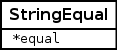
\includegraphics[]{img/StringEqual.png}
\begin{tabular}{|c|}
\hline
StringEqual \\
\hline
*equal \\
\hline
\end{tabular}
\caption[Frame Representation Example: StringEqual]{The frame representation of the \lsttext{StringEqual} structure.\label{fig:StringEqualFrame}}
\end{figure}

To represent functors and the output structure of their application, more information has to be saved. 
For one, functors have an argument, another structure on which it can depend.
To represent the result of a functor application, one needs to track which structure was passed as an argument, i.e. its frame location, as well as the values defined by the functor.
The functor has access to values inside the argument structure using the combination of frame location (\cmath{loc_{frame}}) and the index of the necessary value in the list of pointers inside that frame (\cmath{index_{val}}).

When accessing these values, the functor can only compute this index based on the values specified in the expected argument signature.
However, as mentioned in \myref{sec}{sec:Functors}, the argument structure can define more values than specified in the argument signature.
Clearly the functor should not access these values.
Yet the index of an expected value as computed from the argument signature could be different from the effective index of the corresponding value in the frame.

As a result, the view of the argument structure to the functor must be \emph{trimmed} to that specified the expected signature. 
Because the signature of the argument structure as well as the expected signature are known at compile time, this \emph{trimming} process can be performed at compile time.
The results of this trimming process can be saved in the mapping \cmath{i_{expected} \mapsto i_{effective}}.

Concluding, frames that represent the results of functor applications consist of:
\begin{enumerate}
\item Functor name
\item A pointer to the frame of the argument structure
\item The trimming map
\item The list of pointers to the values, sorted alphabetically.
\end{enumerate}
The frame representing \lsttext{StringDict} from \myref{lst}{code:DictionaryFunctor} is shown in \myref{fig}{fig:StringDictFrame}.

Because the argument structure is represented by a pointer to its corresponding frame, a functor can easily be applied to a structure that already results from functor application.
This allows iterative function application without any additional modifications.

\begin{figure}[htb]
\centering
\begin{tabular}{|c|}
\hline
StringDict \\
\hline
*StringEqual\\
*TrimMap\\
\hline
*emptyDictionary \\
*insert \\ 
*lookup \\
\hline
\end{tabular}
\caption[Frame Representation Example:StringDict]{The frame representation of the \lsttext{StringDict} structure, the output of applying functor \lsttext{DictionaryFn} to structure \lsttext{StringEqual}.\label{fig:StringDictFrame}}
\end{figure}

In order to distinguish frames that represent simple structures from those that represent structures resulting from functor application, the type of frame is tracked using a single bit right at the start of the frame.
For clarity, this value is not shown in the figures representing frames.

\subsection{Creating the Frames}
\label{sec:creatingframes}
\myref{sec}{sec:StructureOfFrames} specified how frames can represent structures.
%\to do{give functors their own chapter? Then 'The Structure of Frames' becomes a subsection with a number}
It also concluded that in order to avoid tampering with the representation of secure frames, secure frames must be located inside the protected memory of the \emph{SPM}.
This section shows that this restriction causes problems with the creation of frames representing structures.

\subsubsection{Problem Example}
When compilation is done within the context of security all secure code is compiled first, and only afterwards is the insecure context compiled.
This \emph{separate compilation} means that the compiled result of secure code is created before compilation of the insecure context starts.

For example, the earlier example of \myref{lst}{code:DictionaryFunctor} could be split up in a secure part and an insecure part as shown in \myref{lst}{code:SecureCodeFragment} and \myref{lst}{code:ContextFragment} respectively.
The code representing the functor is compiled first and separately from the code in \myref{lst}{code:ContextFragment}. 
The \emph{frame} representation for any structures defined inside \myref{lst}{code:SecureCodeFragment} can be created when compiling this file.
However, as \myref{sec}{sec:FunctorSecurityStatus} explains, any structure that results from the application of \lsttext{DictionaryFn} is supposed to be secure as well, meaning their corresponding frames should be saved in secure memory. 
Not all these applications are known when compiling \myref{lst}{code:SecureCodeFragment}.
The application of \lsttext{DictionaryFn} to \lsttext{StringEqual} inside \myref{lst}{code:ContextFragment} results in a new secure structure being created \emph{after} the secure code was compiled.

\begin{lstlisting}[frame=single,numbers=left, language=ML, caption={[Secure Code Fragment]Secure code fragment: secure.ml.},
label=code:SecureCodeFragment, morekeywords={where}]
structure StringEqual: EQUAL = 
    struct
        type t = string
        fun equal t1 t2  = case String.compare(t1,t2)
                                of EQUAL => true
                                | _ => false
    end
    
functor DictionaryFn(KeyStruct:EQUAL) :> DICTIONARY where type key = KeyStruct.t =
    struct
        type key = KeyStruct.t
        type 'a dictionary = (key * 'a) list
        val emptyDictionary = []
        fun insert d x y = (x,y)::d
        fun lookup |[] x = error
                   |(key, value):ds x = if(KeyStruct.equal key x)
                                         then value
                                         else (lookup ds x)
    end
\end{lstlisting}

\begin{lstlisting}[frame=single,numbers=left, language=ML, caption={[Insecure Context Fragment]Fragment of the insecure context: context.ml.}, label={code:ContextFragment}, morekeywords={where}]
...
structure StringDict = DictionaryFn(StringEqual);
\end{lstlisting}

As a consequence, not all frames can be created statically and added to memory at compile time.
Instead they must be added dynamically to preserve the invariant that \emph{all frames representing secure structures are located in secure memory}.
The locations of these dynamically created frames in the \emph{SPM} are kept in a list of frames, called the \emph{f-list}.

\subsubsection{Dynamically Creating Frames\label{sec:DynamicalCreationOfFrames}}
The problem described above only poses itself with functor applications: the binding of secure \lsttext{struct} expressions to a name always happens in secure code.
It's the application of a secure functor, which can happen in insecure code as well, that creates the problem.
How the dynamic creation of frames is handled depends on the location in the source language of the binding of the structure they represent to an identifier.

\begin{description}
\item[Binding in secure code:] When compiling the secure code, it is possible to create frames for all structure bindings inside the secure code, regardless whether they correspond to \lsttext{struct} expressions or functor applications.
Their frames can be added dynamically using preprocessing code located inside the \emph{SPM}. 
Since they are added by code inside the \emph{SPM}, they are guaranteed to be free from tampering.
\item[Binding in insecure code:] The bindings in insecure code require more attention when processing.
When the structure is defined using the \lsttext{struct} expression or the application of an insecure functor, the result will be an insecure structure, whose frame is allowed to be located in insecure memory.
This means that the frame can be added dynamically using preprocessing code inside the attackers context without any further considerations.

When the structure is defined by the application of a secure functor, the result is a secure structure.
This means that the frame must be saved in secure memory.
The output of compilation of the secure code is already created, so the compilation must provide a function that the context can call to create the frame.
This function corresponds nicely with the idea of \lsttext{DictionaryFn(StringEqual)} being a function from structure to structure.

For each secure functor \cmath{Fn}, the compiler adds an entry point to the \emph{SPM} to a function that allows the context to create a frame that would result from applying that functor.
This function expects two arguments: 
\begin{itemize}
\item The index in the f-list that corresponds to the frame that represents the argument of the functor, or the memory location of this frame if the argument is an insecure structure
\item The trimming map that is applied to the structure.
\end{itemize}
Using this information, the function validates its input, creates the frame in secure memory and adds it to the \emph{f-list} before returning.

The validation step is necessary because the preprocessing code is located in insecure memory.
Because this code section is not protected, these preprocessing function calls could be manipulated. 
An attacker could for example apply the functor \cmath{Fn} to a secure argument structure \cmath{S_{a}} that does not match the required signature for functor \cmath{Fn}. 
This would result in the ill-typed output structure \cmath{S_{o}}.

Structure \cmath{S_{a}} can now access values created by \cmath{S_{o}} directly, because both are located in secure code.
By choosing the unsound type assumptions that structure \cmath{S_{a}} makes carefully, this could leak information about the implementation of functor \cmath{Fn}.
As a result, when compiling a secure functor the compiler must:
\begin{itemize}
\item Add an entry point in the \emph{SPM}, pointing to a function that can create frames representing applications of the functor. 
This corresponds
\item Equip this function with the necessary checks to assure that when the argument structure is secure, the arguments signature also matches the expected signature specified by the functor definition.
In other words, code must be added that reads type information about the argument structure and checks, using structural typing as specified in \myref{sec}{sec:StructuralTyping} to ensure that functor application on secure structures only succeeds if the secure structure signature matches with the target signature.
\end{itemize}

By preserving the order in which functors are applied when adding the frames dynamically, the compiler knows at compilation time the position of every frame in the \emph{SPM}'s \emph{f-list}.
This way, the index in the f-list is a valid substitute for the real location \cmath{loc_{frame}} in memory.
\end{description}

\subsubsection{Implementing Structural Typing Checks}
In order to implement \emph{structural typing checks} when applying secure functors, knowledge about the signatures of structures must be available at runtime.
Because every secure functor has its own dedicated function that creates the frame and performs the necessary type checks, any necessary knowledge about the target signature can be hardcoded.

The signatures of structures within the \emph{SPM} are saved as meta-information linked together with the frame, called the \emph{meta-frame}.
This meta-frame tracks all type definitions and value definitions present in the signature.
It needs to formalize a target language representation of types, type definitions and value definitions.


The representation of types within the \emph{SPM} is structured as shown in \myref{fig}{fig:TypeRepresentations}.
It consists of representations for the primitive type \cmath{int}, for type variables \cmath{'a}, for types defined in other known structures and for types within the argument structure of a functor.
\begin{itemize}
\item The primitive type \lsttext{int} does not need any additional information for identification.
\item Type variables \lsttext{'a} are denoted only by an index, which says when it was declared. 
This identifies the type variables uniquely, and since type variables are matched with \emph{alpha-equivalence}, their name is not important.
\item Types \lsttext{Struct.t} defined in other known structures \cmath{S} are identified by specifying the location of the corresponding frame \cmath{F_{S}} and its index in this frames type definitions.
\item Types \lsttext{ArgStruct.t} defined in the argument structure of a functor are identified in a analogous way to types \lsttext{Struct.t}. 
They have a different identifier to mark that they depend on the argument structure, and the location of the frame in which they are defined is known only at runtime, so it is not provided.
\end{itemize}
Then, the representation of two composite types is shown, arrays \lsttext{[]} in \myref{fig}{fig:ArrayTypeRepresentation} and pairs \lsttext{(,)} in \myref{fig}{fig:PairTypeRepresentation}.

\begin{figure}[htb]
    \begin{subfigure}[b]{0.20\textwidth}
    \centering
        \begin{tabular}{|c|}
        \hline
        0 \\
        \hline
        \end{tabular}
        \caption{Type \lsttext{int}.\label{fig:IntRepresentation}}
    \end{subfigure}
    \begin{subfigure}[b]{0.20\textwidth}
    \centering
        \begin{tabular}{|l r|}
        \hline
        1 &  \gray \cmath{i_{tyvar}}\\
        \hline
        \end{tabular}
        \caption{Typevar \lsttext{'a}. \label{fig:TypeVarRepresentation}}
    \end{subfigure}
    \begin{subfigure}[b]{0.33\textwidth}
    \centering
        \begin{tabular}{|l c r|}
        \hline
        2 & \gray \cmath{loc_{frame}} & \gray \cmath{index_{type}}\\
        \hline
        \end{tabular}
        \caption{\lsttext{Struct.t}\label{fig:StructTypeRepresentation}}
    \end{subfigure}
    \begin{subfigure}[b]{0.25\textwidth}
    \centering
        \begin{tabular}{|l r|}
        \hline
        3 & \gray \cmath{index_{type}}\\
        \hline
        \end{tabular}
        \caption{\lsttext{ArgStruct.t_{i}}\label{fig:ArgTypeRepresentation}}
    \end{subfigure}
    \\
    \\
    \begin{subfigure}{0.50\textwidth}
    \centering
        \begin{tabular}{|l r|}
        \hline
        4 & \gray \cmath{type}\\
        \hline
        \end{tabular}
        \caption{Type \lsttext{[]}.\label{fig:ArrayTypeRepresentation}}
    \end{subfigure}
    \begin{subfigure}{0.50\textwidth}
    \centering
        \begin{tabular}{|l c r|}
        \hline
        5 & \gray \cmath{left_{type}} & \gray \cmath{right_{type}}\\
        \hline
        \end{tabular}
        \caption{Type \lsttext{(,)}.\label{fig:PairTypeRepresentation}}
    \end{subfigure}


    \caption[Type Representations For Metaframes]{This figure shows the representation of all different types \label{fig:TypeRepresentations}}
\end{figure}

\begin{figure}[htb]
\begin{subfigure}[b]{\textwidth}
    \centering
    \begin{tabular}{|l c c c r|}
    \hline
    name & \cmath{i_{typevar}} & \cmath{\#_{typevar}} & implementation & opacity\\
    \hline
    \end{tabular}
    \caption{Type Definition\label{fig:TypeDefinitionsRepresentation}}
\end{subfigure}
\\
\\
\begin{subfigure}[b]{\textwidth}
\centering
\begin{tabular}{|l r|}
    \hline
    name & implementation\\
    \hline
    \end{tabular}
    \caption{Value Definition\label{fig:ValueDefinitionsRepresentation}}
\end{subfigure}
\caption[Metaframe Elements]{The representation of type \textbf{(a)} and value definitions \textbf{(b)}.}
\end{figure}

The representation of type definitions is shown in \myref{fig}{fig:TypeDefinitionsRepresentation}, and that of value definitions in \myref{fig}{fig:ValueDefinitionsRepresentation}.

For the signature of an argument frame to match the target-signature, every type definition in the target signature and every value must have a match in the meta-frame, as explained in \myref{sec}{sec:StructuralTyping}:

\begin{description}
\item[Matching type definitions]
First, a match is searched for all type definitions within the target signature:
Searching inside the meta-information for a matching type definition can be done by scanning the meta-information for a type definition with the same name.
If no type definition with the same name is available, the two signatures do \emph{not} match.

If such a type definition is available, check the number of type variables \cmath{\#_{typevar}} it expects.
If the type definition in \emph{target} and \emph{candidate} signature take a different number of type variables, the two signatures do \emph{not} match.

If the matching type definitions take the same number of type variables, then the opacity of the type definition in the \emph{target} signature is of importance. If the type is \emph{not} defined opaque, the implementation of the two matching type definition is matched to ensure the same implementation.
\item[Matching values]
Next, for all values definitions inside the \emph{target} signature, a matching value definition inside the \emph{candidate} signature is identified using the names.
In this matching, only the values which correspond to a result of the \emph{trimming map} are considered.

When a name match is found, its type is checked.
When creating a meta-frame, any type used in the typing of values is substituted by its implementation up until the first opaque type is encountered.
This ensures that checking whether the type of two values match can be done by checking that either the type stated in the candidate signature is exactly the same as the type in the target signature, or it is a type variable that substitutes \emph{consistently} for the type listed in the target signature.
\end{description}

\subsubsection{Creating Meta-Frames}
Implementing \emph{structural typing} required knowledge about the signatures of structures to be available at runtime.
It introduced \emph{meta-frame}s as a type of meta-information linked together in memory with the frame.
These \emph{meta-frame}s track all type definitions and value definitions present in the structures signature.

The content of these \emph{meta-frame}s can mostly be determined at compile time. This surely is the case for structures, but it also is the case for functors that are not modified by a \lsttext{where} expression.
This means that the function that creates a frame corresponding to a functor application can largely hardcode the content of the corresponding meta-frame.
When creating a meta-frame, any type used in the typing of values is substituted by its implementation up until it contains only opaque types, counting \lsttext{int} as an opaque type.

\begin{description}
\item[Handling where Expressions] 
Only \lsttext{where} expressions of the template \lsttext{where type t = ArgStruct.t'} can not be processed at compile time.
For these expressions, the compiler slightly modifies the matching algorithm so that it checks
\begin{enumerate}
\item That the implementation of type \lsttext{t} is in fact \lsttext{ArgStruct.t}.
\item What the opaqueness and implementation of type \lsttext{ArgStruct.t} is, so that any reference to type \lsttext{t} or \lsttext{ArguStruct.t} can be substituted by its implementation.
\end{enumerate}
\end{description}
\subsection{Calling Structure Values}
Access to any value of a source language structure is uniquely determined in the target language using the location (\cmath{loc_{frame}}) of the frame in memory and the index of the value (\cmath{index_{val}}) in its list of value pointers.

In the source language, all values are either accessible across the security boundary or strictly accessible only within the same structure, so the same must hold for the target language.
It is easy to make values accessible only from within the same structure: they are not given an entry within the list of value pointers, and their location is not made into an entry point for the \emph{SPM}.

All other values are accessible across the security boundary. However, as frames are saved in the memory corresponding to its security status, the attackers context is not able to access frames corresponding to structures within the \emph{SPM} directly.
Worse, the attackers context is not even allowed to know the exact location \cmath{loc_{frame}} of these secure frames.

%To solve this, all $loc_{frame}$ are masked by inserting them into a list of frames, called the \emph{f-list}, in the order of their definitions.
This is solved by inserting all \cmath{loc_{frame}} into the \emph{SPM}'s list of frames (\emph{f-list}) that was introduced in \myref{sec}{sec:DynamicalCreationOfFrames}. 

Frames that were created in secure code are sorted alphabetically by the identifier they were bound to and put in the \emph{f-list} first.
This alphabetical ordering is necessary because changing the order of structure bindings does not break contextual equivalence at the high-level \MiniML\ language.
The frame locations of frames created in insecure code are appended in the order of their definitions.
This means that the specific mapping of an identifier to value of its index is known statically.

%\to do{Sort those bound in secure memory alphabetically, and append those bound to an identifier in insecure context in the order of their definition! Otherwise, contextual equivalence is broken, isn't it?}
%TO DO: Doesn't this break contextual equivalence? Solution: Sort alphabetically for those created in secure memory!
Anywhere a secure structure is used in the source language, it is represented by the \cmath{loc_{frame}} pointer or its masking index in the \emph{f-list}.

To allow context code to access values from secure structures, a wrapper function is provided that is located inside the \emph{SPM}.
This wrapper function corresponds to an \emph{entry point} to the \emph{SPM}.
The context can now pass an index in the \emph{f-list} \cmath{index_{f-list}} and an index for the structure value \cmath{index_{val}}, as well as any arguments that should to be passed to the value to this wrapper function.
%to do: alternatively the pointer to the value is passed directly
This wrapper, because it is located in secure code, can access the \emph{f-list} and the frames themselves.
It then does the following things:
\begin{itemize}
\item Check whether \cmath{index_{f-list}} corresponds to a real frame by using the expected length of the list.
Since structures resulting from a functor application are added dynamically, a situation could arise where the corresponding frame has not yet been added, or where something went wrong while adding the frame.
In this case the wrapper function must not allow the \cmath{index_{f-list}} to be used.
\item Use \cmath{index_{f-list}} to get a \cmath{loc_{frame}} for the correct frame.
\item Check whether the frame represents a simple structure or the result of functor application.
\item Look up \cmath{index_{val}} in the list of pointers within the frame to get a pointer to the accessed value.
\item Call this value with any relevant arguments.
In case the frame represents the result of functor application, the pointer to the frame must be provided as a parameter when calling the value.
The function implementing the value will uses this frame to determine the argument frame.
%argument frame must be provided when calling the value.
%By design, a pointer to this frame is always present within the frame representing the functor output itself.
\item return any results to the caller.
\end{itemize}

The wrapper functions only as a wrapper, so it presumes any clearing of flags, registers, masking of values or other precautionary measures have already been taken care of by the functions that it wraps.

Since all structure values are accessible through this wrapper function, the separate structure value stubs do \emph{not} have to be entry points in the \emph{SPM}. The wrapper function will always be necessary, because insecure functors that call a value in their argument structure can not hardwire a specific entry point in their generic code.
\\[1em]
\label{sec:StaticDefinitionFunctorApplication}
Indeed, the stubs corresponding to structure values even \emph{cannot} be made entry points in the \emph{SPM}, because the source language context is oblivious to whether a structure bound in secure code was the result of a functor application, or was statically defined. This corresponds to \myref{lst}{lst:FunctorApplicationOrStaticDefinition1} being contextually equivalent to \myref{lst}{lst:FunctorApplicationOrStaticDefinition2}.

\begin{lstlisting}[frame=single,numbers=left, language=ML, caption={[Functor Application or Static Definition: 1]Binding StrA and StrB using functor application.},
label=lst:FunctorApplicationOrStaticDefinition1, morekeywords={where}]
functor F(ArgStruct:ArgSig) :> OutputSig =
    struct
        val x = ArgStruct.f x
    end
    
structure StrA = F(Arg1)
structure StrB = F(Arg2)
\end{lstlisting}

\begin{lstlisting}[frame=single,numbers=left, language=ML, caption={[Functor Application or Static Definition: 2]Binding StrA and StrB using both static definition and functor application.},
label=lst:FunctorApplicationOrStaticDefinition2, morekeywords={where}]
functor F(ArgStruct:ArgSig) :> OutputSig =
    struct
        val x = ArgStruct.f x
    end
    
structure StrA :> OutputSig =
    struct
        val x = Arg1.f x
    end

structure StrB = F(Arg2)
\end{lstlisting}


If stubs were made entry points in the target language, the difference between static definition and function application would break contextual equivalence.
\begin{itemize}
\item Compiling \myref{lst}{lst:FunctorApplicationOrStaticDefinition1} means calling value \lsttext{StrA.x} would use the same entry point as calling \lsttext{StrB.x}.
\item Compiling \myref{lst}{lst:FunctorApplicationOrStaticDefinition2} means calling value \lsttext{StrA.x} would use an entry point different from the one used when calling \lsttext{StrB.x}
\end{itemize}
Clearly, this would result in \myref{lst}{lst:FunctorApplicationOrStaticDefinition1} and \myref{lst}{lst:FunctorApplicationOrStaticDefinition2} not being contextually equivalent in the target language.

%However, in order to allow optimization, the structure values could safely be made entry points of the \emph{SPM} with only minimal changes to the scheme above:
%\begin{itemize}
%\item The high-level language context is oblivious to whether a structure bound in secure code is the result of functor application or was statically defined.
%As a result, when the stubs that access a structure value are made entry points to the \emph{SPM}, all stubs must take a frame location as an extra argument.

%\item When all stubs must take a frame location as an extra argument, the frame location can no longer be that of the argument structure because statically defined structures do not have an argument structure. Instead, the passed frame location must be the location of the \emph{own} frame.
%When the stub represents a value of a functor, 
%\end{itemize}

%The values within a structure resulting from functor application are stubs that expect an extra argument, the location of the \emph{own} frame.
%If these stubs can be called directly by the context without the wrapper function, care must be taken to check that the location of the own frame is either inside insecure memory or is interpreted as a mask in the f-table.

%When providing this optimization, structures that were defined statically, i.e. \emph{not} as a result of functor application, need to take the location of their extra argument 


% is able to read the pointer corresponding to the $(loc_{frame}, index_{val})$ pair and call the necessary value.
%It can then return any results to its caller.

%If the values are inside a structure resulting from functor application, care has to be taken.
%The code representing the values expects the frame of the argument structure to be passed as a first argument.
%By design, a pointer to this frame is always present within the frame representing the functor output itself.

\subsection{Security Consequences}

In order to explore the possibility of contextual equivalence breaking due to the representation of structures differing between source and target language, the possible combinations of functor and structure security and the relevant security measures are recapped here case by case.
%Since functor application results in a structure as well, these structures must also be representable as frames.
%In order to allow this, frames consist of a type indicator that identifies it as a structure defined using the struct keyword, or a structure resulting from functor application.

%to do: Trimming problem, problem with iterated functor applying. (When applying a secure functor, the resulting structure must be saved in the list of structures in secure memory. This consists of a pointer to the functor
%to do: suppose functor application is done in the insecure code. Structure is in secure code. Regardless of where the functor is located, the linker knows what signature it expects and can trim down the 
%Origin problem: What is the origin of the structure. Is it a pointer in the insecure memory, or is it a masking index?
%Fresh type names at every application, even to the same arguments! http://books.google.be/books?id=oPaAAahVu_kC&pg=PA345&lpg=PA345&dq=functors+sml+each+new+application+provides+fresh+types&source=bl&ots=g-VRLSeChc&sig=v4t4Ch42F-pktGaLpqgMq51K92k&hl=en&sa=X&ei=YvfGU92vHYrR7Aa89oGoDw&ved=0CCsQ6AEwAQ#v=onepage&q=functors%20sml%20each%20new%20application%20provides%20fresh%20types&f=false
%note whether the application was really performed!
\begin{description}
\item[Secure functor and secure structure] 
%In this case, at the moment of functor application a new frame is created representing the result of this functor application. This consists of 
The \emph{frame} representing a structure is located in the same part of memory as the structure was defined.
Since in this combination both the functor code and the frame are located inside protected memory, no tampering is possible.
When functor code is called with a reference to the frame in secure memory, the functor code is able to read the frame directly, because the functor is part of the \emph{SPM}. It can then call any value of the argument structure using the pointer provided by the frame.

If the application of the secure functor is done inside insecure code, the frame creating function corresponding to this functor must be called, and the types are checked dynamically using type information in the \emph{meta-frame}.
\item[Secure functor with insecure structure]
When a secure functor is applied to an insecure structure, its result is a secure structure that calls functions provided by the insecure structure.
The resulting structure \emph{depends} on the insecure structure.
It must call these functions using the same precautions as regular callbacks to the attacker's context.
Of course the pointers that represent these functions can be manipulated by the attacker because the frame is now located in insecure memory.
However, because contextually equivalent implementations of the functor must perform the same callbacks with the same arguments in the source language in the same order, their target language versions will always use the same value pointers provided by the insecure frame, with the same parameters in the same order.
As a result, the regular precautions, such as clearing registers, switching the stack and masking values that pass from secure code to the insecure context, are sufficient to ensure preservation of contextual equivalence of the functors in the target language.

If the application of the secure functor is done inside insecure code, the frame creating function corresponding to this functor must be called, and the types are checked dynamically using type information in the \emph{meta-frame}.
%to do: OR depends on values
\item[Insecure functor with insecure structure]
In this case, both the functor code and the frame are located inside unprotected memory.
The structure that results from the application is considered to be part of the attacker's context.
The use of values from the insecure structure by code inside the insecure functor can happen without any security precautions, as the expected behavior is simply equivalent to that of an unparametrized structure in the attacker's context that depends on another structure of this same context.
\item[Insecure functor with secure structure]
Because the code of the functor is now located outside of the \emph{SPM}, special care needs to be taken when the functor depends on values provided by the structure.
Because the frame \cmath{Fr_{s}} representing the structure is now in secure memory, the functor cannot manipulate this frame or perform reads on this frame.
In order for insecure functors to call these functions, a generic wrapper is provided by the \emph{SPM} that takes as argument a \cmath{loc_{frame}} and an \cmath{index_{val}}, as well as any arguments that would otherwise be passed directly.
As a result, the generic wrapper returns the result of the call to its caller.
%to do: possible variant: this generic entry point returns a pointer
%As a result, a pointer to the correct entry point is returned to the insecure code, which it can then call with the necessary arguments.
%todo
\end{description}

%\to do{When calling values of the argument structure, the functor must at all times take care to determine whether the argument frame represents another functor output, or a basic structure, since calling a value within functor output requires the first argument to be a frame pointer to the argument structure. Should I add this remark in text, or should I provide code that does this check, and refer to that.}

\section{Conclusion}
In this chapter, some more advanced concepts of ML were added to the \MiniML\ language:

Higher order functions, and the closely related concept of closures, can be introduced if certain sensitive information, such as environment values and pointer values are confined to the secure memory.
This is done by reusing the earlier concept of \emph{masking}\cite{Patrignani}, and applying it to closures.
In order to execute these closures, a \emph{closure-evaluation entry point} was introduced.

Functors were added by introducing the \emph{target} language concept of a \emph{frame} that represents structures.
Implementing values defined by functors using stubs that expect an argument representing the parameter structure makes generic translation of these values in the \emph{target} language possible.
The dichotomy between the security status of an output structure and where the functor application generating the structure is located results in the \emph{dynamic} creation of \emph{frames} and the added difficulty of \emph{structural type checking} functor applications.
This is solved by adding meta information in so called \emph{meta-frame}s capturing any necessary information of types.

Because functors can exist in insecure code, they can be passed frames. These frames are \emph{masked} in the same way as closures, which calls for another \emph{wrapping function} to be made available as an entry point into the \emph{SPM}, so that the values within frames are callable.
\chapter{Advanced Concepts: Formalization}
\label{chap:FormalizationOfAdvancedConcepts}
First, \myref{sec}{sec:formalspec2} of this chapter extends the formalization of \MiniML\ made in \myref{sec}{sec:MiniMLFormalSpecification} with the additions described in \myref{chap}{chap:AdvancedConcepts}.
Later, \myref{sec}{sec:formalizedcompiler2} extends upon the secure compiler as it was formalized in \myref{sec}{sec:formalizedcompiler}.

\section{Formal Specification of \MiniML}
\label{sec:formalspec2}
The \MiniML\ language as specified in \myref{chap}{chap:formalspecification} consisted of a very limited subset of the ML language.
In \myref{chap}{chap:AdvancedConcepts}, this issue was addressed by adding two more concepts to the subset:
\begin{description}
\item[Higher-order functions]
The concept of \emph{higher-order functions} allows that functions receive other functions as their input, or return functions as their output.
By allowing them to be assigned as a value to a variable, functions essentially become \emph{first-class values}, going by the name \emph{closure}.

To implement closures, the ability to create anonymous functions using the $\lambda$ notation is added.
This addition makes it possible to define a function as: \cmath{\lambda(\overline{x}:\overline{\sigma}).e}.
This expression is considered as the construction of a closure.

These expressions are also the \emph{only} way of constructing a closure, as explained in \myref{sec}{sec:OnlyLambdaClosures}. 
Essentially, when a named function is used as a closure, this is considered to be syntactic sugar.
Its desugared form is an expression in which a closure is explicitly constructed using the $\lambda$-notation to wrap around the named function.

\item[Functors]
The idea of functors is that they act as functions from structures to structures.
They provide a way to parametrizing structures.

A parametrized structure is a functor \cmath{F} that, instead of depending on another structure \cmath{Str_{2}} by name, receives this structure as an argument.
To ensure that the structure given as an argument defines the necessary bindings, the argument structure is restricted by a signature \cmath{Sig}.
The functor definition defines all bindings of the parametrized structure.
In short, the definition of a functor corresponds to \lsttext{functor $\ \cmath{id}$($\cmath{ArgStr:Sig_{1}}$):>$\cmath{Sig_{2}}$ = struct $\ \overline{d}$ end}.

The application of a functor \cmath{F} to a \cmath{Str_{1}}, written as \cmath{F(Str_{1})} then results in a new structure \cmath{Str_{2}} that can be bound to an identifier.
This resulting structure, or \emph{output} structure, can be used like any regular structure. Any time the functor bindings uses \cmath{ArgStr.x}, \cmath{Str_{2}} uses \cmath{Str_{1}.x}.
\end{description}

These additions have important consequences for the way \MiniML\ is compiled.
To be able to describe these consequences, the formalization of \MiniML\ as given in \myref{chap}{chap:formalspecification} is revisited.

\subsection{Syntax}
The additional concepts introduce some new syntactical constructs to the \MiniML\ syntax.
The additions to the Core syntax are seen in \myref{fig}{fig:UpdatedCoreSyntax}, additions to the Module syntax in \myref{fig}{fig:UpdatedModuleSyntax}.
The Program syntax remains unchanged by the additions from \myref{chap}{chap:AdvancedConcepts}.

\subsubsection{Closures}
Closures introduce the \cmath{\lambda}-expression to the Core syntax, \myref{fig}{fig:UpdatedCoreSyntax}.
It specifies a number of argument, their identifiers and their types, as well as the expression that represents the function body.

\begin{figure}[htb]
\caption[Updated Core Syntax]{The Module Syntax, updated from {\protect\myref{fig}{fig:CoreSyntax}}.\label{fig:UpdatedCoreSyntax}}
\end{figure}
\vspace{-1em} %Todo: LaTeX voodoo
\subsubsection{Functors}
Functors introduce the functor definition and functor application as module expressions to the Module syntax \myref{fig}{fig:UpdatedModuleSyntax}.

A functor definition specifies:
\begin{itemize}
\item the functor identifier,
\item the identifier \cmath{ArgStr} for the argument structure,
\item the signature \cmath{Sig_{1}} to which the argument structure must comply,
\item the signature \cmath{Sig_{2}} to which the functor's body must comply,
\item and the body \cmath{\overline{d}}.
\end{itemize}
A functor application specifies the identifier to which the resulting structure is bound, the functor identifier, and the identifier for the structure that is passed as an argument.
\begin{figure}[htb]
\caption[Updated Module Syntax]{The Module Syntax, updated from {\protect\myref{fig}{fig:ModuleSyntax}}.\label{fig:UpdatedModuleSyntax}}
\end{figure}

\subsection{Type system}
The type system also needs some minor modifications to account for the new concepts.
As earlier, due to its simplicity the Program type system sees no modifications.

First, the concept of a \emph{context} $\Gamma$ is extended in \myref{fig}{fig:UpdatedMiniMLContexts}, so that it can contain assumptions related to functors: The signature it conforms to, its body of definitions, and the name of the signature that its argument must conform to.

\begin{figure}[!htb]
\begin{align*}
\begin{aligned}
\text{Context }\\
\Gamma ::=\; & \ldots \\ 
&| \; (\mathit{FunId} \mapsto \lbrace \Sigma, \overline{d}, SigId\rbrace), \Gamma
                                           & \expl{(functor definition)}
\end{aligned}
\end{align*}
\caption[Updated Contexts]{Contexts in the MiniML type system, extending \earlier{fig}{fig:MiniMLContexts}.}
\label{fig:UpdatedMiniMLContexts}
\end{figure}

Next, the typing rules are updated, as shown in \myref{fig}{fig:UpdatedTypeRulesCore} and \myref{fig}{fig:UpdatedTypeRulesModule}.

\subsubsection{Closures}
The addition of closures, as a Core concept, modifies the function application rule T-App inside the Core typing system in \myref{fig}{fig:UpdatedTypeRulesCore}, so that it allows arguments or return values to be of the function type.
It also adds the $\lambda$-expression typing rule T-Lambda. 
This rule describes that a $\lambda$-expression is well typed if its defining expression can be typed to the result type, assuming each argument is of the stated argument type.

\begin{figure}[htb]
\begin{align*}
\tag{T-App}
&\frac
{\Gamma \vdash e_{1}:\overline{\tau_{2}} \rightarrow \tau_{1}
    \longspace
    \Gamma \vdash \overline{e_{2}}:\overline{\tau_{2}}}
{\Gamma \vdash e_{1} \overline{e_{2}}:\tau_{1}}
\\[1em]
\tag{T-Lambda}
&\frac
{\overline{(x:\tau_{2})} \cup \Gamma \vdash e : \tau_{1}}
{\Gamma \vdash \lambda\ \overline{x}.e : \overline{\tau_{2}} \rightarrow \tau_{1}}
\end{align*}
\caption[Updated Typing Rules: Core Language]{Updated typing rules for the Core language, extending \earlier{fig}{fig:TypeRulesCore}. \label{fig:UpdatedTypeRulesCore}}
\end{figure}

\subsubsection{Functors}
Functors are strictly a Module language concept, which means modifications are limited to Module language, updated in \myref{fig}{fig:UpdatedTypeRulesModule}.
It adds two rules:
\begin{description}
\item[T-FunctorDef]
A rule to type a functor definition.
This rule says that the \emph{principal signature} of the body (\cmath{PS(\overline{d})}) must match with the signature specified in the ascription of the functor.
Furthermore, each definition in the body must be correctly typed, assuming the well-typedness of all other definitions and the values defined in the argument structure. 
\item[T-FunctorApp]
A rule that types functor applications.
This rule says that a functor application is well typed if the effective signature of the structure that was passed as an argument matches to the expected signature.
Furthermore, it specifies that the structure is saved in the context.
The output structure's identifier maps to the result signature of the functor and the body of the functor after substituting all references to the argument structure.
\end{description}


\begin{figure}[htb]
\begin{align*}
%&\Gamma \vdash true : bool \tag{T-True} \\
%&\Gamma \vdash false : bool \tag{T-False} \\
&\Gamma \vdash num \; n : nat \tag{T-Num}
\\[1em]
\tag{T-Mono}
&\frac{\sigma_{2} \geq \sigma_{1} \longspace id:\sigma_{2} \in \Gamma}{\Gamma \vdash id:\sigma_{1}}
\\[1em]
\tag{T-App}
&\frac{\Gamma \vdash e_{1}:\overline{\tau_{2}} \rightarrow \tau_{1} \longspace \Gamma \vdash \overline{e_{2}}:\overline{\tau_{2}} \longspace \tau_{1} \neq \tau_{3} \rightarrow \tau_{4} \longspace \forall \tau \in \overline{\tau_{2}} : \tau \neq \tau_{3} \rightarrow \tau_{4}}
{\Gamma \vdash e_{1} \overline{e_{2}}:\tau_{1}}
\\[1em]
%\tag{BuildContext1}
%& id:\sigma \rightarrow \emptyset, (id:\sigma) \\ \\
%\tag{BuildContext2}
%%&\frac{p_{1}:\sigma_{1} \rightarrow \Gamma_{1} \longspace p_{2}:\sigma_{2}\rightarrow \Gamma_{2}}
%{(p_{1},p_{2}):\sigma_{1}\times \sigma_{2} \rightarrow \Gamma_{1}\cup \Gamma_{2}} \\ \\
%\tag{T-Fun}
%&\frac{p:\tau_{2} \rightarrow \Gamma_{2} \longspace \Gamma_{2} \cup \Gamma_{1} \vdash e:\tau_{1}}
%{\Gamma_{1} \vdash \lambda(p:\tau).e:\tau_{2} \rightarrow \tau_{1}} \\ \\
%
%\tag{T-IfThenElse}
%&\frac{\Gamma \vdash e_{1}:bool \longspace \Gamma \vdash e_{2}:\tau \longspace \Gamma \vdash e_{3} : \tau}
%{\Gamma \vdash if \; e_{1} \; then \; e_{2} \; else \; e_{3} : \tau} \\ \\
%
%\tag{T-Pair}
%&\frac{\Gamma \vdash e_{1}:\tau_{1} \longspace \Gamma \vdash e_{2}:%\tau_{2}}
%{\Gamma \vdash (e_{1},e_{2}) : \tau_{1}\times\tau_{2}} \\ \\
%\tag{T-PairLeft}
%&\frac{\Gamma \vdash p:\tau_{1}\times\tau_{2}}
%{\Gamma \vdash \mathit{p.left} : \tau_{1}} \\
%\\
% \tag{T-PairRight}
%&\frac{\Gamma \vdash p:\tau_{1}\times\tau_{2}}
%{\Gamma \vdash \mathit{p.right} : \tau_{2}} \\
%\\
\tag{T-Let}
&\frac{\Gamma \vdash e_{2}:\sigma \longspace \Gamma, x:\sigma \vdash e_{1}:\tau}
{\Gamma \vdash let\;p\;=\;e_{2}\;in\;e_{1}:\tau}
\\[1em]
\tag{T-Gen}
&\frac{\Gamma \vdash e:\sigma \longspace \alpha \not\in \mathit{free(\Gamma)}}{\Gamma \vdash e : \forall \alpha . \sigma}
\\[1em]
\tag{T-Pair}
&\frac
{\Gamma \vdash e_{1}:\tau_{1} \longspace \Gamma \vdash e_{2}:\tau_{2})}
{\Gamma \vdash (e_{1},e_{2}):\tau_{1} \times \tau_{2}}
\\[1em]
\tag{T-List}
&\frac
{\Gamma \vdash e_{1}:\tau \longspace \Gamma \vdash e_{2}:[\tau]}
{\Gamma \vdash e_{1}::e_{2}:[\tau]}
\\[1em]
\tag{T-EmptyList}
&\Gamma [] : \forall \alpha.[\alpha]
\\[1em]
\tag{T-PairLeft}
&\frac
{\Gamma \vdash e:\forall \alpha . \tau \times \alpha}
{\Gamma \vdash e.\#1:\tau}
\\[1em]
\tag{T-PairLeft}
&\frac
{\Gamma \vdash e:\forall \alpha . \alpha \times \tau}
{\Gamma \vdash e.\#2:\tau}
\end{align*}
\caption[Updated Typing Rules: Core Language]{Updated typing rules for the Core language. \label{fig:UpdatedTypeRulesCore}}
\end{figure}

\begin{figure}[htbp]
\begin{align*}
\tag{T-Signature}
&\Gamma \vdash SigId = \Sigma \rightarrow (\mathit{SigId} \mapsto \Sigma),\Gamma
\\
\\
\tag{T-Structure}
&\frac
{\Gamma[SigId].\Sigma \succeq \mathit{PS}(\overline{d}) \longspace PS(\overline{d}) \cup \Gamma \vdash \overline{d}}
{\Gamma \vdash StrId : SigId = \overline{d} \rightarrow (\mathit{StrId} \mapsto \lbrace \mathit{ES}(\overline{d}), \overline{d}\rbrace),\Gamma}
\\
\\
\tag{T-ValDef}
&\frac
{\Gamma \vdash e:\tau}
{\Gamma \vdash \text{\lsttext{val}}\ \mathit{id} = e:\tau}
\\
\\
\tag{T-FunDef}
&\frac
{\overline{(x = \tau_{2})} \cup \Gamma\ \vdash e:\tau_{1}}
{\Gamma \vdash \text{\lsttext{fun}}\ \mathit{id}\ \overline{x}= e:\overline{\tau_{2}} \rightarrow \tau_{1}}
\\
\\
\tag{T-TypeDef}
&\frac
%{\forall \alpha_{i} \in \overline{\alpha} : \alpha_{i} \in \tau}
{\overline{\alpha} = \mathit{free(\tau)}}
{\Gamma \vdash \text{\lsttext{type}}\ \overline{\alpha}\ t = \tau}
%\\
%\\
%\tag{T-Structure-opaque}
%&\frac
%{\Gamma[SigId].\Sigma \succeq PS(\overline{d})}
%{\Gamma \vdash StrId :> SigId = \overline{d} \rightarrow (\mathit{StrId} \mapsto \lbrace%\Gamma[SigId].\Sigma, \overline{d} \rbrace ),\Gamma}
\\
\\
\tag{T-ModVar}
&\frac
{StrId.id:\sigma \in \Gamma[StrId].\Sigma}
{\Gamma \vdash \mathit{StrId.id} : \tau}
\\
\\
\tag{T-ModTransType}
&\frac
{\Gamma \vdash e:\sigma_{1} \longspace t\ \overline{\alpha} = \sigma_{2} \in \Gamma[\mathit{StrId}].\Sigma \longspace \sigma_{2} \geq \sigma_{1}}
{\Gamma \vdash e : \mathit{StrId.t}\ \overline{\tau}}
\\
\\
\tag{T-ModTransType2}
&\frac
{\Gamma \vdash e:\mathit{StrId.t}\ \overline{\tau} \longspace t\ \overline{\alpha} = \sigma_{2} \in \Gamma[\mathit{StrId}].\Sigma \longspace [\bigcup_{\tau_{i} \in \overline{\tau}} \alpha_{i} \mapsto \tau_{i}]\sigma_{2} = \sigma}
{\Gamma \vdash e:\sigma}
%This rule says that if an expression evaluates to a StrId.t type in an expression, the type must be transparent, or it must come from StrId.id with that type.
%\\
%\\
%&\frac{
%\emptyset \vdash \overline{d}\rightarrow \Gamma' }
%{PS(\overline{d})} \\
\end{align*}
\caption[Updated Typing Rules: Module Language]{Updated typing rules for the Module language. \label{fig:UpdatedTypeRulesModule}}
\end{figure}


%\begin{figure}
%\begin{align*}
%%\\ \\
%%\tag{T-Letrec}
%%&\frac{\Gamma \vdash let\;p\;=\;\mathit{fix}\;(\lambda p.e_{2})\;in\%;e_{1}:\tau}
%%{\Gamma \vdash letrec\;p\;=\;e_{2}\;in\;e_{1}:\tau} \\ \\
%%\tag{T-Fix}
%%&\frac{\Gamma \vdash e : \tau \rightarrow \tau}
%%{\Gamma \vdash \mathit{fix\;e} : \tau} \\
%%\displaybreak
%\\
%\tag{T-ModVarThis}
%&\frac{\sigma \geq \tau \longspace this.id:\sigma \in \Gamma}
%{\Gamma \vdash this.id : \tau} \\ 
%\\
%\tag{T-ModVarOther}
%&\frac{
%\Gamma \vdash M_{i}
%\longspace id:\tau \in \Gamma[M_{i}].\Sigma}
%{\Gamma \vdash \mathit{M_{i}.id} : \tau} \\
%\\
%%\tag{T-FunctorVar}
%%&\frac{\overline{\Gamma \vdash M_{1..n}}
%%\longspace
%%\overline{\Sigma_{3} \succeq \Gamma[M_{1..n}].\Sigma}
%%\longspace
%%\Gamma \vdash F_{i}(\overline{M_{1..n}})
%%\longspace
%%id:\tau \in \Gamma[F_{i}].\Sigma_{1}}
%%{\Gamma \vdash \mathit{F_{i}(\overline{M_{1..n}}).id}:\tau} \\
%%\\
%\tag{T-Module}
%&\frac{
%\emptyset \vdash \Gamma[M_{i}].\overline{d}\rightarrow \Gamma' \longspace \Gamma' \vdash \Gamma[M_{i}].\Sigma_{i}}
%{\Gamma \vdash M_{i}} \\
%\\
%%\tag{T-Functor}
%%&\frac{
%%\emptyset \vdash [\overline{M_{1..n} \mapsto M_{arg}}]\overline{d} \rightarrow \Gamma' \longspace \Gamma' \vdash \Gamma[F_{i}].\Sigma}
%%{\Gamma \vdash F_{i}(\overline{M_{args}})}\\
%%\\
%\tag{T-ModInterfaceField}
%&\frac{(x:\tau) \in \Gamma \longspace \Gamma \vdash \Delta}
%{\Gamma \vdash (x:\tau),\Delta}\\
%\\
%\tag{T-ModInterfaceModule}
%&\frac{(M=\lbrace \Sigma_{2}, \overline{d} \rbrace^{M}) \in \Gamma
%\longspace \Sigma_{1} \succeq \Sigma_{2} 
%\longspace \Gamma \vdash \Delta}
%{\Gamma \vdash (M:\Sigma_{1}),\Delta}\\
%\\
%\tag{T-ModBodyV}
%&\frac{ (x:\tau),\Gamma \vdash \overline{d} \rightarrow \Gamma' \longspace \Gamma \vdash e:\tau}
%{\Gamma \vdash (x=e:\tau),\overline{d} \rightarrow (x:\tau),\Gamma'} \\
%\\
%\tag{T-ModBodyM}
%&\frac{\Gamma \vdash \lbrace\Sigma, \overline{d} \rbrace^{M_{i}} }
%{\Gamma \vdash (\mathit{M_{i}=\overline{d}}:\Sigma),\overline{d} \rightarrow (M_{i}=\lbrace \Sigma,\overline{d} \rbrace),\Gamma'} \\
%\\
%\tag{T-EmptySet}
%&\frac{\Gamma \vdash \Diamond}
%{\Gamma \vdash \emptyset}
%\end{align*}
%\caption{Typing rules for the Module language. \label{fig:TypeRulesModule}}
%\end{figure}

\subsection{Operational Semantics}
The updated formalization of \MiniML\ is concluded with a description of the updates to the operational semantics.

Fist, the concepts of values v is extended in \myref{fig}{fig:UpdatedValues} to reflect the addition of closures as a \emph{first class value}.
A closure is a pair, consisting of an expression and an environment in which this expression is evaluated.
The environment consists of a set of bindings of identifiers to values, as shown in \myref{fig}{fig:Environments}.

\begin{figure}[htb]
\begin{align*}
\text{Value }v ::=\;& \ldots \\
&| (e, \rho)\ 
\end{align*}
\caption[Updated Value Concept]{Updated concept of `values', extending \earlier{fig}{fig:MiniMLOperationalSemanticEntitiesAndRelations}.\label{fig:UpdatedValues}}
\end{figure}

\begin{figure}[htb]
\begin{align*}
\text{Environment }\rho ::=\;& \emptyset \\
&| (x \mapsto v), \rho\ 
\end{align*}
\caption[Environment entity]{Environments.\label{fig:Environments}}
\end{figure}

Next, the concept of the module table T is extended, as shown in \myref{fig}{fig:UpdatedModuleTable} so that it can keep track of the definitions of functors.
The module table maps functor identifiers to their body of definitions.

\begin{figure}[htb]
\begin{align*}
\text{Module Table } T\; ::= \;& \ldots \\
&| \; \cmath{(FunId) \mapsto \overline{d}}, T
\end{align*}
\caption[Updated Module Table Concept]{Updated concept of a `module table', extending \earlier{fig}{fig:MiniMLOperationalSemanticEntitiesAndRelations}.\label{fig:UpdatedModuleTable}}
\end{figure}

\subsubsection{Closures}
The addition of closures adds two evaluation rules, one concerning their definition and one for their application, shown in \myref{fig}{fig:ClosureEvaluationRules}.
\begin{description}
\item[E-ClosureDef]
This rule describes how a $\lambda$-expression is evaluated.
The $\lambda$-expression creates a closure value, consisting of the expression $e$ and the environment.
The environment contains bindings for all variables used in the defining expression~$e$, but not defined within the expression. These are called the non-local of free variables of e, defined as \cmath{FreeVar(e)}.
\item[E-ClosureApplication]
This rule describes how the evaluation of a closure happens.
When the first expression of regular function application is evaluated to a closure value, it the function application is evaluated to the defining expression with all the arguments identifiers substituted with their values, and all mappings inside the environment applied.
\end{description}

\begin{figure}[htb]
\begin{align*}
\tag{E-ClosureDef}
&\frac
{\rho = \cmath{FreeVar(e)}}
{T \vdash \lambda \overline{x}.e \rightarrow T \vdash (e,\rho)}
\\
\\
\tag{E-ClosureApplication}
&\frac
{T \vdash e_{1} \rightarrow T \vdash (e_{2}, \rho)}
{T \vdash e_{1} \overline{v} \rightarrow [\overline{x} \mapsto \rho \cup \overline{v}] e_{2}}
\end{align*}
\caption[Closure Evaluation Rules]{The evaluation rules concerning closures, extending on \earlier{fig}{fig:MiniMLOperationalSemantics}. \label{fig:ClosureEvaluationRules}}
\end{figure}


\subsubsection{Functors}
Adding functors to the language means there must be a way to evaluate functor definitions and functor applications.
This means the additions of functors introduces two evaluation rules, as described in \myref{fig}{fig:FunctorEvaluationRules}
\begin{description}
\item[E-FunctorDef]
When a functor definition is encountered, a mapping from the functor identifier to its definition body should be saved in the module table T.
\item[E-FunctorApp]
When a structure is bound by a functor application, a mapping for the structure identifier is added in the module table T.

\end{description}

\begin{figure}[htb]
\begin{align*}
\tag{E-FunctorDef}
&\cmath{T \vdash FunId(ArgStr:SigId_{1}) = \overline{d}, P \rightarrow (FunId \mapsto \overline{d}), T \vdash P}
\\
\\
\tag{E-FunctorApp}
&\cmath{T \vdash StrId_{1} = FunId(StrId_{2}), P \rightarrow (StrId_{1} \mapsto [ArgStr \mapsto StrId_{2}]\overline{d}), T \vdash P}
\end{align*}
\caption[Functor Evaluation Rules]{The evaluation rules concerning functors, extending on \earlier{fig}{fig:MiniMLOperationalSemantics} and \myref{fig}{fig:ClosureEvaluationRules}. \label{fig:FunctorEvaluationRules}}
\end{figure}


\section{Formalized Compiler}
\label{sec:formalizedcompiler2}
This section adapts the secure compiler formalized in \myref{sec}{sec:formalization} to the security measures and concerns introduced with the addition of closures and functors in \myref{chap}{chap:AdvancedConcepts}.
The context within which compilation happens is considered to be unchanged from that described in \myref{sec}{sec:formalizedcompiler}.

\subsection{Formalization}
A few additional base types are defined, to represent frames, meta-frames and closures. These types are the straightforward implementation of their representations as defined in \myref{chap}{chap:AdvancedConcepts}. 
\footnote{A frame saves a little more information than mentioned in \myref{chap}{chap:AdvancedConcepts}. Besides the name, target frame, trimming map and list of values, it also indicates whether the target frame is located in secure or insecure code, and has a map of the types that it defines to the integers $\tau_{int}$ that represent them in LLVM.}
The type \lsttext{[0 x i8]*} is used to point to names and type \lsttext{\{\%int, [0 x $\ type$]\}*} is used for lists.
\begin{lstlisting}[language={[x86masm]Assembler}]
%frame = type {[0 x i8]*, %frame*, i1, {%int, [0 x %int]}*, {%int, [0 x %int (%frame*, i8*)*]}*, {%int, [0 x %int]}*, %metaframe*}
%metaframe = type {{%int, [0 x %typedef]}*, {%int, [0 x %valuedef]}*}
%typedef = type {[0 x i8]*, %int, %int, %type*, i1}
%valuedef = type {[0 x i8]*, %type*}
%type = type {%int, %int, %int}
%closure = type {%int, {%int, [0 x %int]}*, i1}
\end{lstlisting}
\begin{tabularx}{\textwidth}{@{}l c X@{}}
%\compile{$\overline{me}$} \makes \compile{sort($\overline{me}$)}\\

%\intertextt{
%Next, all module expressions can be translated individually.
%The signature \cmath{SigId} used in the ascription of \cmath{StrId} is saved:
%}

%\compile{\cmath{me, \overline{me}}} \makes \compile{sort($\overline{me}$)} \\
%\compile{\cmath{StrId:SigId = \overline{d}}} \makes \compile{$\overline{d}$}\cmath{^{SigId}}\\

%\intertextt{
%All fields in a module are sorted alphabetically as well. 
%This is done for the same reason as the sorting of module expressions: two \MiniML\ programs \cmath{P} differing only in the order of their fields are contextually equivalent.
%To prevent leakage of this ordering in the target-level, outputting the fields in the target language happens in a fixed ordering.
%}
\intertextt{The processing of module expressions $me$ still occurs in alphabetical order of the identifiers.
Processing structure bindings using the \lsttext{struct} expression happens in much the same way as \myref{sec}{sec:formalization}. 
The following changes are made:
\begin{itemize}
\item The stubs are no longer made entry points.
\item Stubs use the \lsttext{va_arg} instruction and the accompanying intrinsic functions \lsttext{@llvm.va_start}, \lsttext{@llvm.va_copy} and \lsttext{@llvm.va_end}.

This way, the \LLVMIR\ type of any stub is exactly the same: \lsttext{\%int (...)*}.
\end{itemize}
The stubs still perform the masking and unmasking, as well as the stack switches or clearing the registers and flags.
}
%\compile{$\overline{d}$}\cmath{^{SigId}} \makes \compile{sort($\overline{d}$)}\cmath{^{SigId}} \\
%
%\intertextt{
%The compiler can now continue by translating the elements specified within the module expression.
%Every definition is translated separately.
%}
%\compile{$\overline{d}$}$^{\mathit{SigId}}$ \makes \compile{$d$}$^{\mathit{SigId}}$;\compile{$\overline{d}$}$^{\mathit{SigId}}$\\
%
%\intertextt{
%The translation of a definition depends on a number of things.
%\begin{itemize}
%\item Whether the definition is that of a type or that of a field.
%%The definition of a type is not translated to llvm.
%\item Whether or not the value is local to the structure \cmath{StrId}.
%This depends on the value being declared in the signature \cmath{SigId}.
%\end{itemize}
%}
%
%\compile{\lsttext{type}$\ \ova\ t= \tau$} \makes \lsttext{\%t = type $\ \{\tau\}$} \nl
%\annot{The type is tracked and assigned a unique integer $\ \tau_{int}$ to identify it.
%This way, when a masked pointer is received in an entry stub, its type can be checked.}\\
%& & \\
%\compile{\lsttext{val} $id = e : \tau$}$^{\mathit{SigId}}$ \makes \lsttext{define private\ $\tau$* @}$id$\lsttext{_internal()\{} \compile{$e$}$^{\mathit{SigId}}$ \lsttext{\}} \nl
%\annot{The next part is only included if the value is declared in the signature}\nl
%\lsttext{define \%int @}$id$ \lsttext{()\{} \nl
%\annot{\setlength{\leftskip}{3.5ex} Switch stack, move parameters, add entry point in spm for @\cmath{id}}\nl
%\longspace \lsttext{\%0 = call $\ \tau$* @}$id$\lsttext{_internal()} \nl
%\longspace \lsttext{\%1 = ptrtoint $\ \tau$* \%0 to \%int} \nl
%\longspace \lsttext{\%2 = call \%int @mask(\%int \%1,\%int $\ \tau_{int}$)} \nl
%\longspace [Switch stack, clear registers] \nl
%\longspace \lsttext{ret \%int \%2} \nl
%\lsttext{\}} \\
%& & \\
%\compile{\lsttext{fun\ $\cmath{id\ \overline{x} = e : \tau}$}}$^{\mathit{SigId}}$ \makes \lsttext{define private\ $\tau$* @}$id$\lsttext{_internal($\mathit{\overline{\tau_{x}*}\ \overline{x}}$)\{}\nl
%\longspace \compile{$e$}$^{\mathit{SigId}}$ \nl
%\lsttext{\}} \nl
%\annot{The next part is only included if the value is declared in the signature}\nl
%\lsttext{define \%int @}$id$ \lsttext{($\mathit{\overline{\%int}\ \overline{y}}$)\{} \nl
%%\longspace [Switch stack, move parameters, add entry point in spm for @\cmath{id}]\nl
%\annot{\setlength{\leftskip}{3.5ex} Switch stack, move parameters, add entry point in spm for @\cmath{id}}\nl
%\longspace \lsttext{$\overline{\%z}$ = call \%int @unmask($\overline{\%int}\ \overline{\%y}$)} \nl
%\longspace \lsttext{$\overline{\%t}$ = call \%int @unmasktype($\overline{\%int}\ \overline{\%y}$)} \nl
%\longspace \lsttext{$\overline{\%c}$ = icmp eq \%int $\ \overline{\%t}$\ $\overline{\%\tau_{x,int}}$}\nl
%\longspace \lsttext{br i1 $\ \overline{\%c}$, label \%Continue, label \%Error}\nl
%\nl
%\longspace \lsttext{Continue:} \nl
%\longspace \lsttext{$\overline{\%x}$ = inttoptr \%int\ $\overline{\%z}$ to $\ \overline{\tau_{x}*}$} \nl
%\longspace \lsttext{\%0 = call $\ \tau$* @}$id$\lsttext{_internal($\overline{\tau_{x}*}\ \overline{\%x}$)} \nl
%\longspace \lsttext{\%1 = ptrtoint $\ \tau$* \%0 to \%int} \nl
%\longspace \lsttext{\%2 = call \%int @mask(\%int \%1, \%int $\ \tau_{int}$)} \nl
%\longspace [Switch stack, clear registers] \nl
%\longspace \lsttext{ret \%int \%2} \nl
%\nl
%\longspace \lsttext{Error:}\nl
%\longspace \lsttext{call void @exit(i32 -1)}\nl
%\longspace \lsttext{unreachable}\nl
%\lsttext{\}} \\ 
%\intertextt{The code of the \lsttext{@mask}, \lsttext{@unmask} and \lsttext{@unmasktype} functions is given in \myref{lst}{lst:maskcode} in App. \ref{App:LLVMCode}. 
%It provides a naive implementation of \lsttext{@mask}, \lsttext{@unmask} and \lsttext{@unmasktype} functions using linked lists.}
%\intertextt{If a function receives polymorphic arguments, for example \lsttext{createPair :: a -> a -> Pair a}, the internal functions arguments are of type \%tyvar*.
%When the function is called from insecure code, the stub loads the parameters from the masking list and wraps them in a \%tyvar.
%
%Before passing these arguments to the internal function, the compiler inserts code to check the consistency of the underlying type equation, using the \lsttext{@tyvarcheck} function.
%The code implementing \lsttext{@tyvarcheck} is given in \myref{lst}{lst:tyvarcheck} in App. \ref{App:LLVMCode}.
%
%As an example, \myref{sec}{sec:PolymorphicExample} in App. \ref{App:LLVMCode} provides an example of the compilation of a polymorphic function.
%}
\end{tabularx}
\chapter{Proving Full Abstraction}
\label{chap:InformalProof}
Some formal techniques of proving full abstraction exist and the idea of one of these proof techniques, based on trace semantics, is sketched in \myref{sec}{sec:prooftechniques}.
Using the ideas of this proof technique, \myref{sec}{sec:informalproof} aims to give a short and informal proof for the compilation scheme presented earlier.

\section{Formal Proof Techniques}
\label{sec:prooftechniques}
Recalling from \myref{}{}\todo{provide ref to introduction}, \emph{full abstraction} is a compiler property.
It expresses that \emph{contextual equivalence} for source-level objects is preserved by and reflected from their target-level translations.
\[
    O_{1} \simeq O_{2} \iff \compiled{O_{1}} \simeq \compiled{O_{2}}
\]

Proving full abstraction requires a proof for soundness  and completeness.
\begin{description}
\item[Soundness]
Soundess expresses that the compilation of two source-level objects does not `introduce' contextual equivalence in the target language.
Instead, for the target-level objects to be contextually equivalent, the source-level objects have to contextually equivalent already.
\[
    \compiled{O_{1}} \simeq \compiled{O_{2}} \implies O_{1} \simeq O_{2}
\]
Soundness corresponds closely to the informal notion of compiler \emph{correctness}.
Indeed, formulating the logically equivalent contrapositive of the soundness property gives:
\[
    O_{1} \not\simeq O_{2} \implies \compiled{O_{1}} \not\simeq \compiled{O_{2}}
\]

This expresses that two contextually \emph{un}equivalent source-level objects result in contextually \emph{un}equivalent translations.
If a compilation scheme would \emph{not} be sound, there would exist two contextualy \emph{un}equivalent sourcle-level objects, whose translations would be contextually equivalent.

Clearly, this compiler does not function `correctly', as there is a context in which the source-level objects behave differently, but the translations do not.
One of these translations does not accurately behave like the source-object it is derived from.
\item[Completeness]
Completeness says that all contextually equivalent source-level objects are translated to contextually equivalent target-level objects.
It expressess that the contextual equivalence of source-level objects, which provids certain security guarantuees, are preserved when compiling.
\[
    O_{1} \simeq O_{2} \implies \compiled{O_{1}} \simeq \compiled{O_{2}}
\]
\end{description}

As most compilers are expected to be `correct' or sound, the most important part of the full abstraction proof is the proof of completeness.
Proving completeness can be done using \emph{trace semantics} and looking at the contrapositive of completeness.
\[
    \compiled{O_{1}} \not\simeq \compiled{O_{2}} \implies O_{1} \not\simeq O_{2}
\]
The following section will detail how trace semantics can be used to prove completeness of a compilation scheme.

\subsection{Trace Semantics}
\label{sec:tracesemantics}
Trace semantics~\cite{Rathke, Patrignani:TraceSemantics} describe the behavior of a component as a series of method calls and returns.

Full abstraction proofs based on trace semantics, such as~\cite{Patrignani,Agten:2012:SCM:2354412.2355247}, first show that the operational semantics of the target-language are equivalent to the proposed trace semantics.
As a consequence, the interaction of context objects $O_{c}$ with target-level objects $O_{1}$ and $O_{2}$ in the definition of contextual equivalence can be represented by traces $T_{1}$ \& $T_{2}$.

If two target-level objects $\compiled{O_1}$ and $\compiled{O_2}$ are not contextually equivalent, their traces $T_1$ and $T_2$ must be different.
The proof of fully abstract compilation then must show that if two source-level objects $O_1$,$O_2$ have different target-level traces $T_1$ and $T_2$, a source-level context object $O_C$ can be created from those two traces.
This $O_C$ will be able to serve as a source-level object that differentiates between two objects $O_1$ and $O_2$.
The existence of such an object effectively means the source-level objects $O_1$ and $O_2$ are not contextually equivalent, which concludes the completeness proof.

\section{Informal Proof}
\label{sec:informalproof}

This section gives a short and informal reasoning that suggests that the compilation scheme presented in \myref{sec}{sec:formalizedcompiler2} is fully abstract.
The argument is highly influenced by the formal proof technique described in \myref{sec}{sec:tracesemantics}.
\\[1em]
The first important step in a formal proof would be showing that the operational semantics of the target-language have an equivalent trace semantics.
The secure compilation ensures this by limiting the information passed between insecure context and secure code.

This is achieved by clearing flags and registers\cite{Agten:2012:SCM:2354412.2355247} when control flow passes from secure code to insecure context.
Secondly, the leaking of information about memory locations is prevented.
This is partly achieved by the use of  masking\cite{Patrignani}, and for the other part by making fields available using the generic structure value entry point and a (masked) reference to a frame.

Information leakage about the order of definitions, whether it be value definitions of structure definitions, is prevented by imposing an alphabetical ordering on the definitions.
An alphabetic reordering at compilation makes sure that the order of fields within a frame, or frames within the f-list is insensitive to reorderings of the source-level code.
The addition of functors requires additional care to ensure that there is no way of telling whether a structure was created by a static binding or using functor application.
\\[1em]
The next step would be showing that any pair of low level traces $T_1$ and $T_2$ that differentiate two compiled objects $\compiled{O_1}$ and $\compiled{O_2}$ makes it possible to construct a high level context $O_c$ that could differentiate between $O_1$ and $O_2$.
To ensure this, tampering with the control flow must be prevented.

In the compilation scheme presented here, the control flow is secured by the memory access model, which limits the execution rights of the insecure context to the entry points specified.
Only by jumping to these entry points can the execution switch between the insecure context and the secure code.

However, jumping to one of the entry points corresponds to making a call to something in the API of the source-level object.
Because every call from insecure context to secure code listed in the trace corresponds to a call to the API of the source-level object, it can be shown that a pair of traces can be merged to a source-level context object. 
This source-level context object will be able to differentiate between the source-level objects, just as the pair of traces could for the target-level translations.
\\[1em]
The existence of such a source-level context object shows that the source-level objects are not contextually equivalent.
This proves the completeness property, using its contrapositive form $\compiled{O_{1}} \not\simeq \compiled{O_{2}} \implies O_{1} \not\simeq O_{2}$.
%Find other references as well!
%\chapter{Related Work}
%
%Lots of work trying to preserve the security of a source languages when compiling exists.
%The idea of using full abstraction to formalize secure compilation is introduced by Abadi~\cite{Abadi}.
%Different techniques to achieve this were developed, for example using \emph{Adress Space Layout Randomisation} or ASLR.% introduced by Abadi~\cite{AbadiASLR} as well.
%The idea of ASLR catched on, and ASLR saw implementations in common operating systems such as Windows Vista, OS X Mountain Lion and some Linux distributions. 
%The idea also raised scientific study, for example by Abadi and Plotkin~\cite{AbadiASLR} or Jagadeesan, et al.~\cite{Jagadeesan} and criticism~\cite{Shacham:2004:EAR:1030083.1030124,Strackx:2009:BMS:1519144.1519145}.
%
%Other techniques work by introducing security guarantees to memory access.
%For example, Agten et al.~\cite{Agten:2012:SCM:2354412.2355247} already provide a secure compilation scheme for an object based language, when access to memory is restricted based on the value of the program counter. This technique is called \emph{Program Counter Based Access Control}, or \emph{PCBAC}~\cite{PCBAC}.
%Later work by Patrignani et al.~\cite{Patrignani} introduced additional object oriented to the fully abstract compilation scheme.
%
%The restricted access of memory can be implemented in hardware~\cite{Sancus,SGX} or using software~\cite{Fides,Salus}.
%This choice effects the size of the trusted computing base or \emph{TCB}.
%Even with fully abstract compilation, security issues in the TCB could lead to low-level attaques.
%A recent innovation in restricting access on a hardway level is Intel\textregistered Software Guard Extensions, or \emph{SGX}~\cite{SGX}.
\chapter{Conclusion}
This chapter discusses possible future work in section \myref{sec}{sec:FutureWork}.
A conclusion to the work is formulated as well in \myref{sec}{sec:Conclusion}
\section{Future Work}
\label{sec:FutureWork}
The \MiniML\ language as described in \myref{chap}{chap:FormalizationOfAdvancedConcepts} still does not provide the full feature set of ML. This section proposes some valuable extensions that could be made to the language.

\begin{itemize}
\item
Currently, the \MiniML\ language allows only a very restricted set of types to be communicated between the secure and insecure code. 
Arrays and pairs can be used within a structure or to implement an opaque type, but they cannot be the argument or return value of a publicly available function or the type of a public field.
This is not a very limiting restriction: a structure can be created to implementing an abstract data type (ADT) that behaves like a list.

However, it could still be a valuable expansion to the language to once again allow lists and pairs as a basic and first class type in the Module language.
As mentioned in \myref{sec}{sec:insecurevaluessecureclosure}, the call-by-value semantics and declarative style of the ML source language do make this addition more difficult.

For example, when passing a list from the insecure context to a function in the secure code, in source-level semantics this list is passed as a value, and its content is immutable.

As the insecure memory is readable by secure code, the target language translation of the function can read the list directly from the memory, without passing execution to the insecure code.
As the attack described in \myref{sec}{sec:insecurevaluessecureclosure} shows, this capability can introduce security risks if the inherently mutable  memory is changed during a callback to insecure code.
\item
The full-fledged ML language is aware of mutable memory locations, using the concept of a reference type \lsttext{ref $\ \tau$}.
Future work could add this type to \MiniML.

\item
\MiniML\ functors are monadic, they only take a single argument structure.
There are several ways of introducing polyadic functors into \MiniML.
One would work with the current version of \MiniML:
A functor taking multiple arguments could be decomposed in several functors that take a single argument, and output a structure for the next functor to be applied to. 
A drawback to this is that the current \MiniML\ implementation would make each of the intermediate structures available.

Possibly nicer ways of implementing this functionality are:
\begin{itemize}
\item Implementing polyadic functors as real functors whose stubs take more than one frame argument.
Additional difficulties would represent themselves in the way structures are represented by frames.
\item The addition of substructures to the module language.
\end{itemize}
\end{itemize}


\section{Conclusion}
\label{sec:Conclusion}
While ML is a larger and more capable language than the \MiniML\ language of \myref{chap}{chap:FormalizationOfAdvancedConcepts}, the final version of the language does achieve this thesis' goal of providing secure compilation for functors.
Functors are one of the main features of MLs powerful module language.

\begin{appendices}
\chapter{LLVM Code}
\label{app:LLVMCode}
\section{@mask, @unmask \& @unmasktype}
This section contains the LLVM IR code for the \lsttext{@mask}, \lsttext{@unmask} and \lsttext{@unmasktype} functions. These functions handle the masking process. They take an integer representing a pointer and return an integer representing the index of this pointer in the mask list, or vice versa. 
\begin{lstlisting}[frame=single,numbers=left, language={[x86masm]Assembler}, caption={[LLVM Mask, Unmask and Unmasktype]LLVM IR for the mask, unmask and unmasktype function.},
label=lst:maskcode]
%int = type i64

declare i8* @malloc(%int)
declare void @free(i8*)
declare void @exit(i32)

;This is the type of elements in the masking list.
;It represents the masking list as a linked list.
%masktype = type {%int, %masktype*, %int}

;This is a pointer to the initial linked list element.
@vtable = private global %masktype* null

;The mask() function.
;Because LLVM registers are SSA, it uses a tailrecursive helper function.
define %int @mask(%int %val, %int %type){
	%ret = tail call %int @mask_rec(%int %val, %int %type, %masktype** @vtable, %int 0)
	ret %int %ret
}

define private %int @mask_rec(%int %val, %int %type, %masktype** %cptr, %int %index){
	;Load the current pointer to %masktype* & check if its null. If it is, add a new record to the linked list.
	%current = load %masktype** %cptr
	%check = icmp eq %masktype* %current, null
	switch i1 %check, label %Valcheck [i1 1, label %Add]

	;If the current pointer is null, we're at the end of the linked list
	;Add a record to the linked list by allocating memory for an element, and storing the pointer to it in the current pointer
	;Store value and initialize pointer of the element to null.
	Add:
		%ptr1 = call i8* @malloc(%int 24)
		%ptr = bitcast i8* %ptr1 to %masktype*
		store %masktype* %ptr, %masktype** %cptr
		%locval = getelementptr inbounds %masktype* %ptr, i32 0, i32 0
		store %int %val, %int* %locval
		%locptr = getelementptr inbounds %masktype* %ptr, i32 0, i32 1
		store %masktype* null, %masktype** %locptr
		%loctype = getelementptr inbounds %masktype* %ptr, i32 0, i32 2
		store %int %type, %int* %loctype
		ret %int %index
	
	;If the current pointer is allocated, check the value.
	;if eq -> jump to the return
	;else -> change accumulator, rec jump
	Valcheck:
		%locvalcheck = getelementptr inbounds %masktype* %current, i32 0, i32 0
		%valcheck = load %int* %locvalcheck
		%check2 = icmp eq %int %valcheck, %val
		switch i1 %check2, label %Return [i1 0, label %Loop]
	
	Loop:
		;get pointer to next
		%nextptr = getelementptr inbounds %masktype* %current, i32 0, i32 1
		%newindex = add %int %index, 1
		%tailindex = tail call %int @mask_rec(%int %val, %int %type, %masktype** %nextptr, %int %newindex)
		ret %int %tailindex

	Return:
		ret %int %index
}

define %int @unmask(%int %index){
	%ret = call %int @unmask_rec(%int %index, %masktype** @vtable)
	ret %int %ret
}

define private %int @unmask_rec(%int %cindex, %masktype** %cpointer){
	%current = load %masktype** %cpointer ;Get pointer to current masktype.
	%check = icmp eq %masktype* %current, null
	br i1 %check, label %Error, label %ZeroTest

	Error:
		call void @exit(i32 -1)
  		unreachable

	ZeroTest:
		%check2 = icmp eq %int %cindex, 0
		br i1 %check2, label %RetVal, label %Loop

	RetVal:
		%locval = getelementptr inbounds %masktype* %current, i32 0, i32 0 ; Get pointer to val pointer
		%val = load %int* %locval
		ret %int %val

	Loop:
		%nextptr = getelementptr inbounds %masktype* %current, i32 0, i32 1 ; Get pointer to next ll-element pointer.
		%newindex = sub %int %cindex, 1
		%ret = call %int @unmask_rec(%int %newindex, %masktype** %nextptr)
		ret %int %ret
}

define %int @unmasktype(%int %index){
	%ret = call %int @unmasktype_rec(%int %index, %masktype** @vtable)
	ret %int %ret
}

define private %int @unmasktype_rec(%int %cindex, %masktype** %cpointer){
	%current = load %masktype** %cpointer ;Get pointer to current masktype.
	%check = icmp eq %masktype* %current, null
	br i1 %check, label %Error, label %ZeroTest

	Error:
		call void @exit(i32 -1)
  		unreachable

	ZeroTest:
		%check2 = icmp eq %int %cindex, 0
		br i1 %check2, label %RetVal, label %Loop

	RetVal:
		%loctype = getelementptr inbounds %masktype* %current, i32 0, i32 2  ; Get pointer to type pointer
		%type = load %int* %loctype
		ret %int %type

	Loop:
		%nextptr = getelementptr inbounds %masktype* %current, i32 0, i32 1  ; Get pointer to next ll-element pointer.
		%newindex = sub %int %cindex, 1
		%ret = call %int @unmasktype_rec(%int %newindex, %masktype** %nextptr)
		ret %int %ret
}
\end{lstlisting}
\section{@tyvarcheck}
This section contains the LLVM IR code for the \lsttext{@tyvarcheck} function. It is tasked with checking whether two \lsttext{\%tyvar} values are the same type.
\begin{lstlisting}[frame=single,numbers=left, language={[x86masm]Assembler}, caption={[LLVM tyvarcheck]LLVM IR for the typevarcheck function.},
label=lst:tyvarcheck]
@.ImplTable = private constant ; Completed in by compiler

define private i1 @tyvarcheck(%tyvar* %v1, %tyvar* %v2){
	%v1.1 = load %tyvar* %v1
	%v2.1 = load %tyvar* %v2
	%t1 = extractvalue %tyvar %v1.1, 1
	%t2 = extractvalue %tyvar %v2.1, 1
	%equal = icmp eq %int %t1, %t2
	br i1 %equal, label %Continue, label %Error

	Continue:
		%t = getelementptr [6 x %int]* @.ImplTable, i32 0, i64 %t1
		%t.1 = load %int* %t
		switch %int %t.1, label %Error [%int 0, label %Ok
										%int 1, label %Ok
									 	%int 3, label %PairRec
									 	%int 4, label %ArrayRec]

	PairRec:
		%pairptrv1 = extractvalue %tyvar %v1.1, 0
		%pairptrv1.1 = inttoptr %int %pairptrv1 to %pair*
		%tyvarlptrv1 = getelementptr inbounds %pair*  %pairptrv1.1, i32 0, i32 0
		%tyvarlptrv1.1 = load %tyvar** %tyvarlptrv1
		%tyvarrptrv1 = getelementptr inbounds %pair*  %pairptrv1.1, i32 0, i32 0
		%tyvarrptrv1.1 = load %tyvar** %tyvarrptrv1
		%pairptrv2 = extractvalue %tyvar %v2.1, 0
		%pairptrv2.1 = inttoptr %int %pairptrv2 to %pair*
		%tyvarlptrv2 = getelementptr inbounds %pair*  %pairptrv2.1, i32 0, i32 0
		%tyvarlptrv2.1 = load %tyvar** %tyvarlptrv2
		%tyvarrptrv2 = getelementptr inbounds %pair*  %pairptrv2.1, i32 0, i32 0
		%tyvarrptrv2.1 = load %tyvar** %tyvarrptrv2
		call i1 @tyvarcheck(%tyvar* %tyvarlptrv1.1, %tyvar*  %tyvarlptrv2.1)
		%pairret = call i1 @tyvarcheck(%tyvar* %tyvarrptrv1.1, %tyvar*  %tyvarrptrv2.1)
		ret i1 %pairret

	ArrayRec:
		%arrayptrv1 = extractvalue %tyvar %v1.1, 0
		%arrayptrv1.1 = inttoptr %int %pairptrv1 to %array*
		%v1length = getelementptr inbounds %array* %arrayptrv1.1, i32 0, i32 0
		%v1length.1 = load %int* %v1length
		%zerolv1 = icmp eq %int 0, %v1length.1
		%arrayptrv2 = extractvalue %tyvar %v2.1, 0
		%arrayptrv2.1 = inttoptr %int %pairptrv2 to %array*
		%v2length = getelementptr inbounds %array* %arrayptrv2.1, i32 0, i32 0
		%v2length.1 = load %int* %v2length
		%zerolv2 = icmp eq %int 0, %v2length.1
		br i1 %zerolv1, label %Ok, label %ArrayCont1

	ArrayCont1:
		br i1 %zerolv2, label %Ok, label %ArrayCont2

	ArrayCont2:
		%v1el1 = getelementptr inbounds %array* %arrayptrv1.1, i32 0, i32 1
		%v1el1.1 = getelementptr [0 x %tyvar*]* %v1el1, i32 0, i32 0
		%v1el1.2 = load %tyvar** %v1el1.1
		%v2el1 = getelementptr inbounds %array* %arrayptrv2.1, i32 0, i32 1
		%v2el1.1 = getelementptr [0 x %tyvar*]* %v2el1, i32 0, i32 0
		%v2el1.2 = load %tyvar** %v2el1.1
		%arrayret = call i1 @tyvarcheck(%tyvar* %v1el1.2, %tyvar* %v2el1.2)
		ret i1 %arrayret

	Ok:
		ret i1 1

	Error:
		call void @exit(i32 -1)
  		unreachable
}\end{lstlisting}

\section{Polymorphic Example}
\label{sec:PolymorphicExample}

In \myref{lst}{llvm:polymorphic}, the \LLVMIR translation of \myref{lst}{ml:polymorphic} is shown, to illustrate how polymorphic functions are handled.

\begin{lstlisting}[frame=single, language=ML,numbers=left, label=ml:polymorphic, caption={[Pair structure MiniML]The polymorphic Pair structure.}]
signature PAIRSIG =
    sig 
        type t a
        val createPair : a -> a -> t a
        val getLeft : t a -> a
    end

structure Pair :> PAIRSIG =
    struct
        type t a = (a,a)
        fun createPair left right = (left,right)
        fun getLeft pair = pair.#1
    end
\end{lstlisting}

\begin{lstlisting}[frame=single,numbers=left, language={[x86masm]Assembler}, caption={[Pair Structure: LLVM]Translation of the Pair structure.},
label=llvm:polymorphic]
%int = type i64 ; 1
%tyvar = type {%int, %int} ; 2
%pair = type {%tyvar*, %tyvar*} ; 3
%array = type {%int, [0 x %tyvar*]} ; 4
%Pair.t = type {%pair} ; 5

declare i8* @malloc(%int)
declare void @free(i8*)
declare void @exit(i32)

define private %Pair.t* @Pair.createPair_internal(%tyvar* %p1, %tyvar* %p2){
	%ptr = call i8* @malloc(%int 16)
	%ptr1 = bitcast i8* %ptr to %pair*
	%fst = getelementptr %pair* %ptr1, i32 0, i32 0 ;%tyvar**
	store %tyvar* %p1, %tyvar** %fst
	%snd = getelementptr %pair* %ptr1, i32 0, i32 1 ;%tyvar**
	store %tyvar* %p2, %tyvar** %snd

	%ptr2 = bitcast %pair* %ptr1 to %Pair.t*
	ret %Pair.t* %ptr2
}

define %int @Pair.createPair(%int %left, i2 %left.mask, %int %right, i2 %right.mask){
	;We need extra parameters, because we don't know the type that was passed. Is it an externally defined type, is it an int, or is it a mask?
	%leftTyvar.ptr.1 = call i8* @malloc(%int 16)
	%leftTyvar.ptr = bitcast i8* %leftTyvar.ptr.1 to %tyvar*
	switch i2 %left.mask, label %Unmask1 [i2 0, label %External1
											i2 1, label %Int1]
	Unmask1:
	%left.ptr = call %int @unmask(%int %left)
	%left.type = call %int @unmasktype(%int %left)
	%leftAsTyvar.unmask.1 = insertvalue %tyvar undef, %int %left.ptr, 0
	%leftAsTyvar.unmask.2 = insertvalue %tyvar %leftAsTyvar.unmask.1, %int %left.type, 1
	br label %Create1
	
	External1:
	%leftAsTyvar.ext.1 = insertvalue %tyvar undef, %int %left, 0
	%leftAsTyvar.ext.2 = insertvalue %tyvar %leftAsTyvar.ext.1, %int 0, 1
	br label %Create1

	Int1:
	%leftAsTyvar.int.1 = insertvalue %tyvar undef, %int %left, 0
	%leftAsTyvar.int.2 = insertvalue %tyvar %leftAsTyvar.int.1, %int 1, 1
	br label %Create1

	Create1:
	%leftAsTyvar = phi %tyvar [%leftAsTyvar.unmask.2, %Unmask1], [%leftAsTyvar.ext.2, %External1], [%leftAsTyvar.int.2,%Int1]
	store %tyvar %leftAsTyvar, %tyvar* %leftTyvar.ptr

	%rightTyvar.ptr.1 = call i8* @malloc(%int 16)
	%rightTyvar.ptr = bitcast i8* %rightTyvar.ptr.1 to %tyvar*
	switch i2 %right.mask, label %Unmask2 [i2 0, label %External2
										   i2 1, label %Int2]

	Unmask2:
	%right.ptr = call %int @unmask(%int %right)
	%right.type = call %int @unmasktype(%int %right)
	%rightAsTyvar.unmask.1 = insertvalue %tyvar undef, %int %right.ptr, 0
	%rightAsTyvar.unmask.2 = insertvalue %tyvar %rightAsTyvar.unmask.1, %int %right.type, 1
	br label %Create2

	External2:
	%rightAsTyvar.ext.1 = insertvalue %tyvar undef, %int %left, 0
	%rightAsTyvar.ext.2 = insertvalue %tyvar %rightAsTyvar.ext.1, %int 0, 1
	br label %Create2

	Int2:
	%rightAsTyvar.int.1 = insertvalue %tyvar undef, %int %right, 0
	%rightAsTyvar.int.2 = insertvalue %tyvar %rightAsTyvar.int.1, %int 1, 1
	br label %Create2

	Create2:
	%rightAsTyvar = phi %tyvar [%rightAsTyvar.unmask.2, %Unmask2], [%rightAsTyvar.ext.2, %External2], [%rightAsTyvar.int.2,%Int2]
	store %tyvar %rightAsTyvar, %tyvar* %rightTyvar.ptr

	call i1 @tyvarcheck(%tyvar* %leftTyvar.ptr, %tyvar* %rightTyvar.ptr) ; type equation

	%pair = call %Pair.t* @Pair.createPair_internal(%tyvar* %leftTyvar.ptr, %tyvar* %rightTyvar.ptr)

	%pair.ptr = ptrtoint %Pair.t* %pair to %int
	%pair.mask = call %int @mask(%int %pair.ptr, %int 4)

	ret %int %pair.mask
}

define private %tyvar* @Pair.getLeft_internal(%Pair.t* %pair.ptr){
	%pair.ptr.1 = bitcast %Pair.t* %pair.ptr to %pair*
	%left.ptr = getelementptr %pair* %pair.ptr.1, i32 0, i32 0 ;%tyvar**
	%left = load %tyvar** %left.ptr
	ret %tyvar* %left
}

define %int @Pair.getLeft(%int %pair){
	%pair.unmask = call %int @unmask(%int %pair)
	%pair.type = call %int @unmasktype(%int %pair)
	%pair.check = icmp eq %int %pair.type, 5
	br i1 %pair.check, label %Continue, label %Error

	Continue:
	%pair.ptr = inttoptr %int %pair.unmask to %Pair.t*
	%return = call %tyvar* @Pair.getLeft_internal(%Pair.t* %pair.ptr)
	%left = load %tyvar* %return
	%left.addr = extractvalue %tyvar %left, 0
	%left.type = extractvalue %tyvar %left, 1
	%retval = call %int @mask(%int %left.addr, %int %left.type)
	ret %int %retval

	Error:
	call void @exit(i32 -1)
	unreachable
}

@.ImplTable = private constant [6 x %int] [%int 0, %int 1, %int 2, %int 3, %int 4, %int 3]

define private i1 @tyvarcheck(%tyvar* %v1, %tyvar* %v2){
	Start:
	%v1.1 = load %tyvar* %v1
	%v2.1 = load %tyvar* %v2
	%t1 = extractvalue %tyvar %v1.1, 1
	%t2 = extractvalue %tyvar %v2.1, 1
	%equal = icmp eq %int %t1, %t2
	br i1 %equal, label %Continue, label %Error

	Continue:
		%basetype = phi %int [%t1, %Start], [%t.1, %Continue]
		%t = getelementptr [6 x %int]* @.ImplTable, i32 0, %int %basetype
		%t.1 = load %int* %t
		switch %int %t.1, label %Continue [%int 0, label %Ok
										%int 1, label %Ok
									 	%int 3, label %PairRec
									 	%int 4, label %ArrayRec]


	PairRec:
		%pairptrv1 = extractvalue %tyvar %v1.1, 0
		%pairptrv1.1 = inttoptr %int %pairptrv1 to %pair*
		%tyvarlptrv1 = getelementptr inbounds %pair*  %pairptrv1.1, i32 0, i32 0
		%tyvarlptrv1.1 = load %tyvar** %tyvarlptrv1
		%tyvarrptrv1 = getelementptr inbounds %pair*  %pairptrv1.1, i32 0, i32 0
		%tyvarrptrv1.1 = load %tyvar** %tyvarrptrv1
		%pairptrv2 = extractvalue %tyvar %v2.1, 0
		%pairptrv2.1 = inttoptr %int %pairptrv2 to %pair*
		%tyvarlptrv2 = getelementptr inbounds %pair*  %pairptrv2.1, i32 0, i32 0
		%tyvarlptrv2.1 = load %tyvar** %tyvarlptrv2
		%tyvarrptrv2 = getelementptr inbounds %pair*  %pairptrv2.1, i32 0, i32 0
		%tyvarrptrv2.1 = load %tyvar** %tyvarrptrv2
		call i1 @tyvarcheck(%tyvar* %tyvarlptrv1.1, %tyvar*  %tyvarlptrv2.1)
		%pairret = call i1 @tyvarcheck(%tyvar* %tyvarrptrv1.1, %tyvar*  %tyvarrptrv2.1)
		ret i1 %pairret

	ArrayRec:
		%arrayptrv1 = extractvalue %tyvar %v1.1, 0
		%arrayptrv1.1 = inttoptr %int %arrayptrv1 to %array*
		%v1length = getelementptr inbounds %array* %arrayptrv1.1, i32 0, i32 0
		%v1length.1 = load %int* %v1length
		%zerolv1 = icmp eq %int 0, %v1length.1
		%arrayptrv2 = extractvalue %tyvar %v2.1, 0
		%arrayptrv2.1 = inttoptr %int %arrayptrv2 to %array*
		%v2length = getelementptr inbounds %array* %arrayptrv2.1, i32 0, i32 0
		%v2length.1 = load %int* %v2length
		%zerolv2 = icmp eq %int 0, %v2length.1
		br i1 %zerolv1, label %Ok, label %ArrayCont1

	ArrayCont1:
		br i1 %zerolv2, label %Ok, label %ArrayCont2

	ArrayCont2:
		%v1el1 = getelementptr inbounds %array* %arrayptrv1.1, i32 0, i32 1
		%v1el1.1 = getelementptr [0 x %tyvar*]* %v1el1, i32 0, i32 0
		%v1el1.2 = load %tyvar** %v1el1.1
		%v2el1 = getelementptr inbounds %array* %arrayptrv2.1, i32 0, i32 1
		%v2el1.1 = getelementptr [0 x %tyvar*]* %v2el1, i32 0, i32 0
		%v2el1.2 = load %tyvar** %v2el1.1
		%arrayret = call i1 @tyvarcheck(%tyvar* %v1el1.2, %tyvar* %v2el1.2)
		ret i1 %arrayret

	Ok:
		ret i1 1

	Error:
		call void @exit(i32 -1)
  		unreachable
}
\end{lstlisting}
%define private %int @main(){
%	%argptr = call i8* @malloc(%int 100)
%	%argptr1 = bitcast i8* %argptr to %tyvar*
%	%arg1 = insertvalue %tyvar undef, %int 1, 0
%	%arg2 = insertvalue %tyvar %arg1, %int 0, 1
%	
%	store %tyvar %arg2, %tyvar* %argptr1
%	call %Pair.t* @Pair.createPair_internal(%tyvar* %argptr1, %tyvar* %argptr1)
%
%	call void @free(i8* %argptr)
%	ret i64 0
%}

\end{appendices}



%\subsection{Creating Frames}
%\subsection{Nested Structures and polyadic functors}
%\chapter{References\label{chap:References}\label{test}}
%\chapter{Complex Data\label{chap:ComplexData}}

% Formal specification links!
%http://research.microsoft.com/pubs/67357/icfp01.pdf
%http://caml.inria.fr/pub/papers/xleroy-applicative_functors-popl95.pdf

\bibliographystyle{alpha}
\bibliography{bibliography}
\end{document}
